\documentclass{article}

% -------------------------------------------------
% Compact article layout, lmodern font, 1-inch margins,
% parskip paragraphs, manuscript-style numbered headings.
% -------------------------------------------------
\usepackage[T1]{fontenc}
\usepackage[utf8]{inputenc}
\usepackage[english]{babel}
\usepackage{lmodern}
\usepackage[letterpaper,margin=1in]{geometry}
\usepackage{amsmath,amssymb}
\usepackage{graphicx}
\usepackage{booktabs}
\usepackage{tabularx}
\usepackage{longtable}
\usepackage{array}
\usepackage{float}
\usepackage{xcolor}
\usepackage{etoolbox}
\usepackage{parskip}
\usepackage{microtype}
\usepackage{tikz}
\usetikzlibrary{positioning,arrows.meta,calc,fit,backgrounds}
\usepackage[hidelinks]{hyperref}
\usepackage[font=small,labelfont=it,textfont=it,labelsep=period]{caption}
\usepackage{cite}

\setlength{\emergencystretch}{3em}
\setlength{\LTpre}{0.4em}
\setlength{\LTpost}{0.7em}

\setcounter{secnumdepth}{3}
\makeatletter
\renewcommand\@seccntformat[1]{%
  \csname the#1\endcsname
  \ifstrequal{#1}{section}{.}{}%
  \quad
}
\makeatother

\newcommand{\Fscore}{F@0.02}
\newcommand{\Err}{Err}
\newcommand{\AUC}{AUC}
\newcommand{\Chamfer}{Chamfer}
\newcommand{\pf}[1]{PF#1}

\begin{document}

\begin{center}

{\LARGE\bfseries
Semantic-Guided Mesh-to-Mesh Deformation\\
\vspace{0.25em}
{\Large Study Project Report}
\par}

\vspace{1.5em}

{\large
Rona Latifaj
\par}

\vspace{1.2em}

{\normalsize
University of Freiburg --- LMB
\par}

\vspace{1.2em}

{\small
\textbf{Supervisors:} Artur Jesslen and Karim Farid
\par}

\vspace{0.3em}

{\small
\textbf{Responsible Professor:} Prof.\ Dr.\ Thomas Brox
\par}

\vspace{1.2em}

{\small
Summer Semester 2026 \textperiodcentered\
M.Sc.\ Computer Science \textperiodcentered\
Artificial Intelligence
\par}

\vspace{1em}

\vspace{1em}

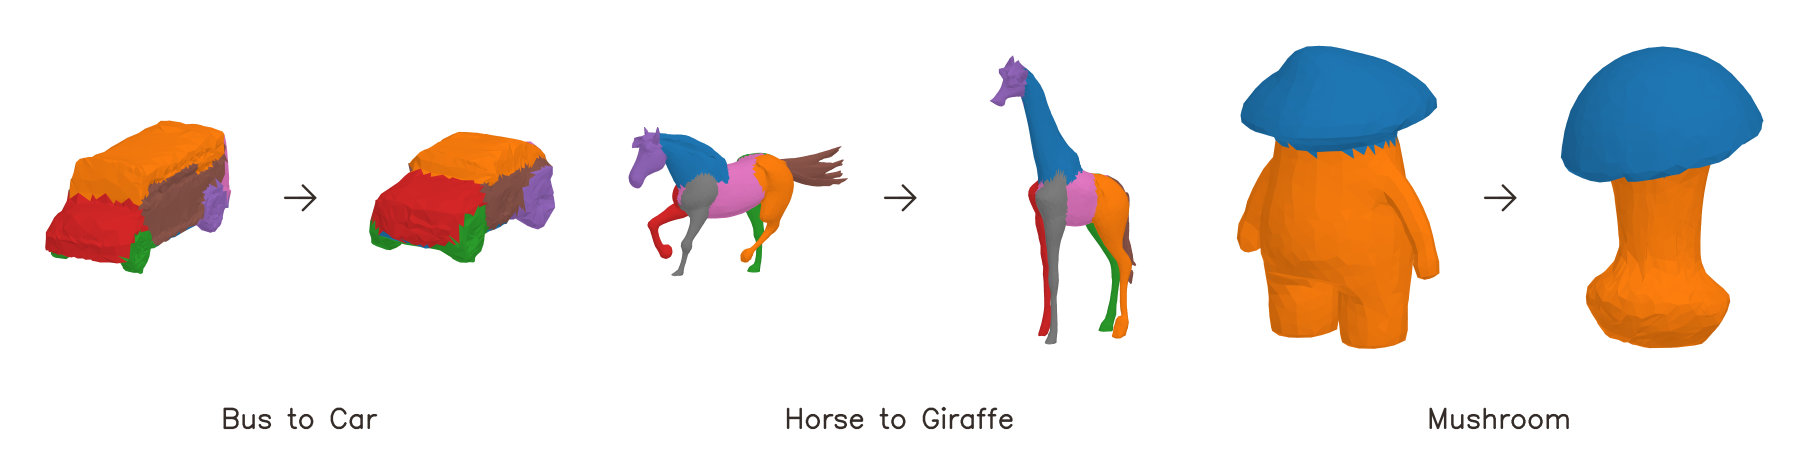
\includegraphics[width=0.92\textwidth]{figures/title_row_3pairs.png}

\vspace{1.2em}

{\large\bfseries Abstract\par}

\vspace{0.7em}

\end{center}

\begin{center}
\begin{minipage}{0.88\textwidth}
\small
\noindent
This project studies mesh-to-mesh deformation: given a source 3D shape, deform it so that it
matches a target shape while preserving the identity of meaningful parts. A purely global surface
loss, such as Chamfer distance, can make two shapes overlap geometrically while still mixing
parts: a leg can move toward a trunk, or a head can collapse into the body, if that reduces the
average point distance. This project's central idea is to add local, part-aware supervision from
PartField segmentations. Source and target meshes are segmented into unsupervised semantic
buckets; deformation is then optimized with a global Chamfer term, a per-bucket local Chamfer
term, and regularizers that discourage folding and excessive local distortion. The project began
as an extension of MeshUp, a score-distillation mesh deformation method driven by a $4.3$B-parameter
diffusion model, before being redirected into direct mesh-to-mesh deformation in 3D; that redirection 
is documented and explained in Appendix~\ref{app:meshup}.

The pipeline is evaluated on DenseCorr3D and on a self-created collection of SAM3D-reconstructed
meshes. The headline result is a graph-geodesic, same-pairs comparison against DenseMatcher's own
predicted correspondences: across all 23 available categories, with zero PartField-level
selection, this pipeline reaches mean \AUC{} $0.824$ against DenseMatcher's $0.672$, winning 21 of
23. A stricter no-preparation subset gives the same positive signal: among
12 categories without assisted orientation/preparation, the same range-averaged protocol still beats
DenseMatcher in 10 categories. This comparison, its methodology, and its scope are the central subject of
Section~\ref{sec:densematcher-fair}. Surface-quality evaluation on self-created SAM3D mesh pairs is
reported in Section~\ref{sec:surface-quality}. The report also documents concrete failure modes --
orientation mistakes, unstable part buckets, topology mismatch, and metric sensitivity to thin
evaluation regions -- with a full root-cause trace for the hardest produce categories.
\end{minipage}
\end{center}

\newpage
\tableofcontents
\newpage

\section{Introduction}

This report describes a project on 3D mesh deformation. In ordinary images, the data lives on a
flat grid of pixels. In 3D, the object has geometry: points have coordinates $(x,y,z)$, surfaces
have normals and curvature, and distances can be measured either through space or along the
surface itself. A useful deformation method should do more than move points until two shapes look
similar. It should keep the structure of the object coherent.

The motivating example is animal deformation. Suppose the source is a horse mesh and the target is
a giraffe mesh. A good result should stretch the neck, elongate the legs, and adjust the body without
losing the idea that legs match legs, head matches head, and body matches body. If we only
minimize global Chamfer distance, the optimizer sees an unordered set of surface samples. It can
reduce the average distance between the two surfaces while still matching the wrong parts. This is
the central ambiguity the project tries to reduce.

The pipeline developed here adds part-level structure by using PartField. PartField produces
unsupervised segmentation buckets for a mesh: not class labels such as ``leg'' or ``head'', but
consistent local regions that in most cases behave like semantic parts. These buckets are used as local
correspondence constraints. The deformation is still supervised by the target geometry, but it is
now asked to match source bucket $k$ to target bucket $k$ instead of treating all surface points as
interchangeable.

This project did not start from the pipeline described here; an earlier, image-semantic approach
built on MeshUp was tried first and deliberately redirected once its limits became clear. That
earlier direction, with full numbers, is documented in Appendix~\ref{app:meshup}.

\section{Motivation and Problem Setting}

\subsection{Why this problem matters}

3D shape deformation is useful whenever a known object must be adapted to a new shape while
remaining editable and interpretable. In animation, a character mesh may need to follow a new pose.
In graphics, a template mesh may need to fit a scanned object. In reconstruction, a generated mesh
may be close to the target object but still need geometric refinement. In all of these cases, the
mesh is not just a surface to be made close to another surface. It is also a structured object
whose parts should remain meaningful.

The motivating difficulty is that geometry and semantics are not the same thing. A global surface
distance can say that two shapes are close even when the correspondence is wrong. For example, if a
source animal has four legs and a target animal also has four legs, a global loss does not know
which leg should match which leg. If a target has a long neck or trunk, a global loss may pull a
nearby source region into that space even if the source region semantically belongs to the body.
The shape may look acceptable from one view while the underlying correspondence is poor.

This is especially important for meshes. A mesh carries topology, adjacency, and vertex identity.
If the deformation is later used for texture transfer, animation, interpolation, or correspondence
analysis, it matters whether the right vertices went to the right target regions. A pure
surface-fit objective cannot guarantee this.

\subsection{Why PartField is a useful prior}

The ideal supervision would be dense correspondence: for every point on the source surface, the
method would know the matching point on the target surface. This is rarely available outside
benchmarks. Manual part labels are easier than dense correspondences, but still expensive and not
available for arbitrary generated or reconstructed meshes. PartField~\cite{partfield} sits between
these two extremes. It gives a mesh decomposition into repeated local regions without manual
labels. The buckets are not perfect semantic labels, but they often align with object parts well
enough to guide optimization.

The important practical advantage is that PartField can be used on the same kinds of meshes that
the deformation pipeline already consumes. This means the project can use a single principle
across benchmark animals, SAM3D animals, vehicles, tools, and produce categories: deform globally,
but ask local regions to match local regions. The method is therefore not tied to one
category-specific skeleton or a hand-written list of parts. Figure~\ref{fig:horse-giraffe-buckets}
shows what this decomposition looks like in practice on a compatible pair.

\begin{figure}[H]
\centering
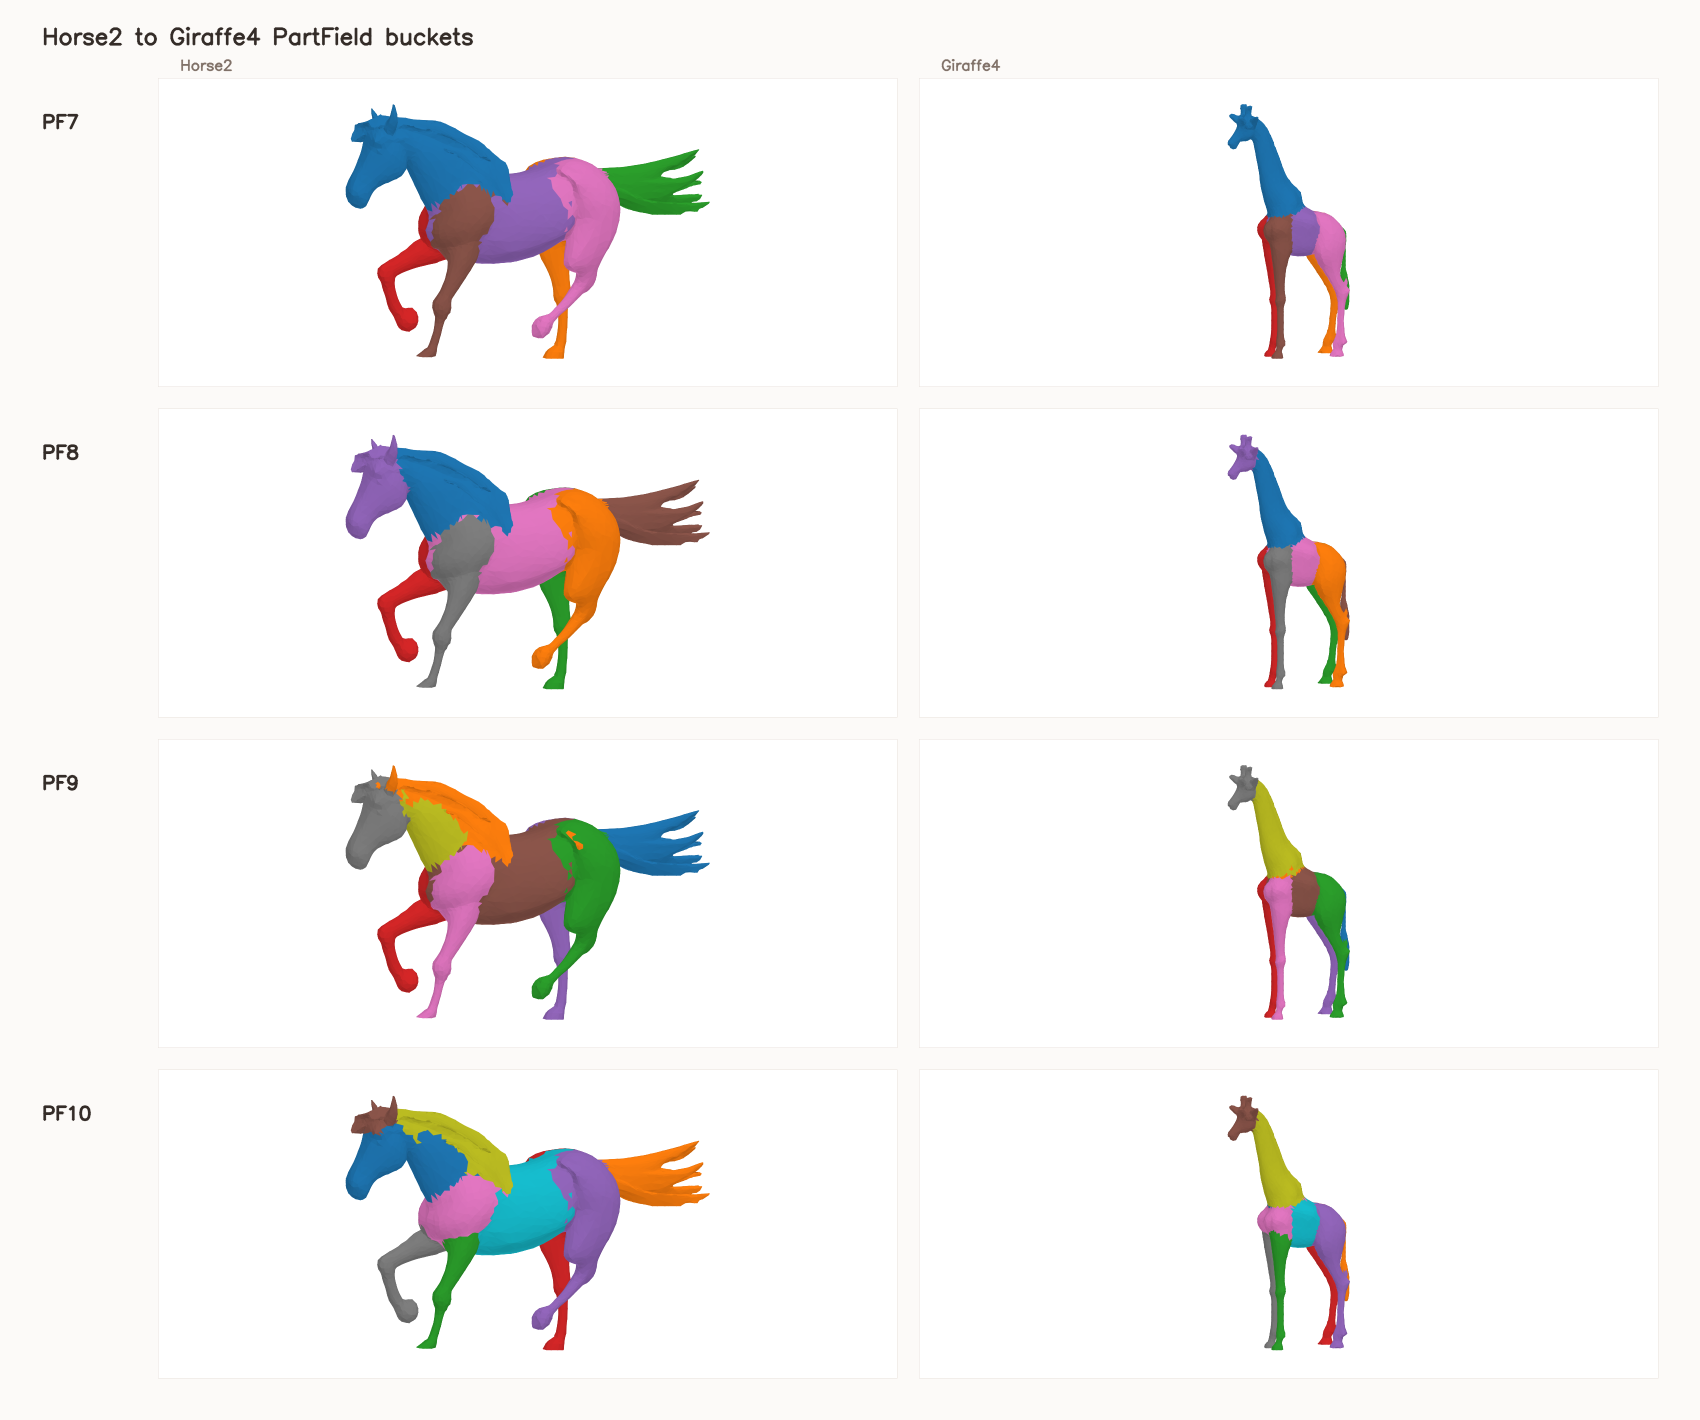
\includegraphics[width=0.82\textwidth]{figures/partfield_buckets_horse2_giraffe4.png}
\caption{PartField decomposition for Horse2 $\rightarrow$ Giraffe4, PF7--PF10.}
\label{fig:horse-giraffe-buckets}
\end{figure}

\subsection{Research questions}

The experiments are organized around four research questions:

\begin{enumerate}
  \item Does local PartField Chamfer improve semantic alignment compared with judging the result
  only by global surface proximity, \emph{and does it hold up against a real correspondence method
  scored on the exact same pairs}?
  \item Which PartField granularity is most useful, and is any single granularity stable enough
  across categories to be trusted as a fixed hyperparameter, rather than needing to be re-tuned
  per category?
  \item Do the deformed meshes remain geometrically clean when the local semantic loss is added,
  and does that hold across very different object domains?
  \item What kinds of shapes cause the pipeline to fail, and are those failures explainable?
\end{enumerate}

These questions also define the scope of the report. The project is a deformation pipeline evaluated with
correspondence metrics. The wording is important because DenseMatcher predicts correspondence
directly, whereas this project optimizes a source mesh until it becomes close to a target mesh.
DenseCorr3D annotations are used as an independent evaluator of the final deformation, and
Section~\ref{sec:densematcher-fair} is explicit about what a comparison against a direct
correspondence method can and cannot claim.

\subsection{What counts as success}

A successful deformation should satisfy three conditions. First, the output surface should be
close to the target. This is measured by Chamfer, \Fscore{}, and robust percentile distances.
Second, the output should preserve local semantic identity. On DenseCorr3D this is measured by
geodesic error, AUC, and same-bucket agreement. Third, the result should remain a plausible mesh.
This is addressed by regularization and inspected through qualitative figures and video showcases.

No single metric captures all three conditions. A result can have low Chamfer but poor semantic
alignment; it can have high AUC but a few severe tail failures; or it can match parts well but look
visually stretched. For that reason multiple metrics are taken into account. 

\subsection{Project goals}

Given this setting, the project has three concrete goals:

\begin{enumerate}
  \item Build a practical target-guided mesh deformation pipeline using global geometry, local
  part guidance, and regularization.
  \item Evaluate whether the deformed meshes are geometrically close to their targets.
  \item Evaluate whether the deformation preserves semantic correspondence, especially on
  DenseCorr3D where independent semantic-group annotations are available for evaluation, and
  directly against DenseMatcher's own predictions on the same pairs.
\end{enumerate}

\section{Basic Concepts}

\subsection{3D shapes, point clouds, and meshes}

A 3D shape is a geometric object embedded in three-dimensional space. In computation, the same
shape can be represented in several ways. A \emph{point cloud} is a set of points sampled from the
surface. It is simple and flexible, but it does not explicitly say which points are connected to
which other points. A \emph{mesh} adds this missing structure. In this project the mesh is a
triangular mesh, written as
\[
M = (V,F),
\]
where $V \in \mathbb{R}^{n \times 3}$ is the set of vertex coordinates and $F$ is a list of
triangular faces, each face indexing three vertices. The faces define the surface. Because
connectivity is known, a mesh supports surface normals, edge lengths, local neighborhoods,
geodesic distances, and deformation regularizers.

This distinction matters. Chamfer distance can be computed on point samples, but deformation is
applied to a mesh. If a method moves vertices without respecting mesh structure, the surface can
fold, stretch, tear visually, or develop distorted triangles. The pipeline therefore optimizes
surface matching and also regularizes the deformation field.

\subsection{Chamfer distance}
\label{sec:chamfer}

Chamfer distance is a standard way to compare two point sets. Let $P$ be points sampled from the
deformed source mesh and $Q$ be points sampled from the target mesh. The symmetric L1 Chamfer
distance used for evaluation in this project is
\[
d_{\mathrm{Chamfer}}(P,Q) =
\frac{1}{|P|}\sum_{p \in P}\min_{q \in Q}\|p-q\|_2
+
\frac{1}{|Q|}\sum_{q \in Q}\min_{p \in P}\|q-p\|_2 .
\]
% [ARTUR-FIX 8/9, revised per Artur comment 2026-10-06] L1 distance now defined via cite{chamferl1} instead of explained in prose.
Following~\cite{chamferl1}, the point-to-point term is L1-distance when $d(x,y) = \|x-y\|$ (the
unsquared Euclidean norm used above), and L2-distance when $d(x,y) = \|x-y\|^2$ -- the squared
variant used instead in this project's training loss (Section~\ref{sec:loss-function}). The first term asks whether every deformed source point is near the target. The second term asks
whether every target point is covered by the deformed source. The symmetry is important: otherwise
a small collapsed source could be close to part of the target while ignoring the rest.

Chamfer is powerful because it does not require point-to-point annotations. It is also limited
because it is blind to semantic identity. It only asks whether surfaces are close in space. This
project therefore implements local Chamfer terms computed separately inside PartField buckets
combined with global Chamfer.

\subsection{Why global Chamfer can be ambiguous}

Chamfer distance is often used because it is simple, differentiable almost everywhere, and does not
require the source and target meshes to have the same number of vertices. However, it treats both
surfaces as unordered samples. If two regions are spatially near, Chamfer has no reason to prefer
the semantically correct one. This creates three common ambiguities.

\begin{enumerate}
  \item Part swapping: If two legs are close, the optimizer may exchange them. For a
  visual rendering this may be difficult to notice, but for correspondence it is a real error.
  \item Part stealing: A large source region, usually the body, can cover target regions
  that should belong to a smaller part, such as a neck, ear, or tail.
  \item Collapse: A source surface can shrink toward a high-density target region and
  still reduce one side of the nearest-neighbor loss.
\end{enumerate}

The symmetric Chamfer formula reduces collapse because it also asks the source to cover the target,
but it still does not know which region should cover which target part. Local PartField Chamfer is
introduced exactly to reduce this freedom.

\subsection{Surface distance versus surface correspondence}

Surface distance and correspondence measure related but different properties. Surface distance asks
whether the deformed shape occupies the same space as the target. Correspondence asks whether a
source point moved to the correct target point or target region. This distinction is central to
interpreting the experiments. A deformation can have excellent surface distance if the final mesh
looks like the target, even when the mapping from source body parts to target body parts is
partially wrong. In contrast, a deformation can preserve correspondence well while still having high
surface distance if the source topology cannot represent the target geometry.

DenseCorr3D is useful because it supplies an independent semantic evaluator. The PartField losses
are unsupervised and local; DenseCorr3D annotations are held out and later used to ask whether those
unsupervised parts also agree with benchmark semantic regions. This separation is one of the
strongest aspects of the evaluation design, and it is exactly what makes the comparison in
Section~\ref{sec:densematcher-fair}.

\section{Background and Related Work}

\subsection{Template fitting and mesh deformation}

Classical mesh deformation often begins with a template mesh and tries to fit it to an observed
target. The target may be a scan, a point cloud, a depth reconstruction, or another mesh. Because
the template connectivity is preserved, the output remains easy to edit and compare. The difficulty
is that the optimization must balance flexibility with regularity. A very flexible deformation can
match the target surface but destroy the mesh. A very rigid deformation preserves the mesh but
cannot adapt to new shape proportions.

This project follows the template-fitting spirit: the source mesh acts as the template, and the
target mesh provides the geometric destination. The regularization terms keep the deformation from
becoming arbitrary, while the PartField terms give it semantic structure. The method therefore
lies between pure geometric registration and supervised correspondence learning.

\subsection{Dense correspondence and DenseMatcher}

Dense 3D correspondence methods aim to predict a mapping between surfaces. DenseCorr3D is a
benchmark of meshes with annotated semantic groups, released alongside
DenseMatcher~\cite{densematcher}, a learned method that predicts point-to-point correspondence
directly from category-level features -- it does not deform a mesh at all. Its goal is therefore
not identical to the goal of this project. Still, the DenseCorr3D metrics are valuable because they
answer an important question about the deformation: after the source has moved, did its semantic
regions land on the correct target regions? DenseMatcher's own predicted
correspondences were made available and can be scored on identical pairs with the identical
evaluator used for this project's own numbers -- turning ``compared against a published number''
into ``compared against the method itself.'' Section~\ref{sec:densematcher-fair} is dedicated to
that comparison and its caveats.

\subsection{Unsupervised part discovery}

Part discovery is the task of decomposing a shape into meaningful regions. In a supervised setting,
a dataset might label vertices as head, body, leg, handle, blade, seat, back, and so on. In this
project, that kind of supervision is not assumed. PartField provides a practical alternative by
producing feature fields that can be clustered into buckets. These buckets are not named semantic
classes, but they often align with repeated object structure.

The main risk is that unsupervised buckets can be inconsistent. If source bucket 3 is a leg but
target bucket 3 is partly body, the local loss becomes misleading. This is why the project tests
multiple granularities and why alignment is so important. PartField is not treated as an oracle; it
is treated as a useful but imperfect prior.

\subsection{Differentiable geometry losses}

Modern mesh optimization often uses differentiable geometric losses. Chamfer distance, normal-
consistency losses, edge-length penalties, and Jacobian-style regularizers~\cite{arap,njf} can all
be optimized with gradient-based methods. The project uses this family of ideas, but the key
addition is the local semantic decomposition. Instead of applying one global nearest-neighbor loss
to all samples, the optimizer also receives local nearest-neighbor losses inside corresponding
buckets. This small change has a large effect on the behavior of the optimization.

\section{Pipeline Overview}

The pipeline takes a source mesh and a target mesh as input. The source is the object that will be
deformed. The target is the object whose shape should be matched. The method keeps the source
topology: vertices move, but the original face connectivity remains. This makes the result easy to
compare with the original source, but it also means the method cannot create a new limb or a new
disconnected component from nothing.

\subsection{System overview: bucket selection, segmentation, deformation}
\label{sec:system-overview}

At the highest level the system has three stages (Figure~\ref{fig:pipeline-overview}): a
\emph{bucket selector} decides how many PartField buckets $K$ to use for a given source/target
pair; \emph{PartField} co-segments both meshes into $K$ buckets; and the \emph{deformation} stage
optimizes the source toward the target under Chamfer-style guidance plus regularization. The
implemented objective supports both whole-surface and per-bucket terms.

\begin{figure}[H]
\centering
\resizebox{\textwidth}{!}{% Bird's-eye system overview: LLM bucket selection -> PartField -> guided deformation.
% Companion to pipeline_tikz.tex, which expands the PartField + deformation stages
% (semantic extraction chain, loss terms, curriculum, evaluation branch) in full detail.
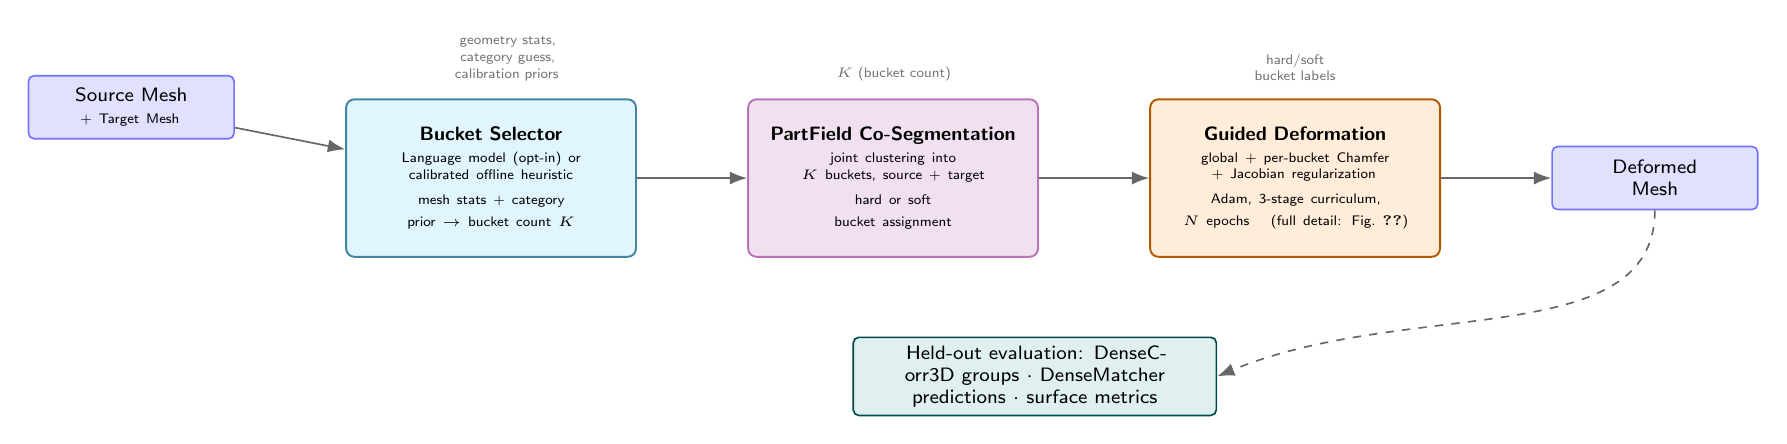
\begin{tikzpicture}[
  font=\sffamily\scriptsize,
  node distance=9mm and 14mm,
  stage/.style={draw, rounded corners=3pt, align=center, minimum height=20mm, inner sep=4pt, line width=0.7pt, text width=34mm},
  input/.style={draw, rounded corners=2pt, align=center, minimum height=8mm, inner sep=3pt, line width=0.6pt, text width=24mm, fill=blue!12, draw=blue!55},
  llm/.style={stage, fill=cyan!12, draw=cyan!60!black},
  sem/.style={stage, fill=violet!12, draw=violet!55},
  deform/.style={stage, fill=orange!15, draw=orange!70!black},
  ev/.style={draw, rounded corners=2pt, align=center, minimum height=8mm, inner sep=3pt, line width=0.6pt, text width=44mm, fill=teal!12, draw=teal!60!black},
  arr/.style={-{Latex[length=2.2mm]}, line width=0.6pt, draw=black!60},
  darr/.style={arr, dashed},
  lbl/.style={font=\sffamily\tiny, align=center, text width=26mm, color=black!55}
]

% --- inputs ---
\node[input] (src) {Source Mesh\\ \tiny + Target Mesh};

% --- stage 1: LLM bucket selector ---
\node[llm, right=of src, yshift=-9mm] (llmbox) {
  \textbf{Bucket Selector}\\[2pt]
  \tiny Language model (opt-in) or\\
  \tiny calibrated offline heuristic\\[3pt]
  \tiny mesh stats + category\\
  \tiny prior $\rightarrow$ bucket count $K$
};
\node[lbl, above=1mm of llmbox, xshift=2mm] {geometry stats,\\ category guess,\\ calibration priors};

% --- stage 2: PartField ---
\node[sem, right=of llmbox] (pfbox) {
  \textbf{PartField Co-Segmentation}\\[2pt]
  \tiny joint clustering into\\
  \tiny $K$ buckets, source + target\\[3pt]
  \tiny hard or soft\\
  \tiny bucket assignment
};
\node[lbl, above=1mm of pfbox] {$K$ (bucket count)};

% --- stage 3: guided deformation ---
\node[deform, right=of pfbox] (defbox) {
  \textbf{Guided Deformation}\\[2pt]
  \tiny global + per-bucket Chamfer\\
  \tiny + Jacobian regularization\\[3pt]
  \tiny Adam, 3-stage curriculum,\\
  \tiny $N$ epochs \quad (full detail: Fig.~\ref{fig:pipeline})
};
\node[lbl, above=1mm of defbox] {hard/soft\\ bucket labels};

% --- output ---
\node[input, right=of defbox] (out) {Deformed\\ Mesh};

% --- evaluation, dashed / held out ---
\node[ev, below=10mm of pfbox, xshift=18mm] (eval) {Held-out evaluation: DenseCorr3D groups $\cdot$ DenseMatcher predictions $\cdot$ surface metrics};

% --- arrows ---
\draw[arr] (src) -- (llmbox);
\draw[arr] (llmbox) -- (pfbox);
\draw[arr] (pfbox) -- (defbox);
\draw[arr] (defbox) -- (out);
\draw[darr] (out.south) .. controls +(0,-18mm) and +(24mm,10mm) .. (eval.east);

\end{tikzpicture}
}
\caption{Bird's-eye system overview. A bucket selector, implemented either with an LLM prompt or
with the offline heuristic, turns mesh geometry plus project/user priors into a single PartField
bucket count $K$. PartField then co-segments the pair, and deformation consumes those buckets as
in Figure~\ref{fig:pipeline}.}
\label{fig:pipeline-overview}
\end{figure}

Earlier experiments in this report chose PartField granularity by hand or by sweeping a fixed range
per category (Section~\ref{sec:densematcher-fair}); the selector automates that choice for a
specific source/target pair using an LLM prompt. It parses both meshes directly (vertex and face
counts, bounding-box aspect ratio, connected-component count),
guesses an object category from the mesh paths, and can receive short user notes about what has
worked or failed in previous DenseCorr3D/DenseMatcher experiments. The LLM-backed selector is
therefore not a blind zero-shot selector: it combines mesh statistics, the user's qualitative prior
for the category, and general object knowledge (for example, one or two buckets for smooth
single-part produce; more buckets for articulated animals, chairs, cars, or tools). This component
was built mainly so that the pipeline has one automated, complete path from a raw source/target pair
to a bucket count, rather than requiring a hand-chosen $K$ for every new pair.

A concrete example is \texttt{horse2}$\to$\texttt{giraffe}. The selector recognized the pair as an
animal case from the mesh paths and general object knowledge, and returned $K=6$ with confidence
$0.78$; a PartField co-segmentation preflight then validated that bucket count before handing the
pair to the deformation stage.

\subsection{The deformation stage in detail}

Figure~\ref{fig:pipeline} expands the PartField and deformation stages of
Figure~\ref{fig:pipeline-overview} into the full mechanism: the semantic-extraction chain, the
three loss terms and their combination, the curriculum, and the evaluation branch.

\begin{figure}[H]
\centering
\resizebox{0.88\textwidth}{!}{% Pipeline figure, native TikZ (no external renderer needed).
% A separately editable, freely colorable version of the same diagram lives in
% figures/pipeline.drawio -- open it in diagrams.net / draw.io to restyle or extend it;
% this file is what actually gets compiled into the PDF report.
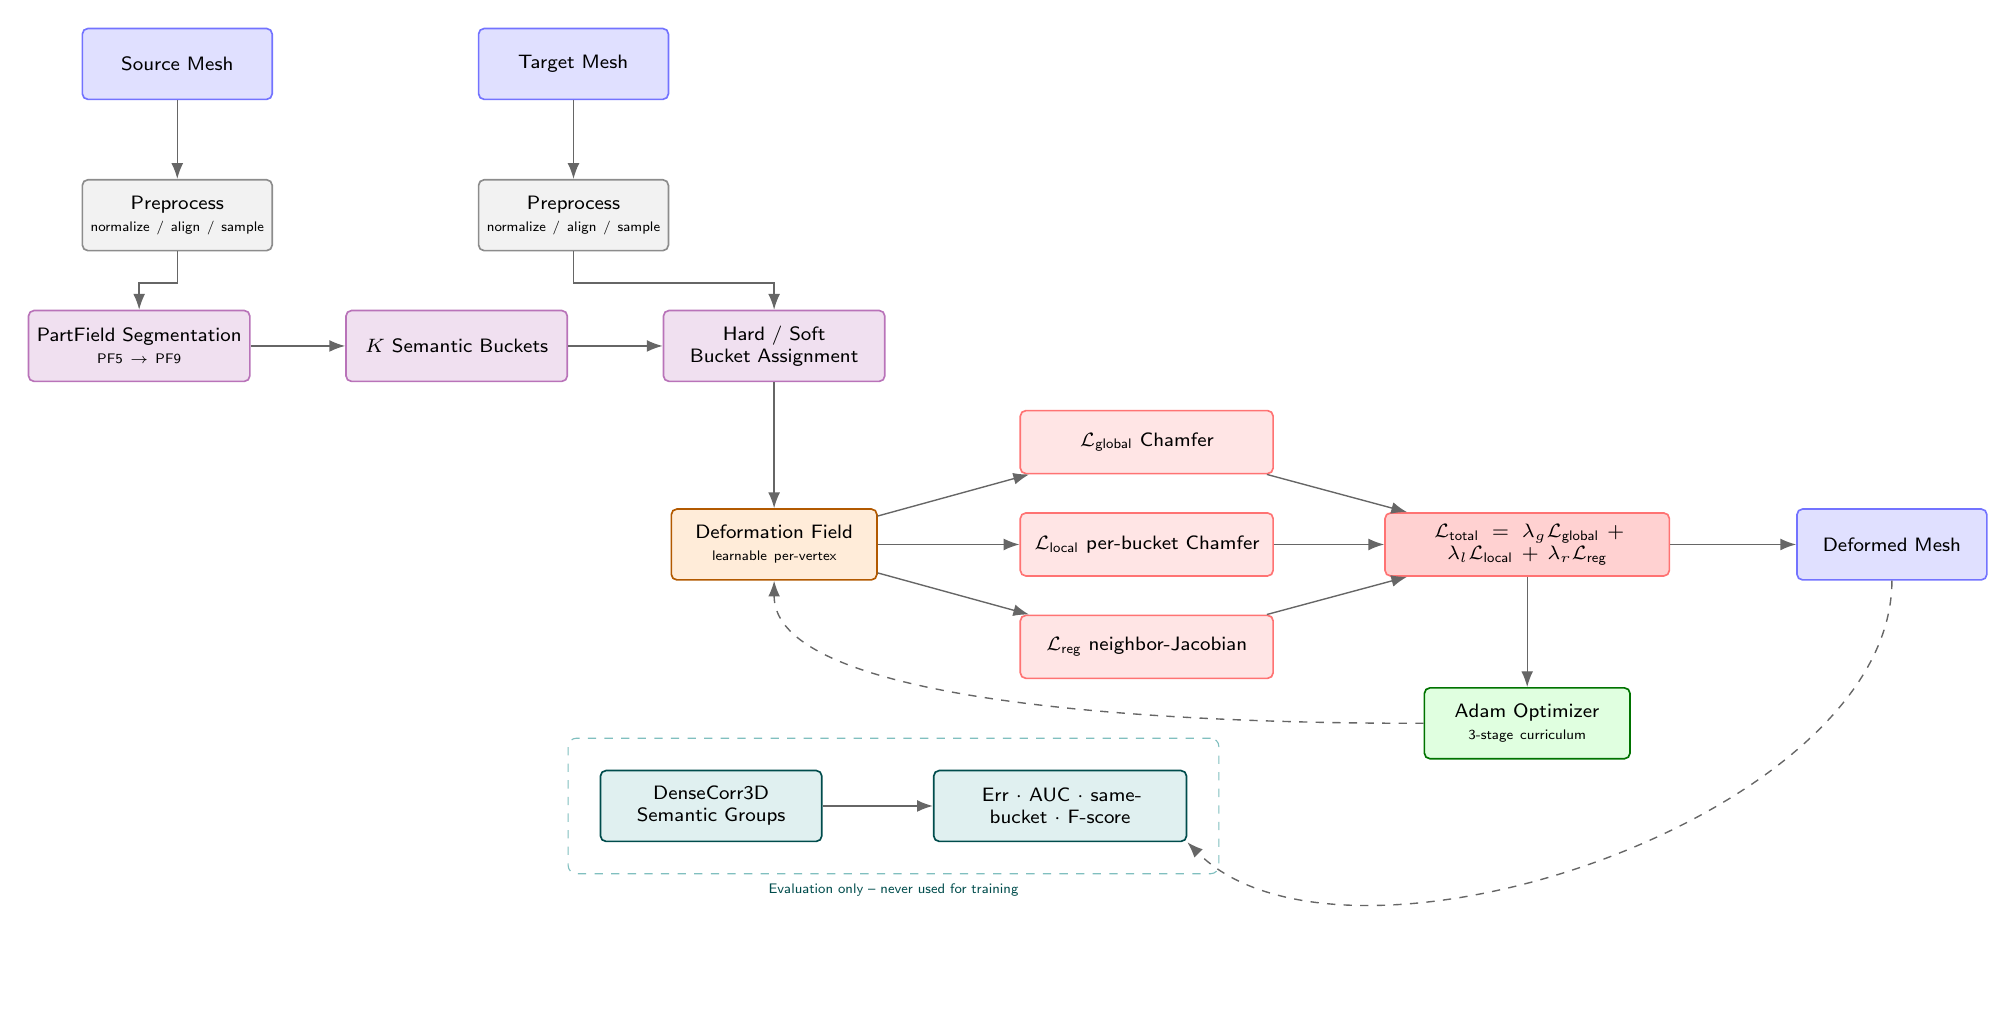
\begin{tikzpicture}[
  font=\sffamily\scriptsize,
  node distance=10mm and 12mm,
  box/.style={draw, rounded corners=2pt, align=center, minimum height=9mm, inner sep=3pt, line width=0.6pt, text width=26mm},
  input/.style={box, fill=blue!12, draw=blue!55, text width=22mm},
  prep/.style={box, fill=black!5, draw=black!45, text width=22mm},
  sem/.style={box, fill=violet!12, draw=violet!55, text width=26mm},
  deform/.style={box, fill=orange!15, draw=orange!70!black, text width=24mm},
  loss/.style={box, fill=red!10, draw=red!55, minimum height=8mm, text width=30mm},
  optim/.style={box, fill=green!12, draw=green!45!black, text width=24mm},
  ev/.style={box, fill=teal!12, draw=teal!60!black, text width=26mm},
  arr/.style={-{Latex[length=2mm]}, line width=0.5pt, draw=black!60},
  darr/.style={arr, dashed}
]

% --- row 1: inputs ---
\node[input] (src) {Source Mesh};
\node[input, right=26mm of src] (tgt) {Target Mesh};

% --- row 2: preprocessing ---
\node[prep, below=of src] (prepS) {Preprocess\\ \tiny normalize / align / sample};
\node[prep, below=of tgt] (prepT) {Preprocess\\ \tiny normalize / align / sample};

% --- row 3: semantic extraction ---
\node[sem, below=12mm of $(prepS)!0.5!(prepT)$, xshift=-30mm] (pf) {PartField Segmentation\\ \tiny PF5 $\to$ PF9};
\node[sem, right=of pf] (buckets) {$K$ Semantic Buckets};
\node[sem, right=of buckets] (assign) {Hard / Soft\\ Bucket Assignment};

% --- row 4: deformation + losses ---
\node[deform, below=16mm of assign] (deform) {Deformation Field\\ \tiny learnable per-vertex};

\node[loss, right=18mm of deform, yshift=13mm] (lglobal) {$\mathcal{L}_{\text{global}}$ Chamfer};
\node[loss, right=18mm of deform] (llocal) {$\mathcal{L}_{\text{local}}$ per-bucket Chamfer};
\node[loss, right=18mm of deform, yshift=-13mm] (lreg) {$\mathcal{L}_{\text{reg}}$ neighbor-Jacobian};

\node[loss, right=14mm of llocal, fill=red!18, text width=34mm] (ltotal) {$\mathcal{L}_{\text{total}} = \lambda_g\mathcal{L}_{\text{global}} + \lambda_l\mathcal{L}_{\text{local}} + \lambda_r\mathcal{L}_{\text{reg}}$};

\node[optim, below=14mm of ltotal] (opt) {Adam Optimizer\\ \tiny 3-stage curriculum};

\node[input, right=16mm of ltotal] (out) {Deformed Mesh};

% --- row 5: evaluation branch ---
\node[ev, below=24mm of deform, xshift=-8mm] (dc) {DenseCorr3D\\ Semantic Groups};
\node[ev, right=14mm of dc, text width=30mm] (metrics) {Err $\cdot$ AUC $\cdot$ same-bucket $\cdot$ F-score};

% --- arrows: preprocessing ---
\draw[arr] (src) -- (prepS);
\draw[arr] (tgt) -- (prepT);
\draw[arr] (prepS.south) -- ++(0,-4mm) -| (pf.north);
\draw[arr] (prepT.south) -- ++(0,-4mm) -| (assign.north);

% --- semantic extraction chain ---
\draw[arr] (pf) -- (buckets);
\draw[arr] (buckets) -- (assign);

% --- into deformation field ---
\draw[arr] (assign.south) -- ++(0,-4mm) -| (deform.north);

% --- losses ---
\draw[arr] (deform) -- (lglobal);
\draw[arr] (deform) -- (llocal);
\draw[arr] (deform) -- (lreg);
\draw[arr] (lglobal) -- (ltotal);
\draw[arr] (llocal) -- (ltotal);
\draw[arr] (lreg) -- (ltotal);
\draw[arr] (ltotal) -- (opt);
\draw[darr] (opt.west) .. controls +(-14mm,0) and +(0,-18mm) .. (deform.south);
\draw[arr] (ltotal) -- (out);

% --- evaluation branch (dashed, post-hoc only) ---
\draw[darr] (out.south) .. controls +(0,-30mm) and +(20mm,-20mm) .. (metrics.south east);
\draw[arr] (dc) -- (metrics);

% --- eval box outline ---
\begin{scope}[on background layer]
\node[draw=teal!50, dashed, rounded corners=3pt, fit=(dc)(metrics), inner sep=4mm,
      label={[font=\sffamily\tiny,teal!60!black]below:Evaluation only -- never used for training}] {};
\end{scope}

\end{tikzpicture}
}
\caption{Detailed PartField segmentation and guided-deformation stages.}
\label{fig:pipeline}
\end{figure}

Figure~\ref{fig:pipeline} shows the full process. At a high level:

\begin{enumerate}
  \item Normalize and orient the source and target meshes.
  \item Optionally, ask the bucket selector (Section~\ref{sec:system-overview}) to choose the
  PartField bucket count $K$ for this pair from mesh geometry and calibration
  priors; otherwise $K$ is set by hand.
  \item Extract PartField features and cluster them into $K$ part buckets.
  \item Build hard or soft bucket assignments for vertices and faces.
  \item Optimize a deformation field using the active Chamfer terms for that experiment family and
  regularization.
  \item Evaluate geometry on sampled surfaces and semantic alignment on held-out DenseCorr3D
  groups, and (Section~\ref{sec:densematcher-fair}) against DenseMatcher's own predictions, when
  available.
\end{enumerate}

The mesh
files provide vertices and faces; PartField inference produces features; clustering produces label
files; the deformation run produces a final mesh and intermediate visualizations; and the
evaluation scripts produce summaries. This makes the pipeline easy to debug because
each stage can be inspected separately. If a final deformation fails, one can ask: was the mesh
aligned correctly, did PartField produce reasonable buckets, did the optimizer move the right
regions, or did the metric penalize a thin semantic group?

\begin{table}[H]
\centering
\small
\begin{tabularx}{\textwidth}{lXX}
\toprule
Object & Meaning in the pipeline & Common failure if handled badly \\
\midrule
Source mesh & The topology that will be preserved and deformed. & Wrong source scale or pose creates unnecessary distortion. \\
Target mesh & The geometry the source should match. & Missing components or bad orientation mislead Chamfer and PartField. \\
PartField features & Per-point or per-region descriptors used for bucket construction. & Features can cluster by pose or noise rather than semantic part. \\
Bucket labels & Local regions used by the semantic Chamfer loss. & Bucket mismatch causes semantically wrong local pulls. \\
Final mesh & The source topology after deformation. & Can fit globally while still failing local correspondence. \\
\bottomrule
\end{tabularx}
\caption{The main intermediate objects in the pipeline and why each one matters.}
\label{tab:pipeline-objects}
\end{table}

\subsection{Source and target preparation}

All meshes are converted into the same coordinate convention before optimization. The pipeline
normalizes the source and target into a unit box, optionally rotates or aligns the mesh, and
samples points on the surface for loss evaluation. This step is simple but critical. If two animals
face opposite directions, or if a vegetable category has inconsistent stem orientation, PartField
buckets can be swapped even before deformation begins. Several failure cases in the project were
eventually traced to alignment rather than to the optimizer itself.

For DenseCorr3D experiments, the meshes come with semantic groups and correspondence annotations.
These annotations are not used in the deformation. They are held out for evaluation, where
they provide an independent way to ask whether a deformed source part lands on the correct target
part. For SAM3D experiments, the meshes are reconstructed from real photographs and are evaluated
mainly by surface geometry and PartField-region agreement, since no independent ground-truth
correspondence exists for self-created meshes.

\subsection{PartField buckets}

Figure~\ref{fig:giraffe-elephant-buckets} shows what PartField actually does to a pair of meshes
before the rest of this section works through the mechanics.

\begin{figure}[H]
\centering
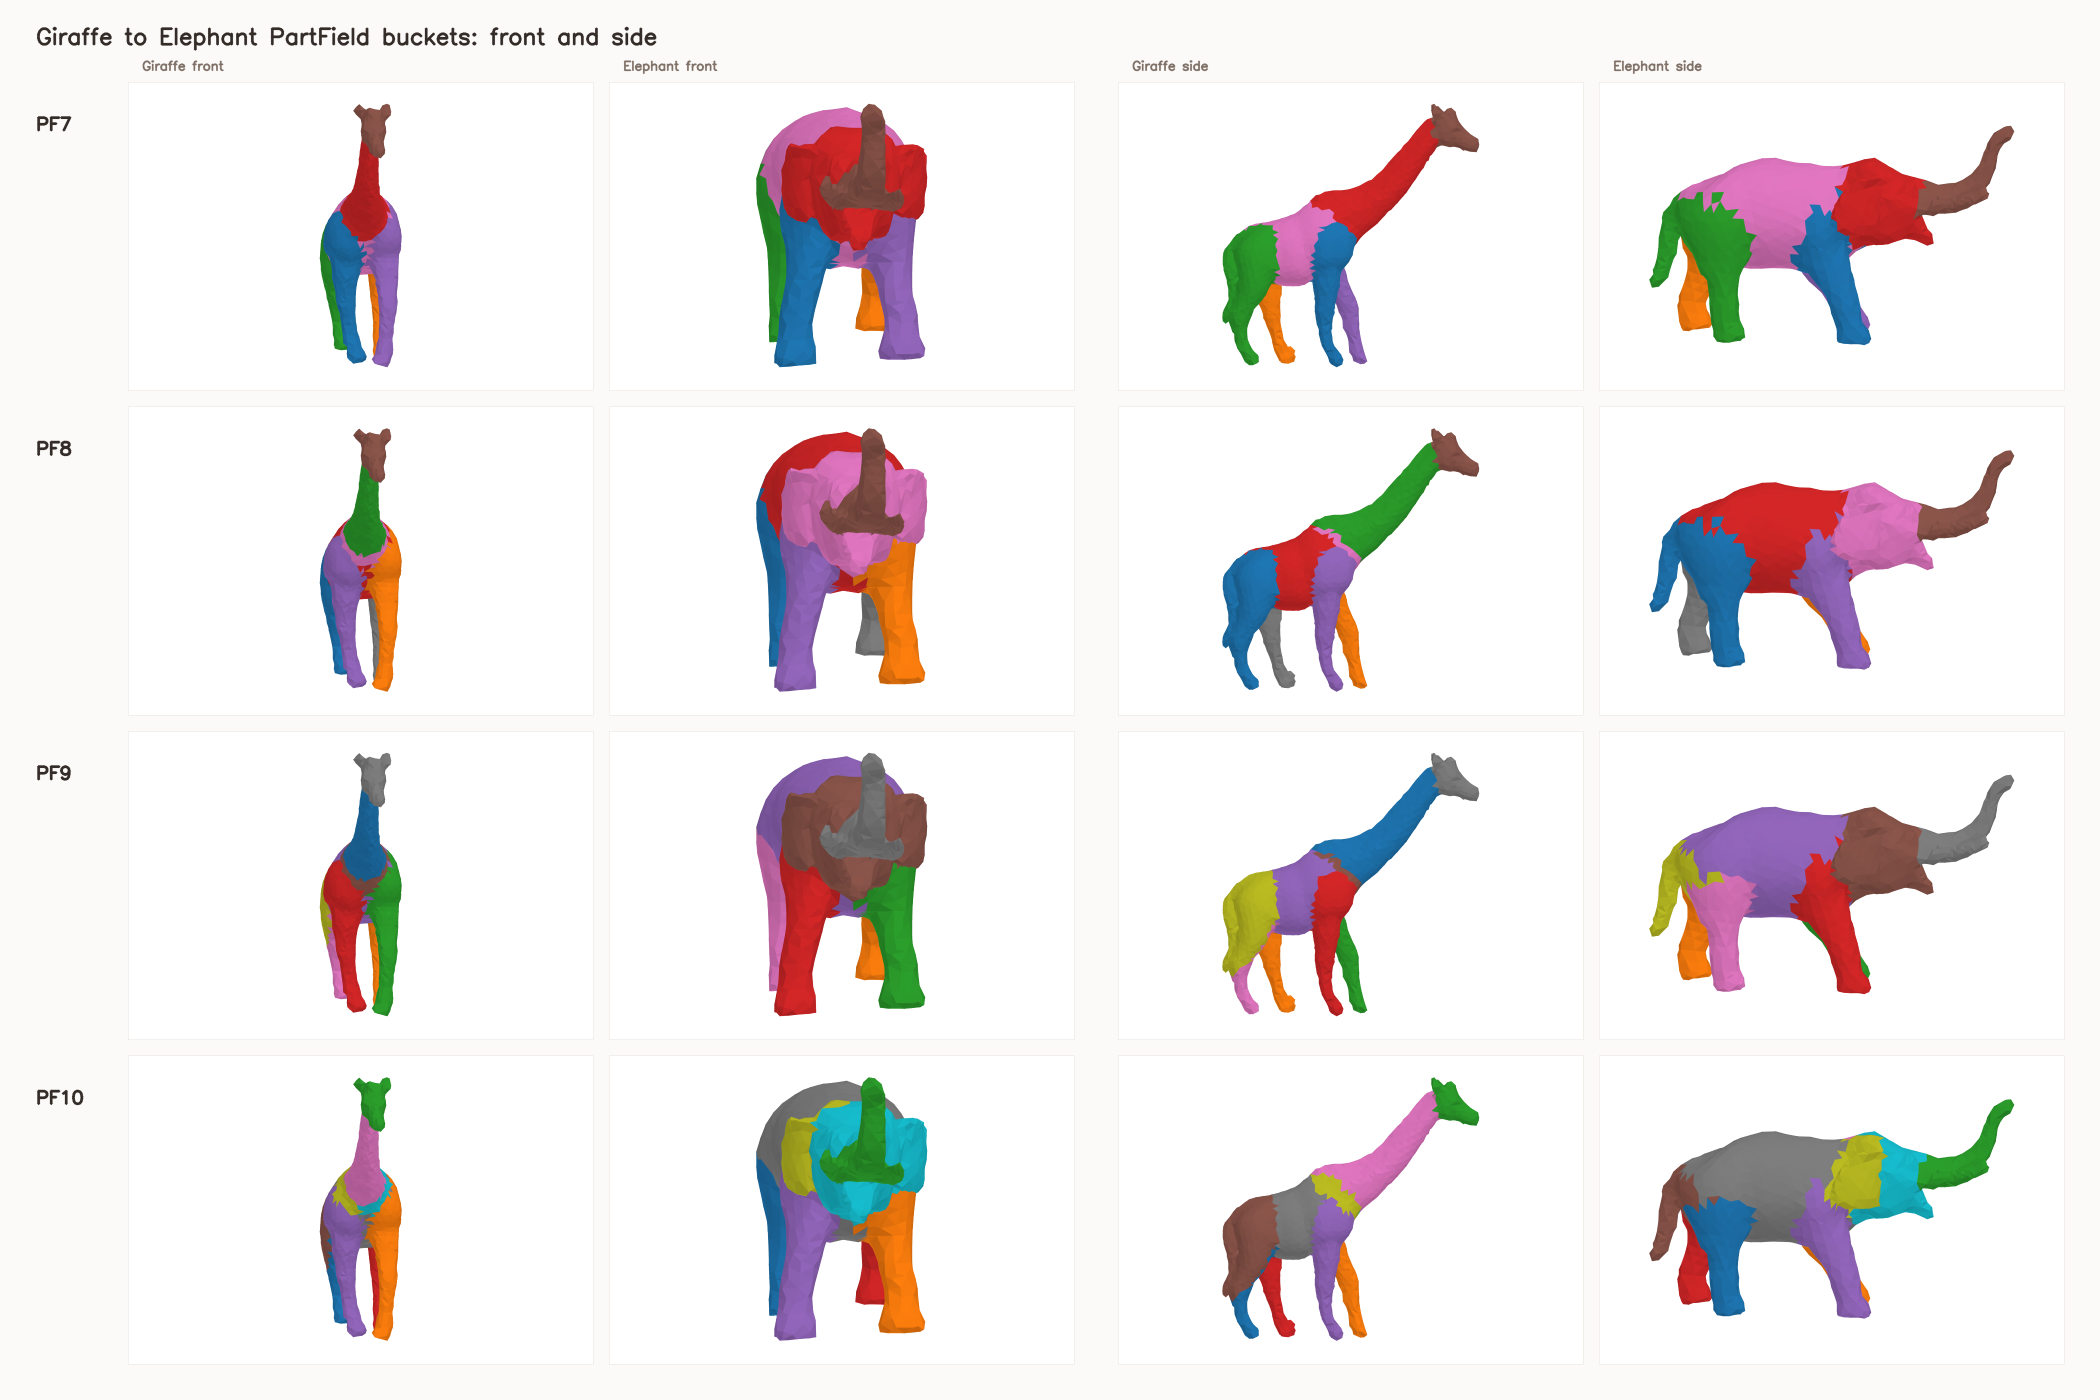
\includegraphics[width=0.88\textwidth]{figures/partfield_buckets_giraffe_elephant.png}
\caption{Giraffe-to-elephant PartField decomposition, PF7--PF10.}
\label{fig:giraffe-elephant-buckets}
\end{figure}

PartField~\cite{partfield} maps a mesh to local features that can be clustered into repeated
structural regions. The available granularities are written as PF1 through PF10 (a lower
number creates coarser buckets; a higher number creates finer buckets). Coarse buckets are more
stable but can merge distinct parts. Fine buckets can separate legs, head, body, ears, or tail more
clearly, but they can also become unstable when the source and target have different topology or
pose.

The important design choice is that the same bucket index is used on both source and target after
joint clustering or bucket balancing.
% [ARTUR-FIX 5/9] Added concrete description of how bucket matching (joint clustering) actually works.
Concretely, \emph{joint clustering} means the source and
target meshes' PartField feature vectors are pooled into one combined array before clustering, and
a single $K$-means model (with $K$ equal to the active bucket count) is fit on that pooled set;
splitting the resulting per-point cluster assignments back out by mesh is what gives source and
target their shared bucket indices, with no separate cross-mesh matching step required afterward --
bucket $k$ means the same region of PartField feature space on both meshes because both meshes'
points were clustered together in the first place. Bucket $k$ on the source is therefore encouraged to move near
bucket $k$ on the target. The buckets are not hand-labeled. The method never needs an explicit
label such as ``front left leg''. It only needs a consistent decomposition into local regions.

The project also distinguishes raw buckets from bucket-balanced buckets. Raw clustering can produce
a dominant bucket that covers most of the body and small buckets that contain only a few vertices.
This is a problem for local losses: a very large bucket can behave like another global Chamfer term,
while tiny buckets become noisy. Bucket balancing makes the local supervision more usable by
preventing one region from overwhelming the optimization, as shown concretely in
Figure~\ref{fig:bucket-balance-counts}.

\begin{figure}[H]
\centering
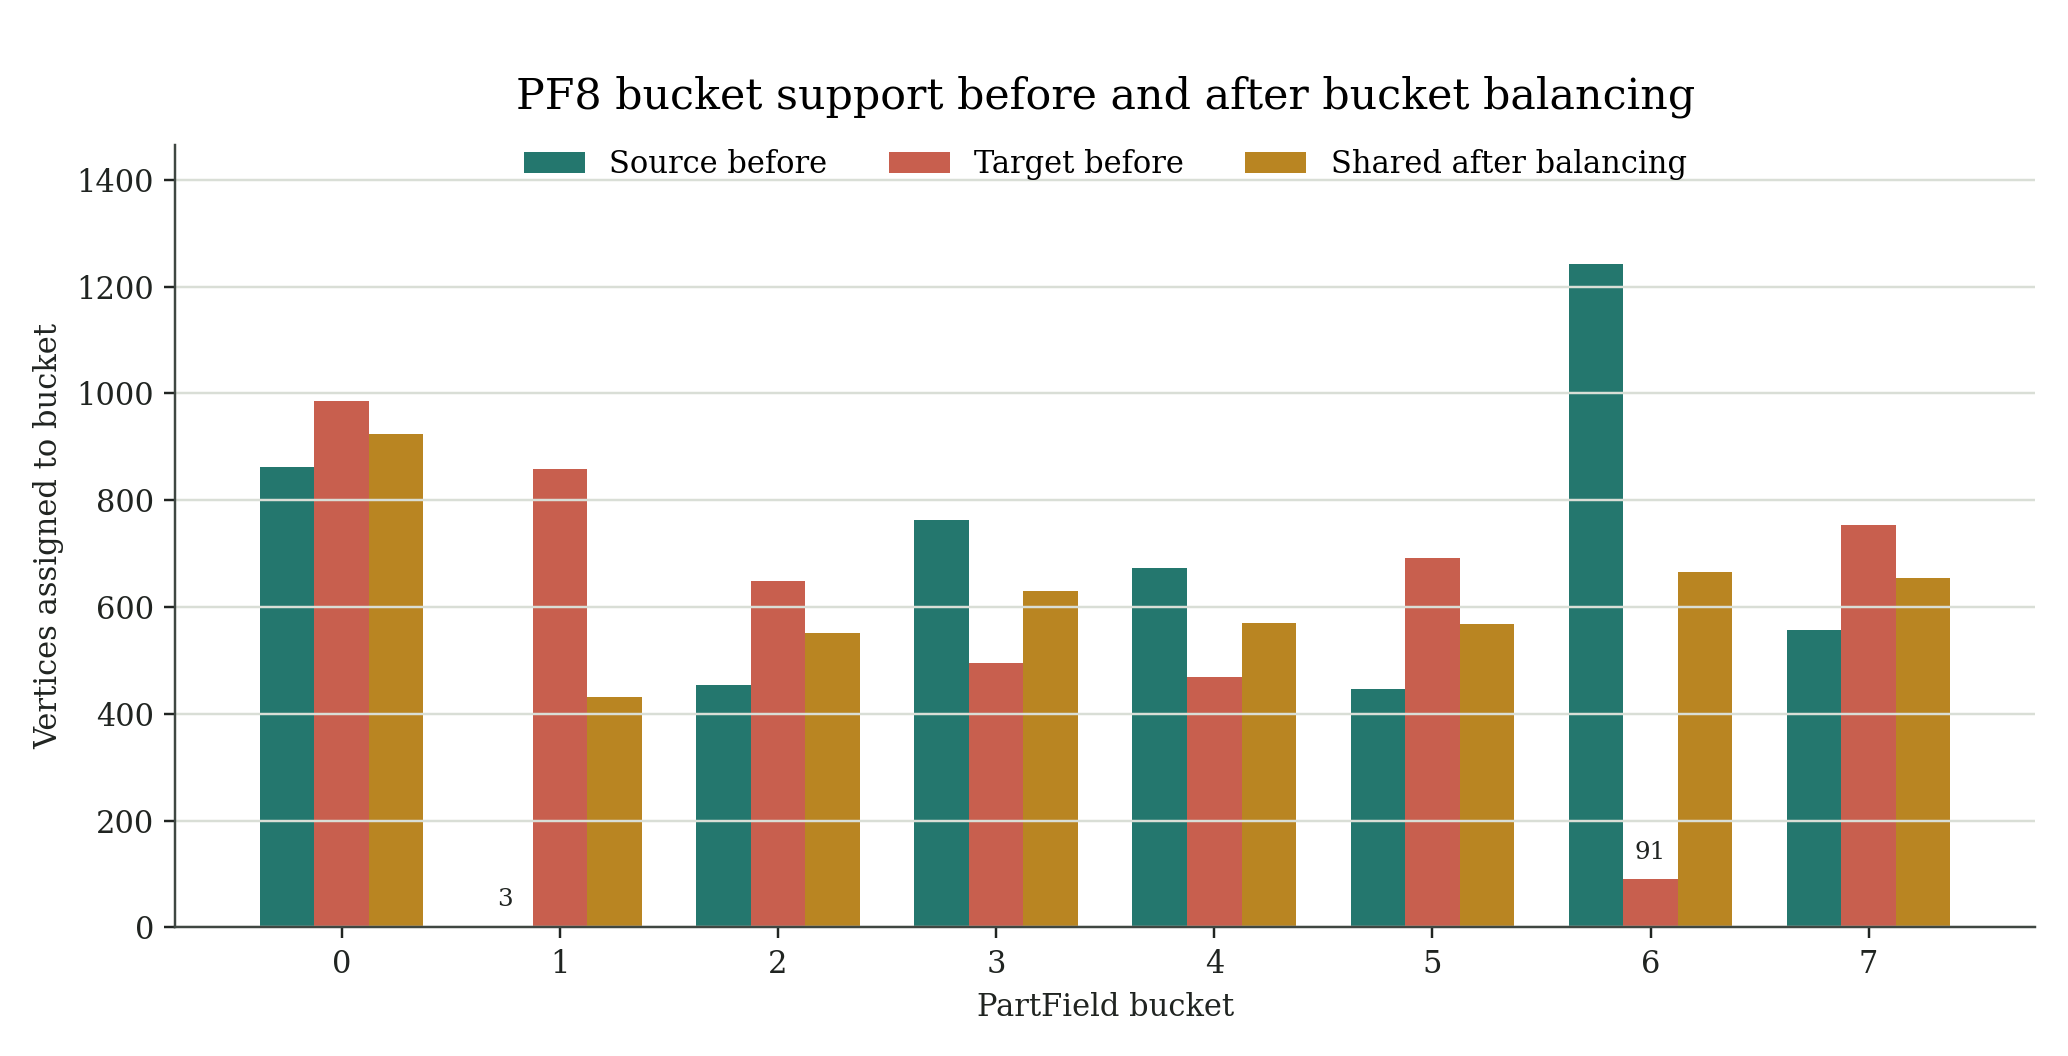
\includegraphics[width=0.78\textwidth]{figures/pf8_bucket_balance_counts.png}
\caption{PF8 bucket support before and after bucket balancing.}
\label{fig:bucket-balance-counts}
\end{figure}

\subsection{Deformation representation}
\label{sec:deformation-repr}

The deformation is parameterized as a learnable \emph{per-face Jacobian} field rather than raw
vertex positions: a $3\times3$ Jacobian is optimized for every face of the source mesh (via a
\texttt{NeuralJacobianFields.SourceMesh} object~\cite{njf}), and vertex positions are reconstructed
from the current Jacobians at every optimization step by a Poisson-style solve. This project
uses the Jacobian parameterization, optimized directly by Adam at learning rate $0.0025$. The
neighbor-Jacobian regularizer penalizes large differences between the Jacobians of adjacent faces,
which is what keeps the surface from folding or self-intersecting as it deforms; the reconstruction
step is what turns a smooth Jacobian field into a smooth vertex displacement.

Keeping the source topology has an important consequence: the result implicitly defines a
correspondence from the original source to the final deformed mesh. Vertex $i$ before optimization
is still vertex $i$ after optimization; only its position changes. This is useful for evaluation and
visualization because colors, labels, and source regions can be propagated directly (it is also
what makes the color-consistency fix behind Figure~\ref{fig:domain-animals} possible -- see its
caption). It is also why over-deformation is dangerous: if a group of source vertices is pulled
across the object to satisfy Chamfer, the mesh may still look near the target, but the inherited
source labels reveal that the semantic mapping is wrong.

\subsection{Loss function}
\label{sec:loss-function}

The optimization objective is
\[
\mathcal{L}_{\mathrm{total}} =
\lambda_g \mathcal{L}_{\mathrm{global}}
+
\mathcal{L}_{\mathrm{local}}
+
\mathcal{L}_{\mathrm{reg}} .
\]

The global term $\mathcal{L}_{\mathrm{global}}$ is the Chamfer distance~\cite{psgn} between samples
from the entire deformed source surface and samples from the target surface. The local term is a sum of \emph{asymmetric} Chamfer distances over active PartField buckets
(buckets with at least $12$ vertices on both sides by default):
\[
\mathcal{L}_{\mathrm{local}} =
\sum_{k \in \mathcal{K}_{\mathrm{active}}}
d^{\,\mathrm{asym}}_{\mathrm{Chamfer}}(P_k,Q_k),
\]
where $P_k$ are samples from the deformed source bucket $k$ and $Q_k$ are samples from the target
bucket $k$. Concretely, for $p \in P_k$ write $q^*(p) = \arg\min_{q \in Q_k}\lVert p-q\rVert_2$ for
its nearest target neighbor, and for $q \in Q_k$ write $p^*(q) = \arg\min_{p \in P_k}\lVert
q-p\rVert_2$ for its nearest source neighbor. Call $p$ \emph{claimed} if $p = p^*(q)$ for at least
one $q \in Q_k$ (some target point in the bucket needs exactly this source point), giving it weight
$w(p) = 1$; an unclaimed source point instead gets weight $w(p) = \gamma < 1$. Then
\[
d^{\,\mathrm{asym}}_{\mathrm{Chamfer}}(P_k,Q_k) =
\alpha \cdot \frac{\sum_{p \in P_k} w(p)\,\lVert p-q^*(p)\rVert_2^2}{\sum_{p \in P_k} w(p)}
\;+\;
\beta \cdot \frac{1}{|Q_k|}\sum_{q \in Q_k}\lVert q-p^*(q)\rVert_2^2 ,
\]
with source-to-target weight $\alpha \in [0.30,0.40]$ (best-performing presets use $\alpha=0.35$,
denoted \texttt{asym035} in job names) and target-to-source weight $\beta = 1.0$; the unmatched-point
down-weight $\gamma$ (tested at $\gamma=0.15$, the \texttt{mutual015} preset) is only active when
explicitly enabled. Unlike the global Chamfer distance in Section~\ref{sec:chamfer} (raw
$\lVert\cdot\rVert_2$, for interpretability in real units), the local term is computed on squared
distances, the standard choice for a smoother optimization signal; only the reporting metrics in
Section~\ref{sec:eval-metrics} use the raw distance.

Both mechanisms exist to counter the same failure mode. Under a plain, evenly-weighted per-point
Chamfer term, a source point that no target point in the bucket actually needs (i.e.\ unclaimed) is
still pulled at full strength toward its own single nearest target point; because nothing else
constrains that point to stay near its neighbors, the result can be a thin spike or an
over-elongated limb rather than a smooth deformation. Lowering $\alpha$ reduces how hard every
source point is pulled toward the target on its own, and down-weighting unclaimed points removes
most of the pull specifically for the points most likely to spike. Figure~\ref{fig:spike-failure} in
Appendix~\ref{app:spike-failure} shows exactly this failure on an early bulldog$\to$dachshund run
that used the chamfer-only objective before this weighting was introduced. This is the main semantic
guidance in the method. In the headline DenseMatcher comparison (Section~\ref{sec:densematcher-fair}),
the saved run configurations set $\lambda_g=0$ and use the PartField/local term as the active
geometric fitting signal; global-only and global+PartField variants are therefore not folded into
those headline numbers.

The regularization term discourages unrealistic deformations:
\[
\mathcal{L}_{\mathrm{reg}} = \lambda_{\mathrm{jn}}\mathcal{L}_{\mathrm{neighbor\text{-}Jacobian}}
+ \lambda_{\mathrm{jump}}\mathcal{L}_{\mathrm{edge\text{-}jump}}
+ \lambda_{\mathrm{es}}\mathcal{L}_{\mathrm{edge\text{-}stretch}}.
\]
The neighbor-Jacobian term penalizes differences between the Jacobians of adjacent faces, acting
directly on the deformation's own parameterization (Section~\ref{sec:deformation-repr}). The
edge-displacement-jump term penalizes cases where the displacement difference between two
edge-connected vertices exceeds a threshold fraction of the original edge length, with an extra
penalty on the single worst violation -- this is the term most directly responsible for preventing
self-crossing in thin, elongated parts such as necks and legs.

\begin{table}[H]
\centering
\small
\begin{tabularx}{\textwidth}{lXX}
\toprule
Loss component & What it measures & Why it is needed \\
\midrule
Global Chamfer & Distance between the whole deformed source surface and the whole target surface. & Gives the optimizer the overall target shape. \\
Local Chamfer & Asymmetric distance between matching PartField buckets. & Reduces part swapping and part stealing. \\
Bucket weights & Relative influence of each bucket. & Keeps small parts from disappearing under large body regions. \\
Neighbor-Jacobian & Agreement between nearby per-face Jacobians. & Prevents abrupt discontinuities and folding across adjacent faces. \\
Edge stretch / jump penalties & Changes in edge length or displacement across edges. & Discourages folds, spikes, and extreme local stretching. \\
\bottomrule
\end{tabularx}
\caption{Interpretation of the main loss components.}
\label{tab:loss-components}
\end{table}

\subsection{Evaluation metrics}
\label{sec:evaluation}
\label{sec:eval-metrics}

The report uses several metrics, defined here using the same $P$ (deformed
source samples) and $Q$ (target samples) notation as the Chamfer distance in
Section~\ref{sec:system-overview}.

\Fscore{} is the harmonic mean of precision and recall at a unit-box threshold $\tau = 0.02$:
\[
\mathrm{Prec}(\tau) = \frac{1}{|P|}\sum_{p \in P} \mathbb{1}\!\left[\min_{q \in Q}\|p-q\|_2 < \tau\right],
\qquad
\mathrm{Rec}(\tau) = \frac{1}{|Q|}\sum_{q \in Q} \mathbb{1}\!\left[\min_{p \in P}\|q-p\|_2 < \tau\right],
\]
\[
\mathrm{F@}\tau = \frac{2\,\mathrm{Prec}(\tau)\,\mathrm{Rec}(\tau)}{\mathrm{Prec}(\tau) + \mathrm{Rec}(\tau)}.
\]
Precision asks what fraction of deformed-source surface samples lie within $\tau$ of the target;
recall asks what fraction of target samples are covered by the deformed source. Higher is better.

The robust $p95$ distance is the $95$th percentile of the same per-point nearest-neighbor
distances used by Chamfer, $p95 = Q_{0.95}\big(\{\min_{q \in Q}\|p-q\|_2 : p \in P\}\big)$, where
$Q_{0.95}$ denotes the $95$th-percentile operator. It is useful because a method can have good mean
Chamfer while a small part of the mesh is very wrong. Lower $p95$ means fewer large local errors.

DenseCorr3D-style correspondence evaluation uses normalized geodesic error. DenseMatcher defines
the semantic-group version of this metric as the distance from the predicted target point to the
nearest point in the correct ground-truth semantic group~\cite{densematcher}. For a source point
$i$ with predicted target correspondence $\hat{y}_i$ and target semantic group $G_i^{*}$,
\[
e_i = \frac{\min_{y \in G_i^{*}} d_{\mathrm{geo}}(\hat{y}_i, y)}{\sqrt{\mathrm{area}(\text{target})}},
\]
where $d_{\mathrm{geo}}$ is graph-geodesic (shortest-path) distance on the target mesh and the
$\sqrt{\mathrm{area}}$ term normalizes for object scale.
% [ARTUR-FIX 3/9] Explicitly defines the pipeline's own (induced) correspondence, vs. DenseMatcher's direct prediction.
$\hat{y}_i$ means something different for
each method being scored this way. DenseMatcher predicts $\hat{y}_i$ directly: it is the point its
\texttt{surface\_map}/\texttt{surface\_map\_inv} output assigns to source point $i$. This pipeline
does not output a correspondence map at all (Section~\ref{sec:system-overview}), so $\hat{y}_i$ is
instead induced from its deformation output after the fact: source vertex $i$ keeps its identity
through optimization (Section~\ref{sec:deformation-repr}), so $\hat{y}_i$ is defined as the nearest
target-mesh vertex, by Euclidean distance in the same normalized coordinates used throughout this
section, to vertex $i$'s final deformed position. This is the same nearest-neighbor lookup already
used by every Chamfer-based term and metric in this report; evaluation simply reuses it to name a
correspondence rather than only a distance. The report follows the evaluator output
and reports
\[
\mathrm{Err} = 100 \cdot \frac{1}{n}\sum_i e_i ,
\]
so an Err value of $4.77$ means mean normalized semantic geodesic error $0.0477$. Let
$\Phi(t) = \frac{1}{n}\sum_i \mathbb{1}[e_i < t]$ be the fraction of points correct at threshold
$t$; AUC integrates this curve up to a normalized threshold of $0.25$ and rescales it to $[0,1]$:
\[
\mathrm{AUC} = \frac{1}{0.25}\int_0^{0.25} \Phi(t)\,dt .
\]
For AUC, higher is better; for Err, lower is better.

The remaining reported metrics are surface diagnostics. Symmetric \Chamfer{} is the mean
nearest-neighbor surface distance in both directions in unit-box coordinates. Normal consistency is
the mean absolute dot product between matched surface normals, so higher values indicate smoother
normal agreement. Semantic \Chamfer{} and semantic \Fscore{} repeat the surface metrics inside
matching semantic or PartField regions rather than over the whole object. Same-bucket agreement is
the fraction of evaluated points whose predicted target neighbor falls in the expected bucket or
semantic group; it is useful as a coarse label-consistency check but does not replace geodesic
AUC/Err.

\subsection{Runtime and computational cost}
\label{sec:runtime}

All deformation runs use a single GPU on a shared Slurm cluster. Table~\ref{tab:runtime} compares
the currently submitted resource request (\texttt{gpu:1}, $8$ CPUs, $10$\,GB RAM, $30$-minute
limit) against measured usage: peak RAM stays below $1.8$\,GiB and wall-clock time ranges from
about $4$ to $18$ minutes across job families -- a small fraction of the $80{,}000$+ diffusion
evaluations and $40$--$64$\,GB requests the earlier MeshUp/SDS branch needed
(Appendix~\ref{app:meshup}).

\begin{table}[H]
\centering
\small
\begin{tabular}{lccc}
\toprule
Resource & Currently submitted & Actual measured need & Recommended request \\
\midrule
GPU & 1 $\times$ H100 & 1 GPU (single-GPU pipeline) & 1 GPU \\
CPUs & 8 & $\sim$0.7--1.0 core average & 2 (4 to be safe) \\
RAM & 10\,GB & max 1.8\,GiB system RAM & 4\,GB (8\,GB to be safe) \\
Time limit & 30\,min & $\sim$4--18\,min & 20--30\,min (safe margin) \\
\bottomrule
\end{tabular}
\caption{Slurm resource request vs.\ measured usage, standard deformation jobs.}
\label{tab:runtime}
\end{table}

% [ARTUR-FIX 6/9, shortened per Artur comment 2026-10-06] Trimmed DenseMatcher stage breakdown; kept the headline ratio.
This cost should be weighed against DenseMatcher's own reported inference cost: DenseMatcher takes
$8.4$--$12.4$ seconds per pair on a single A100 GPU, a single feed-forward pass with no iterative
optimization~\cite{densematcher}. This pipeline's $4$--$18$ minutes per pair
(Table~\ref{tab:runtime}), measured on a comparable or faster GPU (H100 rather than A100), is
therefore roughly $20$ to $130\times$ slower, since it solves a per-pair iterative optimization
problem instead of one forward pass -- a real advantage for DenseMatcher that the accuracy
comparison in Section~\ref{sec:densematcher-fair} does not capture on its own.

\subsection{Reproducibility and held-out evaluation}

The implementation is organized around repeatable experiment families. Each run stores its
configuration, final mesh, visualizations, and evaluation outputs. This matters because mesh
deformation experiments are sensitive to preprocessing, PartField level, target choice, and loss
weights.

DenseCorr3D's semantic groups are used only to score a deformation after the fact. They are never
read by the deformation stage, the loss function, or the bucket selector: the only signal PartField
and the optimizer ever see is geometry. This separation is what makes the DenseCorr3D-based numbers
in this report an external check on the result.

\section{Data and Assets}
\label{sec:data-assets}

\subsection{DenseCorr3D}

DenseCorr3D is a dense 3D correspondence benchmark with meshes, semantic groups, and evaluation
tools for surface correspondence, released alongside DenseMatcher~\cite{densematcher}. In this
project, its $23$ categories -- animals, produce, tools, vehicles, and containers -- provide an
external test bed for semantic deformation: after deforming a source mesh into a target mesh, the
DenseCorr3D annotations measure whether corresponding surface regions land in the right place, and
the breadth of categories is what lets the report ask where PartField-guided deformation
generalizes and where it fails.

\subsection{SAM3D and project meshes}

The project also uses a self-created set of meshes reconstructed with SAM3D~\cite{sam3d} from
single real photographs (each paired with a SAM2-derived mask) and then processed into the same
mesh deformation pipeline. These assets are useful because they test the method on realistic
meshes outside the benchmark distribution: imperfect components, noisy reconstructions, pose
differences, and inconsistent scale that curated benchmark meshes do not have.

\begin{table}[H]
\centering
\small
\begin{tabularx}{\textwidth}{>{\raggedright\arraybackslash}p{0.22\textwidth}>{\raggedright\arraybackslash}p{0.18\textwidth}>{\raggedright\arraybackslash}p{0.28\textwidth}>{\raggedright\arraybackslash}X}
\toprule
Dataset / split & Scale & Role in the report & Main caveat \\
\midrule
DenseCorr3D categories & 23 categories; 2328 evaluated (directed pair, PF-setting) rows & Main semantic alignment benchmark against held-out DenseCorr3D groups and DenseMatcher's released predictions. & Graph-geodesic local evaluator; PF ranges are category-specific and range-averaged. \\
SAM3D-created animals & 14 meshes; 8 directed pairs evaluated & Self-created reconstructed animal set for surface-quality evaluation and video showcase. & No independent dense correspondence ground truth. \\
SAM3D-created vehicles & 25 meshes; 5 directed pairs evaluated & Rigid, sharp-edged non-animal test outside DenseCorr3D. & Markedly weaker than animals under the identical PartField-only recipe. \\
Cross-dataset chain examples & 2 directed pairs & Transfer between benchmark-like and reconstructed assets. & Small qualitative and diagnostic set. \\
\bottomrule
\end{tabularx}
\caption{Combined dataset inventory and evaluation role.}
\label{tab:datasets}
\end{table}

\section{Fair Comparison Against DenseMatcher Under Graph-Geodesic Evaluation}
\label{sec:densematcher-fair}

This is the central quantitative section of the report. DenseMatcher's own predicted
correspondences (\texttt{surface\_map} / \texttt{surface\_map\_inv}, DenseMatcher's method-0
forward functional-map output) were computed for the DenseCorr3D test split. Both
methods are scored with the identical graph-geodesic evaluator -- Dijkstra shortest paths on the
target mesh, since the official DenseCorr3D geodesic distance matrices are not available -- on the
identical directed pairs, and the result is reported with its evaluation caveats. Everywhere in
this section, ``beats DenseMatcher'' means beats DenseMatcher's released
predictions under this graph-geodesic evaluation protocol.

\subsection{Methodology}

Both methods are scored against the identical DenseCorr3D \texttt{groups.txt} semantic labels,
using the identical graph-geodesic (Dijkstra) distance, identical $\sqrt{\mathrm{area}}$
normalization, and identical $\mathrm{AUC}[0,0.25]$/Err formula, where Err is mean normalized
semantic geodesic error multiplied by $100$ (Section~\ref{sec:evaluation}).
DenseMatcher's number in every table below is restricted to the precise (source, target) directed
pairs this pipeline was evaluated on, and direction was
matched explicitly (\texttt{surface\_map} vs.\ \texttt{surface\_map\_inv}) per pair. DenseMatcher's predictions never touched the deformation pipeline: the only active Chamfer
term in every run reported here is the PartField/local term, used
together with the same regularizers described in Section~\ref{sec:deformation-repr} as in every
other experiment family. DenseMatcher's \texttt{.npz} files only enter the project in a separate
evaluation script, after every deformation run already existed.

% [ARTUR-FIX 1/9] New paragraph: DenseMatcher ran on the original, unreoriented meshes.
DenseMatcher's predictions were computed on DenseCorr3D's released meshes and were never
regenerated by this project: the \texttt{surface\_map}/\texttt{surface\_map\_inv} \texttt{.npz}
files were supplied precomputed (Section~\ref{sec:data-assets}) and read directly by the evaluation
script, with none of this pipeline's own mesh preprocessing -- normalization, rotation, or
alignment -- ever applied to the meshes DenseMatcher saw. This pipeline's own input meshes, by
contrast, were sometimes reoriented before deformation: Table~\ref{tab:densematcher-full}'s ``Mesh
prep'' column records this per category. This is an asymmetry worth stating plainly rather than
leaving implicit: for categories marked ``assisted'' in that table, this pipeline received a
canonicalization step before PartField ever ran that DenseMatcher's released predictions never had
access to. The clean-preparation rows reported throughout this section exist specifically to give a
reading of the comparison with that asymmetry removed; the all-categories rows should be read with
it in mind.

DenseCorr3D's official evaluator and its per-mesh geodesic distance matrices were never published, so
this report does not attempt to reproduce DenseMatcher's officially published benchmark result. For
calibration, that published result is \AUC{} $0.845$/Err $1.74$ on DenseMatcher's full DenseCorr3D
test split and \AUC{} $0.775$/Err $2.82$ on its held-out split, under DenseMatcher's own
exact-geodesic evaluator~\cite{densematcher} -- a different evaluator, and for some categories a
different mesh orientation, than the comparison below uses, so it is context rather than a number
this report's numbers should be expected to match. Instead, a graph-geodesic (Dijkstra) evaluator
was implemented and applied identically to both
methods, using DenseMatcher's own released \texttt{surface\_map} predictions directly (a couple of
alternative evaluator designs were also tried and are noted briefly in
Appendix~\ref{app:evaluator-variants}). The claim here is narrower and cleaner: on identical directed
pairs, using the same graph-geodesic scorer for both outputs, the PartField-guided deformation
pipeline beats DenseMatcher in 21 of 23 categories.

The term \emph{zero PF selection} in this section does not mean that every category was swept over
PF01--PF10. It means that, once a category-specific PF range was declared, the report averages
every tested granularity in that range and does not choose the best-scoring PF level for the
headline. The PF ranges differ by category because they were chosen from a simple part-complexity
prior before aggregation: categories expected to have more repeated or articulated parts, such as
animals, backpack, cars, chairs, and shampoo, were assigned broader or higher ranges; smoother
produce categories, such as banana and egg, started from lower ranges; and uncertain produce cases
with stems, ridges, or ambiguous internal regions were swept more broadly. The one place a 
best-per-category number appears at all is
Table~\ref{tab:densematcher-headline}'s ``best PF per category'' row, and it is always labeled
explicitly as an upper bound rather than mixed into the zero-selection numbers.

A first pass at this comparison found that $22$ of $23$ categories beat DenseMatcher. A margin that
wide calls for verification before being reported as a final number, so the result was put through
a verification audit: checking specifically for sample-selection bias (none found -- DenseMatcher
scores marginally \emph{better}, not worse, on the matched subset than on its own full unrestricted
set) and for direction/index bugs (none found).

\subsection{Main results}

% [ARTUR-FIX 9/9] Table reformatted: one column per metric (was combined "AUC/Err"); "View" split into "Category subset" + "PF protocol".
\begin{table}[H]
\centering
\footnotesize
\setlength{\tabcolsep}{4pt}
\begin{tabularx}{\textwidth}{Xlrrrrrr}
\toprule
 & & & & \multicolumn{2}{c}{Pipeline} & \multicolumn{2}{c}{DenseMatcher} \\
\cmidrule(lr){5-6}\cmidrule(lr){7-8}
Category subset & PF protocol & Categories & Wins & AUC & Err & AUC & Err \\
\midrule
All categories & Range-averaged & 23 & 21/23 & 0.824 & 4.77 & 0.672 & 11.69 \\
Clean-preparation & Range-averaged & 12 & 10/12 & 0.806 & 5.52 & 0.713 & 9.65 \\
All categories & Best PF per category & 23 & 22/23 & 0.854 & 3.74 & 0.672 & 11.68 \\
Clean-preparation & Best PF per category & 12 & 11/12 & 0.851 & 3.89 & 0.714 & 9.65 \\
\bottomrule
\end{tabularx}
\caption{Headline graph-geodesic comparison against DenseMatcher predictions, split by category
subset and PartField (PF) selection protocol. ``Category subset'' is either all 23 available
categories or the clean-preparation subset of 12 categories whose meshes did not need assisted
orientation or reconstruction. ``PF protocol'' is either range-averaged (the zero-best-PF protocol:
every tested granularity in the predeclared category range is averaged, rather than reporting only
the best setting) or best PF per category, an oracle upper bound shown for context and not part of
the headline claim.}
\label{tab:densematcher-headline}
\end{table}

Across all $23$ available categories, and without choosing a PartField granularity to win, this
pipeline reaches AUC $0.824$/Err $4.77$ against DenseMatcher's AUC $0.672$/Err $11.69$, winning
$21$ of $23$ (Table~\ref{tab:densematcher-headline}). When assisted
preparation categories are removed, the pipeline still wins $10$ of $12$ categories with the same
zero-best-PF protocol. This matters because PartField is useful but not rotation-invariant; as
Figures~\ref{fig:orientation-unaligned} and~\ref{fig:orientation-aligned} show, source and target
meshes need a comparable canonical direction for the unsupervised buckets to line up cleanly. The
result is therefore strongest when read together with a practical requirement: use simple
orientation normalization before PartField.
The two best-PF rows are shown for context, not as the primary
claim: letting the pipeline pick its best PartField granularity per category -- an oracle upper
bound no real deployment would have access to -- raises the all-category win count to $22$ of $23$
and the clean-preparation win count to $11$ of $12$. Eggplant's loss under range averaging is a
granularity problem and disappears once the best setting is picked; broccoli's is not, and it
remains the one category this pipeline loses even under oracle PartField selection, for the
structural reasons traced in Section~\ref{sec:root-cause}.

This comparison should not be read as a universal claim that deformation beats an already aligned
source mesh. The claim defended here is
narrower: under the same local graph-geodesic scorer, the PartField-guided outputs outperform
DenseMatcher's released predictions on the matched directed pairs.

\begin{figure}[H]
\centering
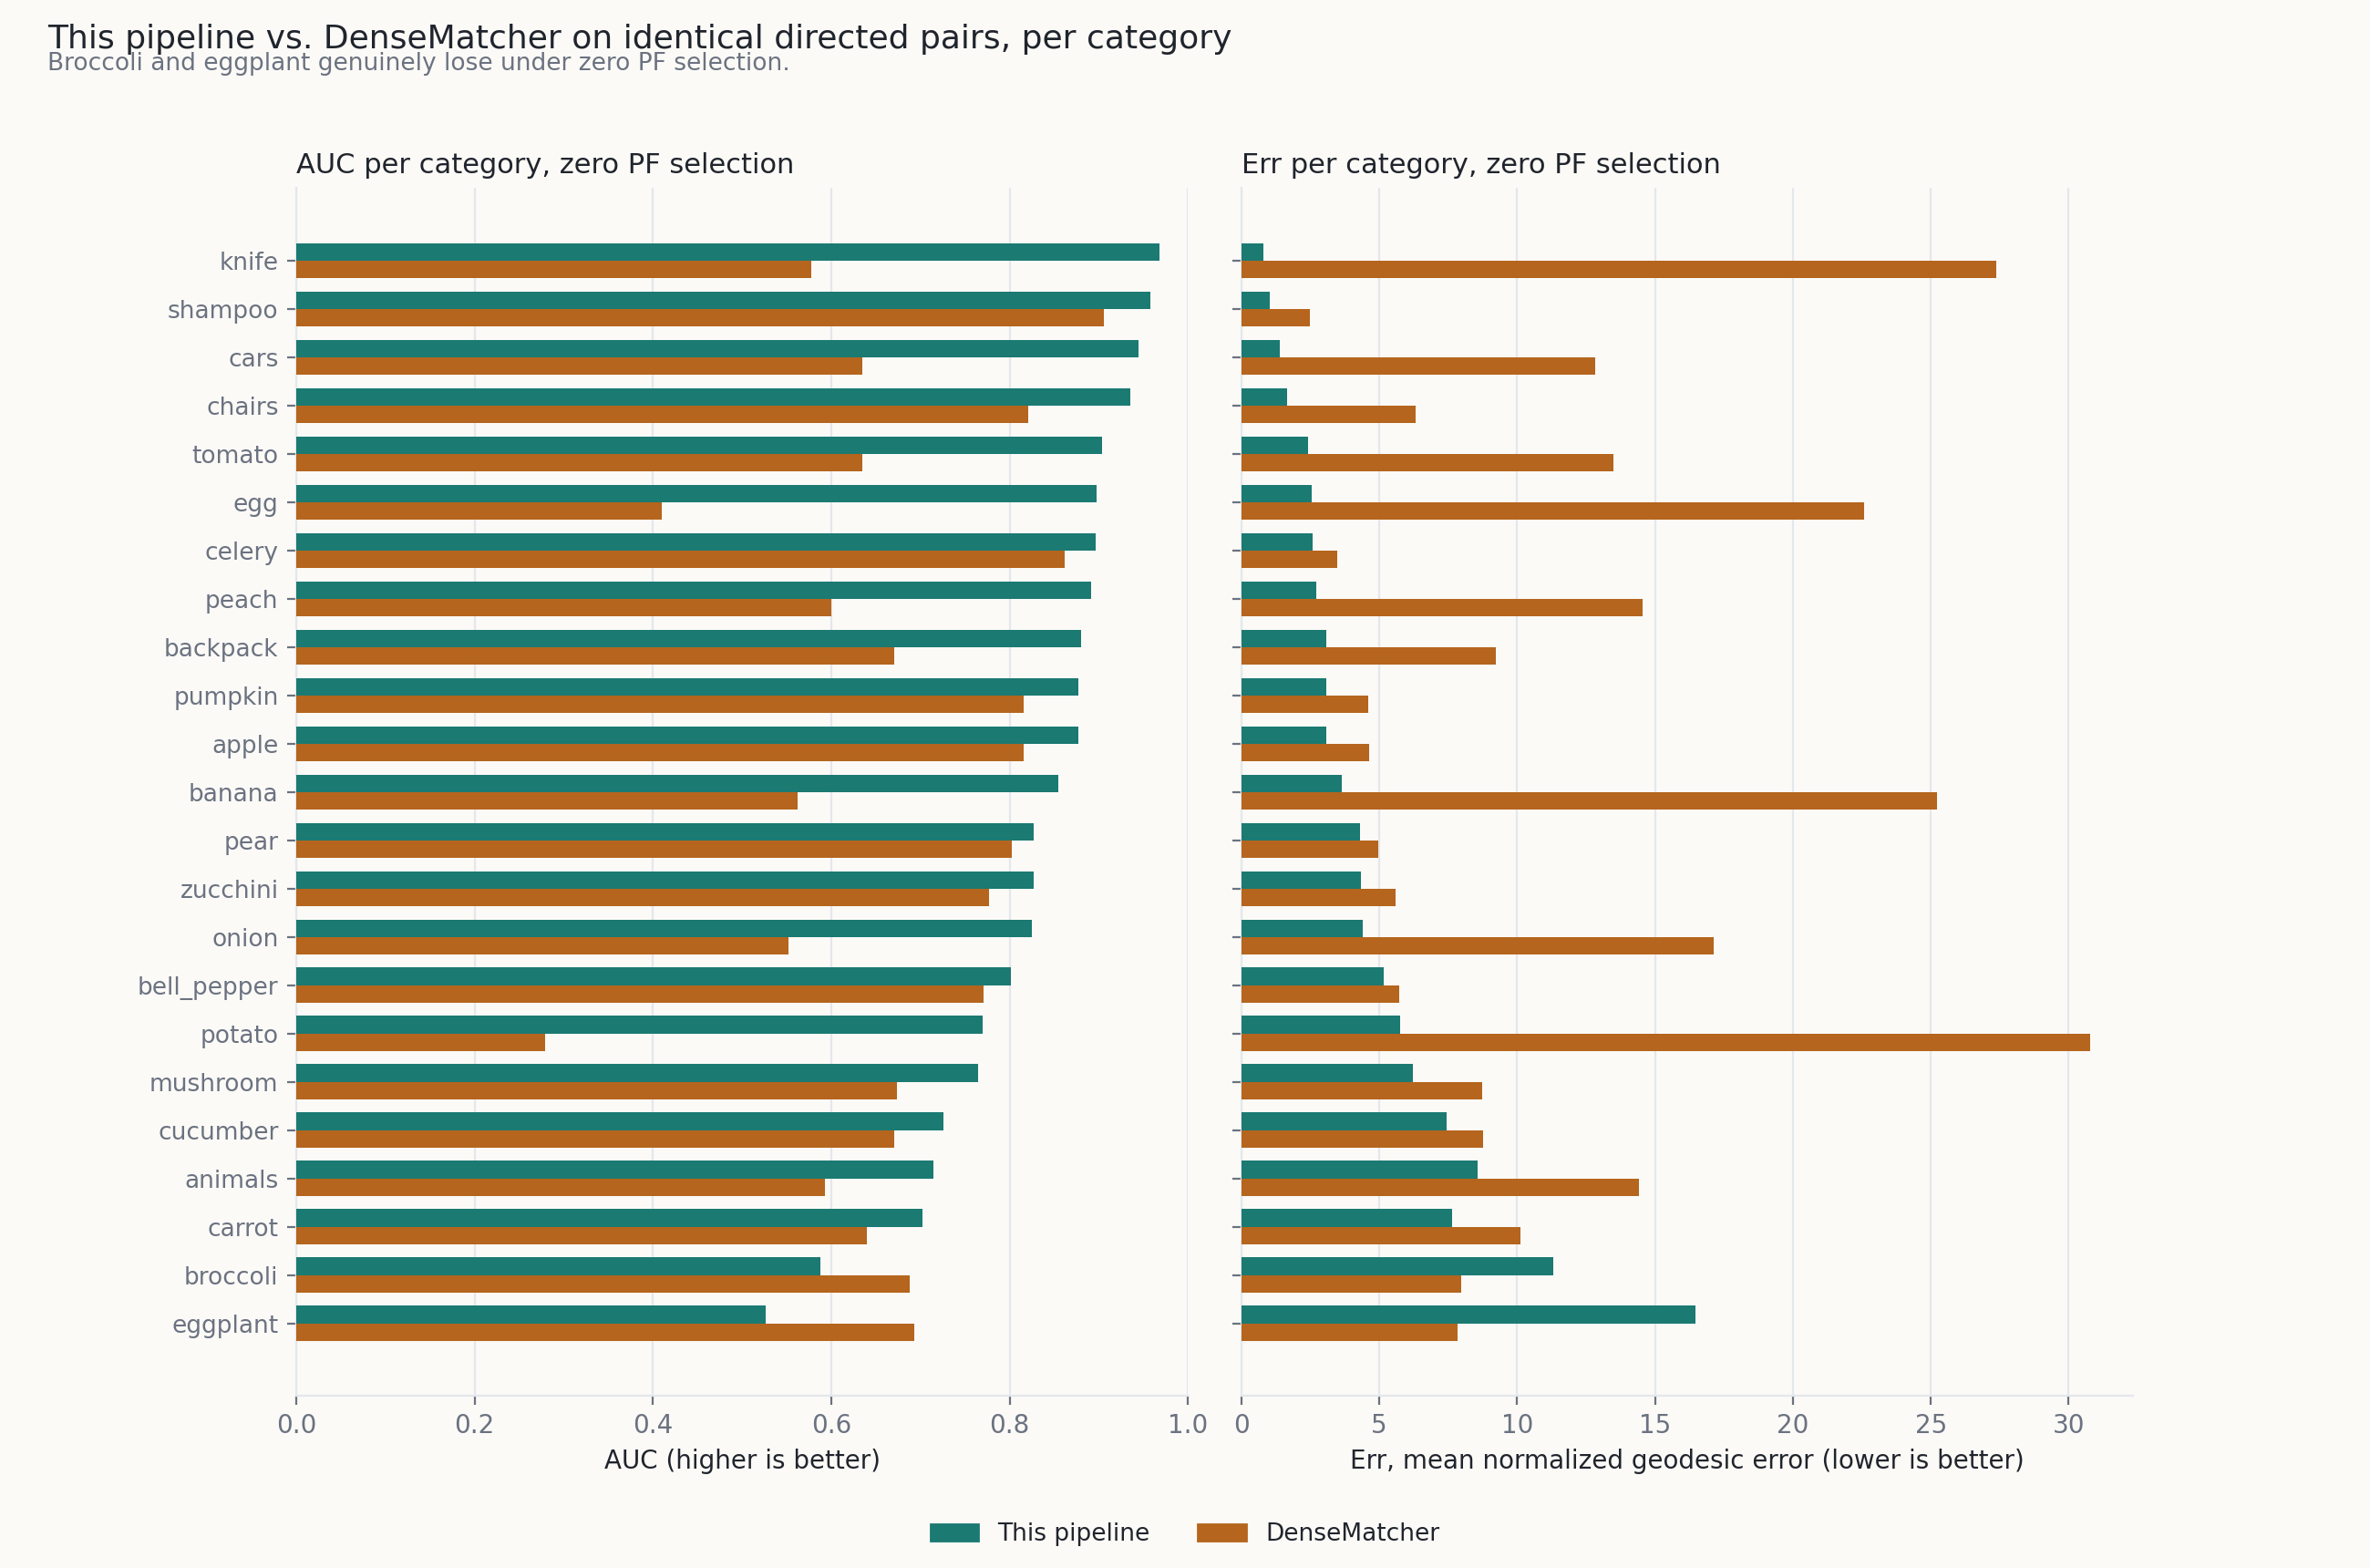
\includegraphics[width=0.98\textwidth]{figures/densematcher_category_comparison.png}
\caption{Per-category AUC and Err under range-averaged, zero-best-PF selection. Broccoli and
eggplant lose.}
\label{fig:densematcher-category}
\end{figure}

\subsection{Qualitative comparison: on the mesh}
\label{sec:densematcher-qualitative}

The numbers above compare correspondence quality; DenseMatcher itself only ever predicts a
per-vertex point correspondence (a functional map over DiffusionNet features refining multi-view
SD-DINO projections)~\cite{densematcher} and does not output a deformed mesh. To make it visually
comparable to this pipeline's output, the mesh that DenseMatcher's own predicted correspondence
implies gets rendered: the source mesh, unchanged in topology, with every vertex moved to the
position of its predicted match on the target -- exactly the lookup already used to score AUC/Err,
rendered here instead of only scored. Figure~\ref{fig:densematcher-coherence} shows this for four
clean-provenance pairs spanning the range of DenseMatcher failure severity actually measured:
knife (near-total failure, AUC $0.219$), potato (a severe failure, AUC $0.357$), cars (a milder
failure, AUC $0.469$), and shampoo (the mildest gap of the four, AUC $0.769$). Source vertices
carry a fixed position-based rainbow; Final and the DenseMatcher warp inherit it unchanged, since
both share the source mesh's vertex indices. A spatially coherent result keeps the rainbow smooth;
a confused correspondence scrambles it -- the standard texture-transfer diagnostic from the
shape-correspondence literature, applied here to both methods on equal footing.

\begin{figure}[H]
\centering
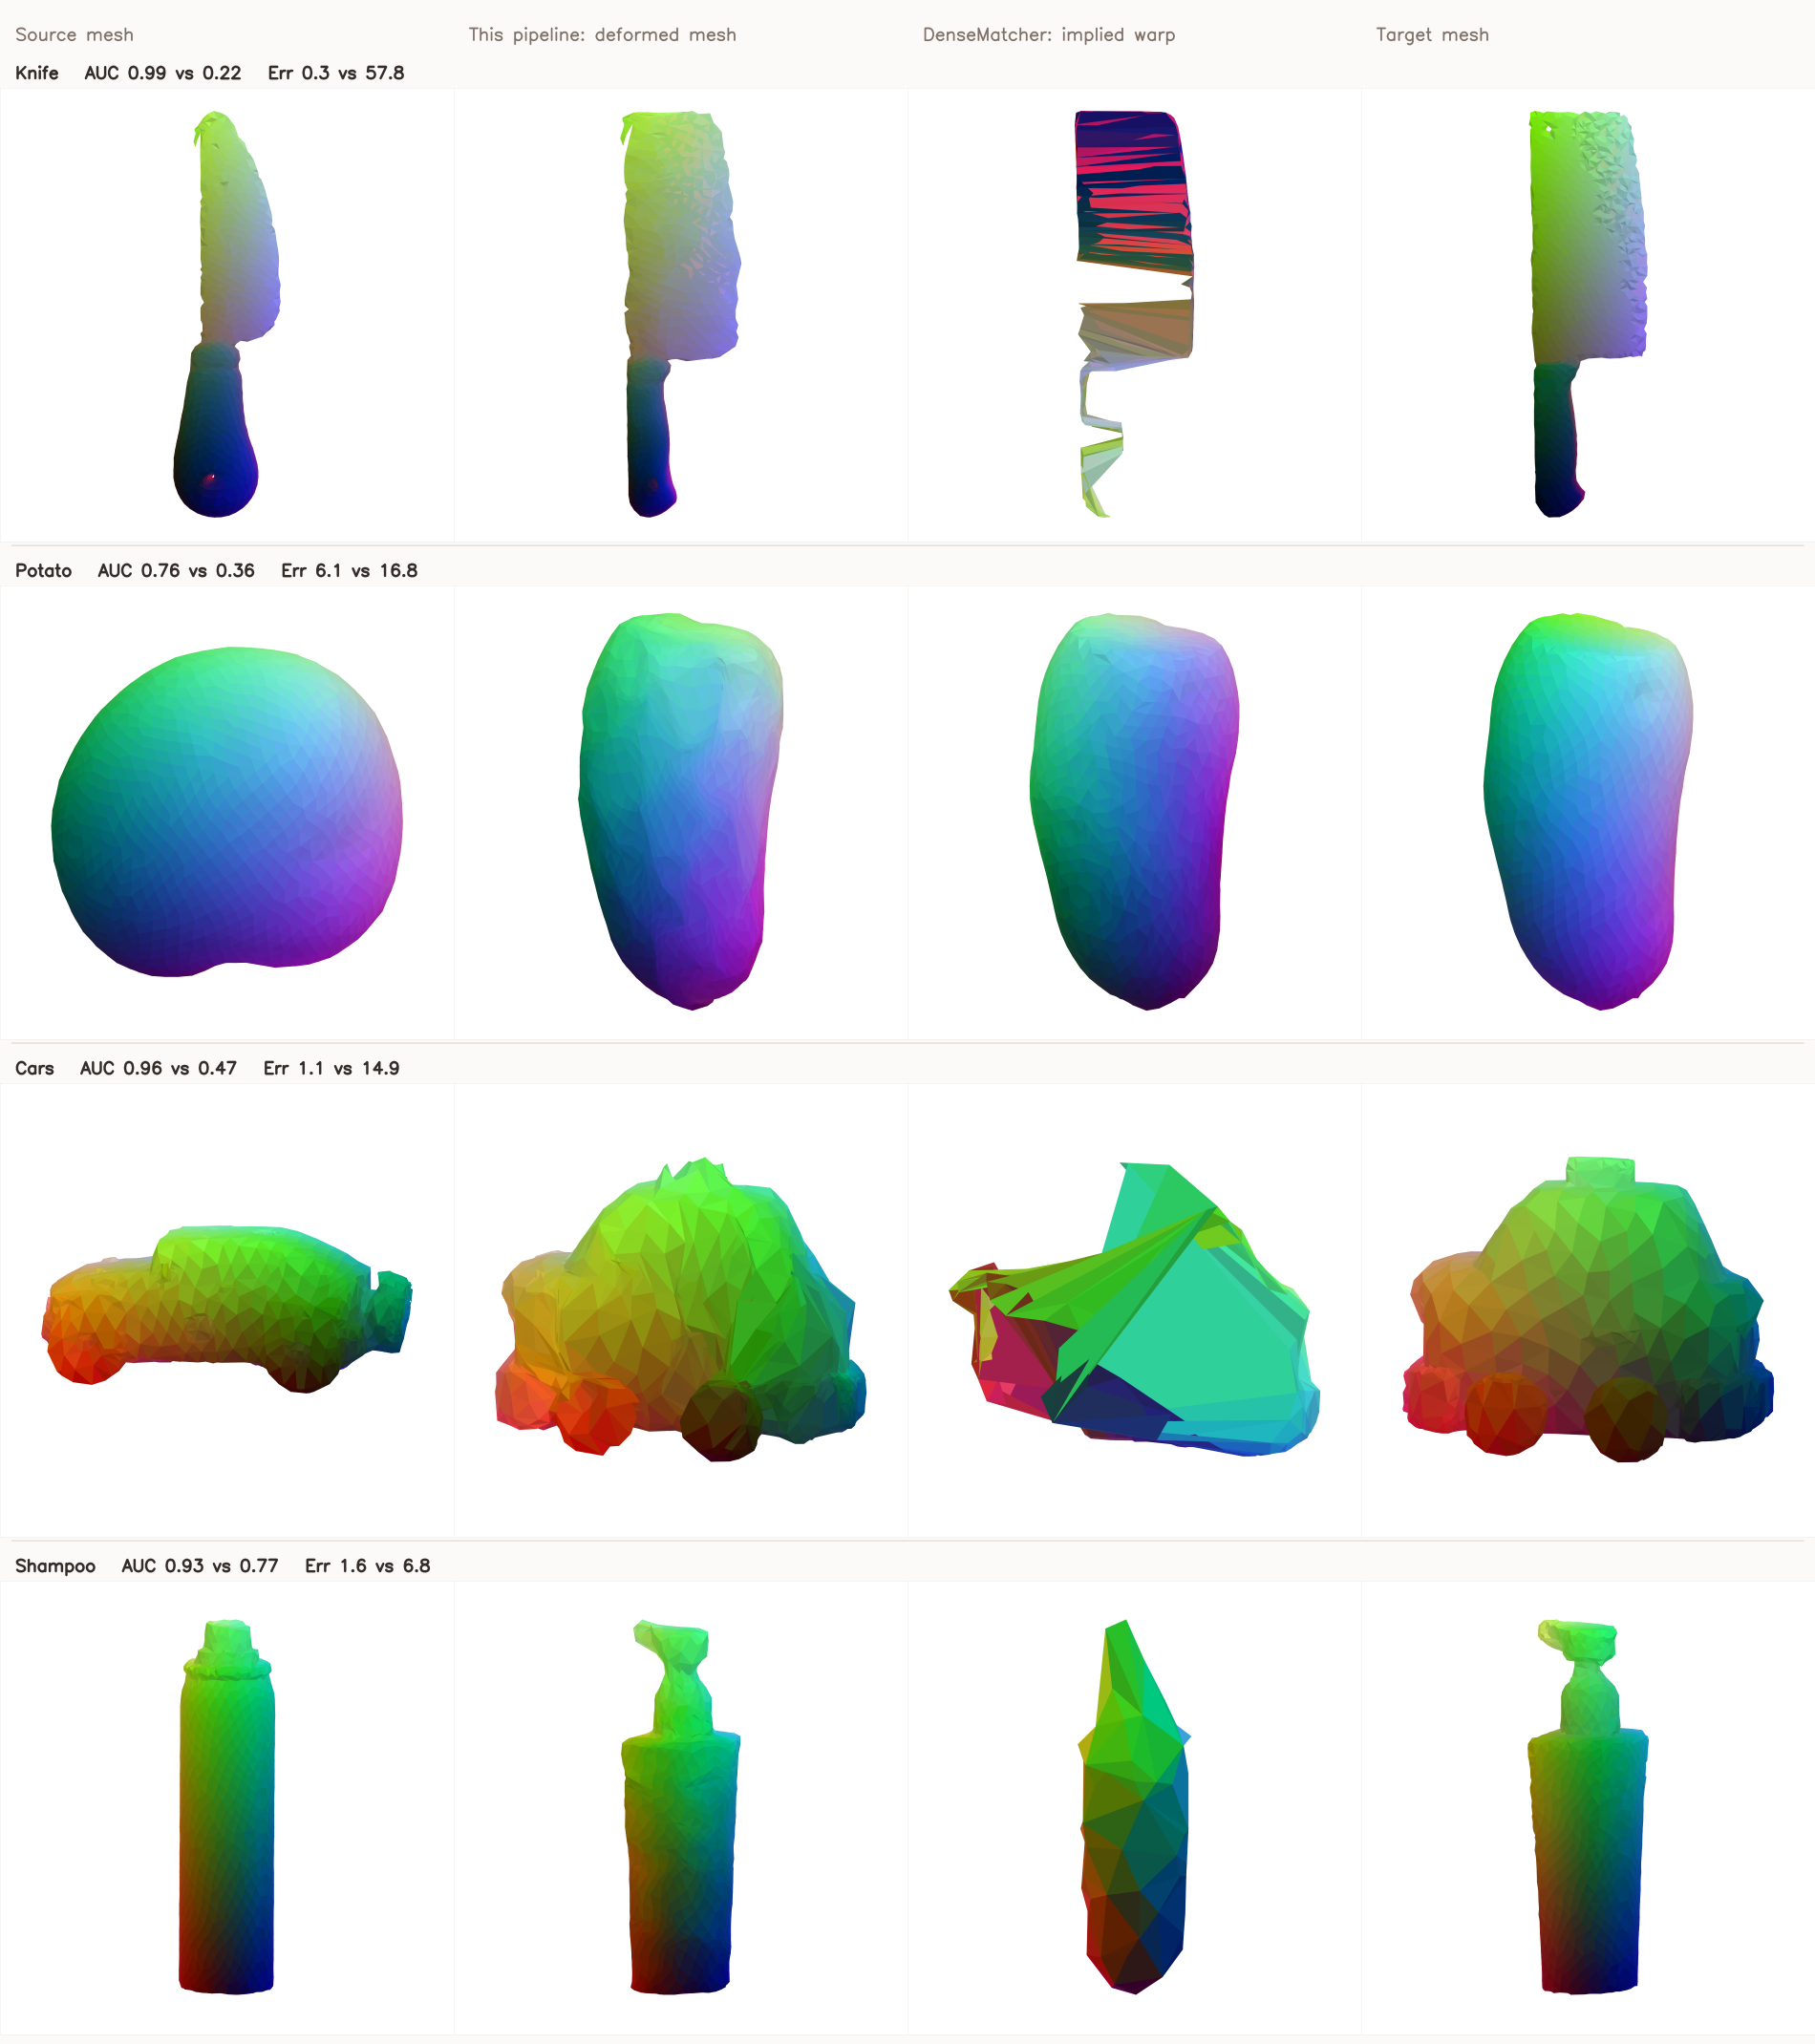
\includegraphics[width=0.98\textwidth]{figures/densematcher_deformation_coherence.png}
\caption{Source, Final, DenseMatcher's implied warp, and target, for four clean-provenance pairs.
Both warps inherit the source's rainbow coloring, so scrambling marks incoherence.}
\label{fig:densematcher-coherence}
\end{figure}

Figure~\ref{fig:densematcher-coherence}'s knife, cars, and shampoo rows visibly fold and
self-intersect under DenseMatcher's implied warp. Potato is the exception: despite the largest AUC
gap of the four, its warp stays smooth and blob-like -- less accurate, but not torn. This gap
between a summary statistic and the rendered geometry has a concrete explanation: AUC/Err
integrate partial credit over a normalized-geodesic threshold sweep, so a correspondence that is
uniformly somewhat wrong can post a similar AUC hit to one that is catastrophically wrong on a
smaller fraction of vertices, even though only the latter crushes the surface. Potato is the
former case; knife, cars, and shampoo are the latter.
% [ARTUR-FIX 4/9] Figure 8 lead-in + caption rephrased: illustrates the many-to-one failure mode, not a quantitative win.
Figure~\ref{fig:densematcher-distortion}
illustrates the mechanism behind that gap -- it is a diagnostic for the many-to-one failure
explained below, on four pairs chosen to span DenseMatcher's failure severity rather than to
represent typical performance, not a general quantitative benchmark -- with a topology-preserving
measure unrelated to AUC/Err: for every face, the
median $|\log_2(\text{deformed edge length} / \text{source edge length})|$, comparing the same
source edges under this pipeline's Final mesh and under DenseMatcher's implied warp. A value of
$0$ means a face moved rigidly; large values mean it was locally crushed or torn. On three of the
four pairs, DenseMatcher's implied warp is torn by two to nearly eight orders of magnitude more
than this pipeline's output; on potato, the two are comparable, confirming that its failure is a
smooth but systematically wrong correspondence rather than a torn one.

The concrete mechanism behind that tearing is a many-to-one correspondence: nothing forces
DenseMatcher's predicted map to be one-to-one, so several different source vertices are free to
land on the same (or a nearly identical) target vertex. Every edge between two such vertices then
collapses toward zero length, which is exactly what a large edge-distortion score is picking up.
This pipeline cannot fail this way by construction: it moves the source mesh's own vertices
directly, so its output always keeps the source's vertex count and connectivity, with no
correspondence step that could collapse several vertices onto one point.

\begin{figure}[H]
\centering
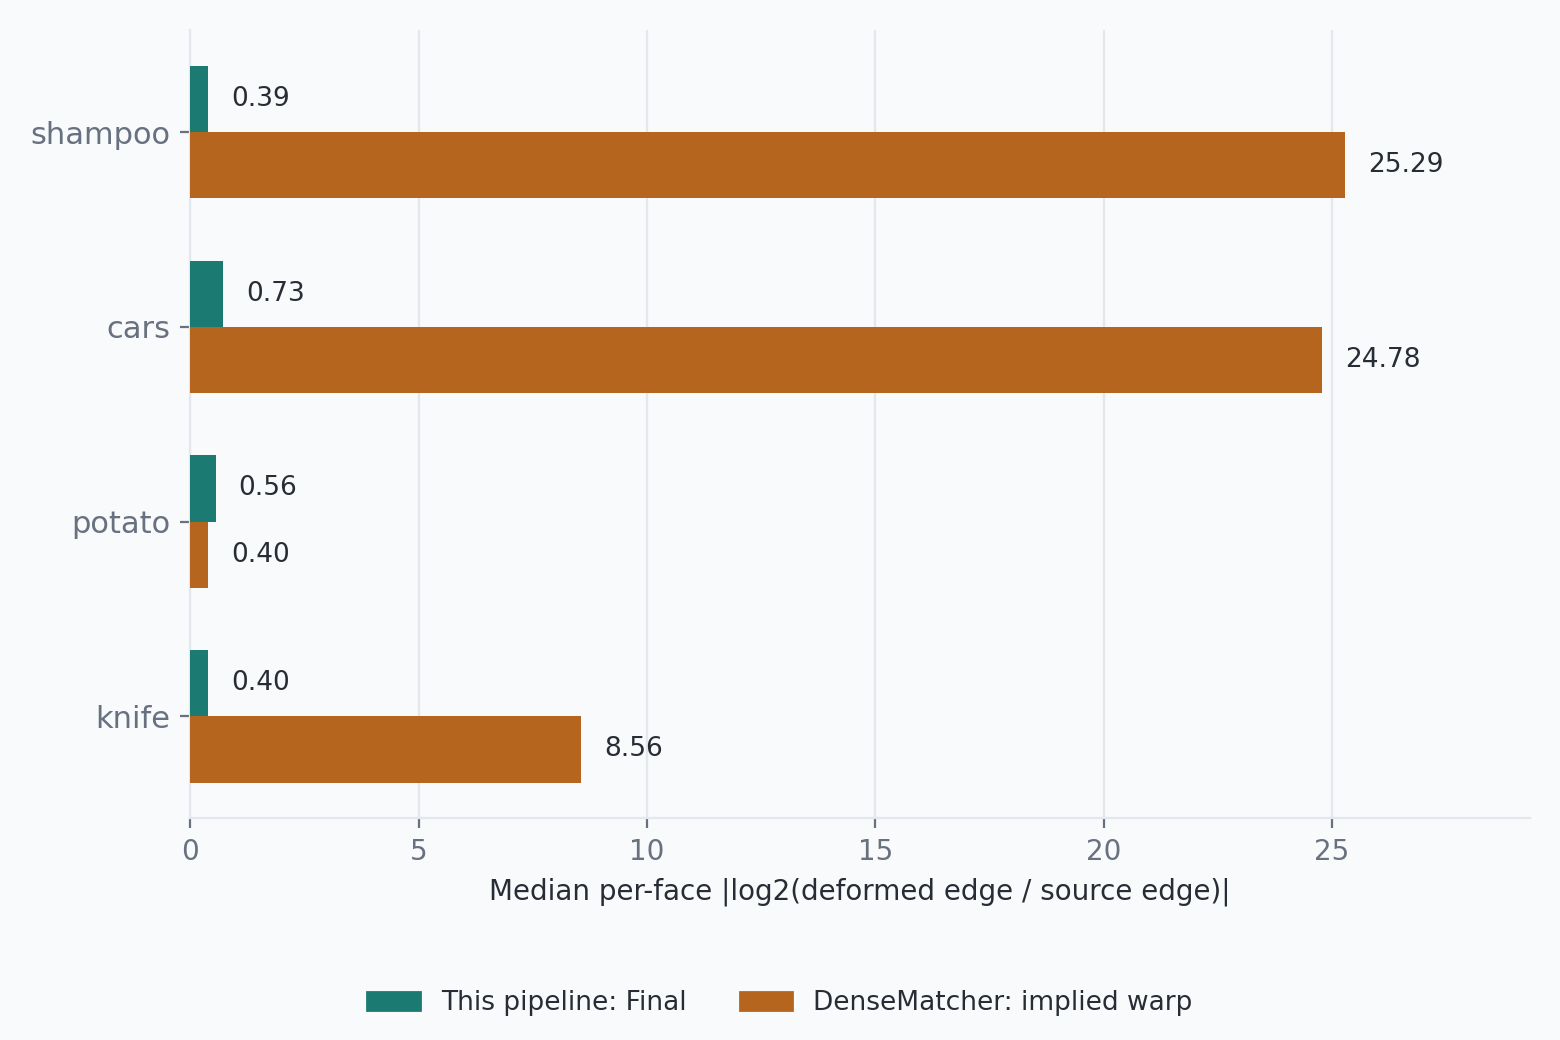
\includegraphics[width=0.75\textwidth]{figures/densematcher_edge_distortion_bars.png}
\caption{Median per-face local edge-stretch distortion for the same four pairs (linear scale),
illustrating the many-to-one correspondence failure described in the text rather than serving as a
general quantitative benchmark: these four pairs were chosen to span DenseMatcher's failure
severity, not sampled to represent typical performance. Lower is better.}
\label{fig:densematcher-distortion}
\end{figure}

\subsection{Full per-category table}

Table~\ref{tab:densematcher-full} also records input preparation. ``Clean'' means the category
used the canonical meshes directly or only label-free geometry/visual orientation checks.
``Assisted'' means additional preparation was needed to put source and target into comparable
orientations before PartField was applied.

\begingroup
\scriptsize
\setlength{\tabcolsep}{2.5pt}
\begin{longtable}{@{}l>{\raggedright\arraybackslash}p{1.75cm}rcrrrrl@{}}
\caption{Full per-category comparison under range-averaged, zero-best-PF selection. Rows are
evaluated (directed pair, PF-setting) entries, not unique directed pairs.}
\label{tab:densematcher-full}\\
\toprule
Category & \shortstack{Mesh\\prep} & Rows & PF range & \shortstack{Ours\\AUC} & \shortstack{Ours\\Err} & \shortstack{DM\\AUC} & \shortstack{DM\\Err} & Verdict \\
\midrule
\endfirsthead
\toprule
Category & \shortstack{Mesh\\prep} & Rows & PF range & \shortstack{Ours\\AUC} & \shortstack{Ours\\Err} & \shortstack{DM\\AUC} & \shortstack{DM\\Err} & Verdict \\
\midrule
\endhead
animals & clean & 180 & PF01--09 & 0.7148 & 8.578 & 0.5934 & 14.429 & win \\
apple & assisted & 80 & PF05--10 & 0.8770 & 3.078 & 0.8154 & 4.620 & win \\
backpack & clean & 60 & PF04--08 & 0.8805 & 3.063 & 0.6706 & 9.223 & win \\
banana & assisted & 120 & PF01--04 & 0.8546 & 3.639 & 0.5618 & 25.220 & win \\
bell\_pepper & assisted & 72 & PF01--04 & 0.8018 & 5.170 & 0.7712 & 5.726 & win \\
broccoli & clean & 120 & PF01--06 & 0.5875 & 11.313 & 0.6883 & 7.978 & \textbf{lose} \\
carrot & clean & 36 & PF02--04 & 0.7025 & 7.648 & 0.6404 & 10.132 & win \\
cars & clean & 100 & PF04--08 & 0.9449 & 1.397 & 0.6345 & 12.843 & win \\
celery & clean & 45 & PF01--06 & 0.8967 & 2.583 & 0.8615 & 3.464 & win \\
chairs & clean & 100 & PF04--08 & 0.9350 & 1.658 & 0.8212 & 6.329 & win \\
cucumber & clean & 120 & PF01--06 & 0.7255 & 7.426 & 0.6708 & 8.768 & win \\
egg & assisted & 150 & PF01--05 & 0.8977 & 2.562 & 0.4095 & 22.588 & win \\
eggplant & clean & 36 & PF01--06 & 0.5265 & 16.475 & 0.6927 & 7.847 & \textbf{lose} \\
knife & clean & 48 & PF02--05 & 0.9679 & 0.802 & 0.5780 & 27.370 & win \\
mushroom & assisted & 120 & PF01--04 & 0.7642 & 6.209 & 0.6734 & 8.724 & win \\
onion & assisted & 121 & PF01--06 & 0.8246 & 4.401 & 0.5523 & 17.125 & win \\
peach & assisted & 120 & PF01--05 & 0.8917 & 2.706 & 0.6000 & 14.559 & win \\
pear & clean & 120 & PF01--04 & 0.8275 & 4.313 & 0.8027 & 4.953 & win \\
potato & assisted & 80 & PF01--06 & 0.7701 & 5.754 & 0.2791 & 30.792 & win \\
pumpkin & assisted & 120 & PF02--07 & 0.8771 & 3.073 & 0.8163 & 4.599 & win \\
shampoo & clean & 80 & PF01--04 & 0.9584 & 1.043 & 0.9058 & 2.497 & win \\
tomato & assisted & 120 & PF01--07 & 0.9038 & 2.404 & 0.6348 & 13.481 & win \\
zucchini & assisted & 180 & PF01--06 & 0.8272 & 4.341 & 0.7767 & 5.588 & win \\
\bottomrule
\end{longtable}
\endgroup

% [ARTUR-FIX 2/9] New subsection + table: DenseMatcher's own published per-category numbers next to reimplemented ones.
\subsection{Published DenseMatcher numbers, where available}

DenseMatcher's paper does not publish a full 23-category breakdown; it reports only the aggregate
numbers already given above, plus one appendix table comparing against a single baseline (URSSM) on
four categories chosen for ``complex topologies''~\cite{densematcher}. Table~\ref{tab:densematcher-published}
reproduces that appendix table's DenseMatcher column next to both the reimplemented DenseMatcher
score from this report's own graph-geodesic evaluator and this pipeline's own score, for the four
categories where a published per-category number exists. These are not pair-matched the way the
rest of this section is -- DenseMatcher's appendix table does not state which exact objects or
directed pairs it averages over -- so this is a category-level sanity check on evaluator-protocol
differences, not a controlled comparison.

\begin{table}[H]
\centering
\small
\begin{tabular}{lrrr}
\toprule
Category & \shortstack{Pipeline Err\\(this report)} & \shortstack{DenseMatcher Err\\(reimplemented)} & \shortstack{DenseMatcher Err\\(published~\cite{densematcher})} \\
\midrule
Animals & 8.578 & 14.429 & 3.21 \\
Chairs & 1.658 & 6.329 & 3.51 \\
Broccoli & 11.313 & 7.978 & 3.06 \\
Shampoo & 1.043 & 2.497 & 3.15 \\
\bottomrule
\end{tabular}
\caption{DenseMatcher's own published per-category Err~\cite{densematcher} against this report's
reimplemented graph-geodesic score for DenseMatcher, for the four categories DenseMatcher's paper
reports individually. Lower is better. The published numbers are consistently lower (better) than
the reimplemented ones on three of four categories, and higher on shampoo -- evidence that evaluator
and protocol differences, not just method differences, separate this report's DenseMatcher numbers
from DenseMatcher's own published ones.}
\label{tab:densematcher-published}
\end{table}

The gap between DenseMatcher's published and reimplemented numbers is not uniform in direction,
which is itself informative: it is evidence against a simple ``the graph-geodesic evaluator is
unfair to DenseMatcher'' explanation, and consistent instead with the evaluator and protocol
differences already noted above (Dijkstra graph-geodesic distance rather than exact geodesic
distance, a different normalized-threshold convention that DenseMatcher's own paper does not fully
specify, and -- for categories outside the clean-preparation subset -- a different mesh
orientation).

\subsection{Mean vs.\ median diagnostic}

Under the same graph-geodesic scorer, DenseMatcher's released predictions have
a much heavier failure tail than their median alone suggests, while the pipeline's tested
granularities form a less skewed distribution.

\begin{table}[H]
\centering
\small
\begin{tabular}{lrrrr}
\toprule
& Pipeline AUC & Pipeline Err & DenseMatcher AUC & DenseMatcher Err \\
\midrule
Pooled diagnostic & & & & \\
\quad Mean & 0.8255 & 4.659 & 0.6632 & 12.089 \\
\quad Median & 0.8627 & 3.444 & 0.7464 & 6.410 \\
\bottomrule
\end{tabular}
\caption{Mean vs.\ median AUC/Err. Pipeline values pool 2328 (directed pair, PF-setting) rows;
DenseMatcher values pool 496 unique directed pairs, so this is a tail diagnostic rather than the
headline fairness claim.}
\label{tab:mean-median}
\end{table}

\section{Surface Quality}
\label{sec:surface-quality}

% [ARTUR-FIX 7/9] Removed the unsupported "geometrically clean" claim; reformulated to state only what is actually measured.
Dense correspondence metrics ask whether semantic regions match. They do not by themselves say
whether the final mesh stays close to the target surface and keeps smooth, locally consistent
geometry. For that reason the project also
evaluates surface quality using symmetric Chamfer, \Fscore{}, robust $p95$ surface distance, normal
consistency, and semantic-region versions of Chamfer and F-score, computed in a unit-box
coordinate system so numbers are comparable across objects of different original scale. These are
proximity and smoothness proxies, not a direct count of mesh-validity failures such as
self-intersections or flipped triangles: this report does not measure those numerically, and
instead controls for them during optimization through the regularizers in
Section~\ref{sec:loss-function} and inspects for them qualitatively through the figures and video
showcases referenced throughout (Section~\ref{sec:failure-modes} discusses the cases where they
appear). In this
normalization, a threshold of $0.02$ is strict: it asks for surface samples to be very close
relative to the whole object.

This section reports the \emph{extended} surface-quality evaluation: in
addition to the original $4$ SAM3D animal pairs and $2$ cross-dataset chain pairs, $4$ more SAM3D
animal pairs (Cat$\to$Chihuahua, Cat$\to$Fox, Goldie$\to$Fox, Goldie$\to$Pug). No DenseCorr3D
ground truth exists for any of these self-created meshes, so only geometric surface metrics are
reported, not AUC/Err.

\begin{table}[H]
\centering
\small
\begin{tabularx}{\textwidth}{Xrrrrrr}
\toprule
Experiment family & $n$ & \Chamfer{} $\downarrow$ & \Fscore{} $\uparrow$ & $p95$ $\downarrow$ & Normal $\uparrow$ & \shortstack{Sem.\\ \Fscore{} $\uparrow$} \\
\midrule
SAM3D animal pairs & 8 & 0.0223 & 0.9354 & 0.0212 & 0.9411 & 0.9142 \\
Cross-dataset chain examples & 2 & 0.0210 & 0.9304 & 0.0236 & 0.8805 & 0.9104 \\
SAM3D vehicle pairs & 5 & 0.0343 & 0.7033 & 0.0334 & 0.8585 & 0.6740 \\
DenseCorr3D fair all-animal best-PF stress test & 90 & 0.0568 & 0.4724 & 0.1000 & 0.8284 & 0.4525 \\
\bottomrule
\end{tabularx}
\caption{Surface quality in unit-box coordinates, extended evaluation. Vehicles
are markedly weaker than animals under the identical \texttt{pfonly} recipe.}
\label{tab:surface-aggregate}
\end{table}

The animal pairs have mean \Chamfer{} $0.0223$ and mean \Fscore{} $0.935$: the final deformed
surfaces closely cover the target surfaces, and semantic \Fscore{} ($0.914$) tracks the global score
closely, meaning the good fit is not only produced by one large body region covering the target.
The vehicle pairs, run with the exact same PartField-only recipe, are clearly weaker: mean
\Fscore{} drops to $0.703$ and semantic \Fscore{} to $0.674$.

\begin{figure}[H]
\centering
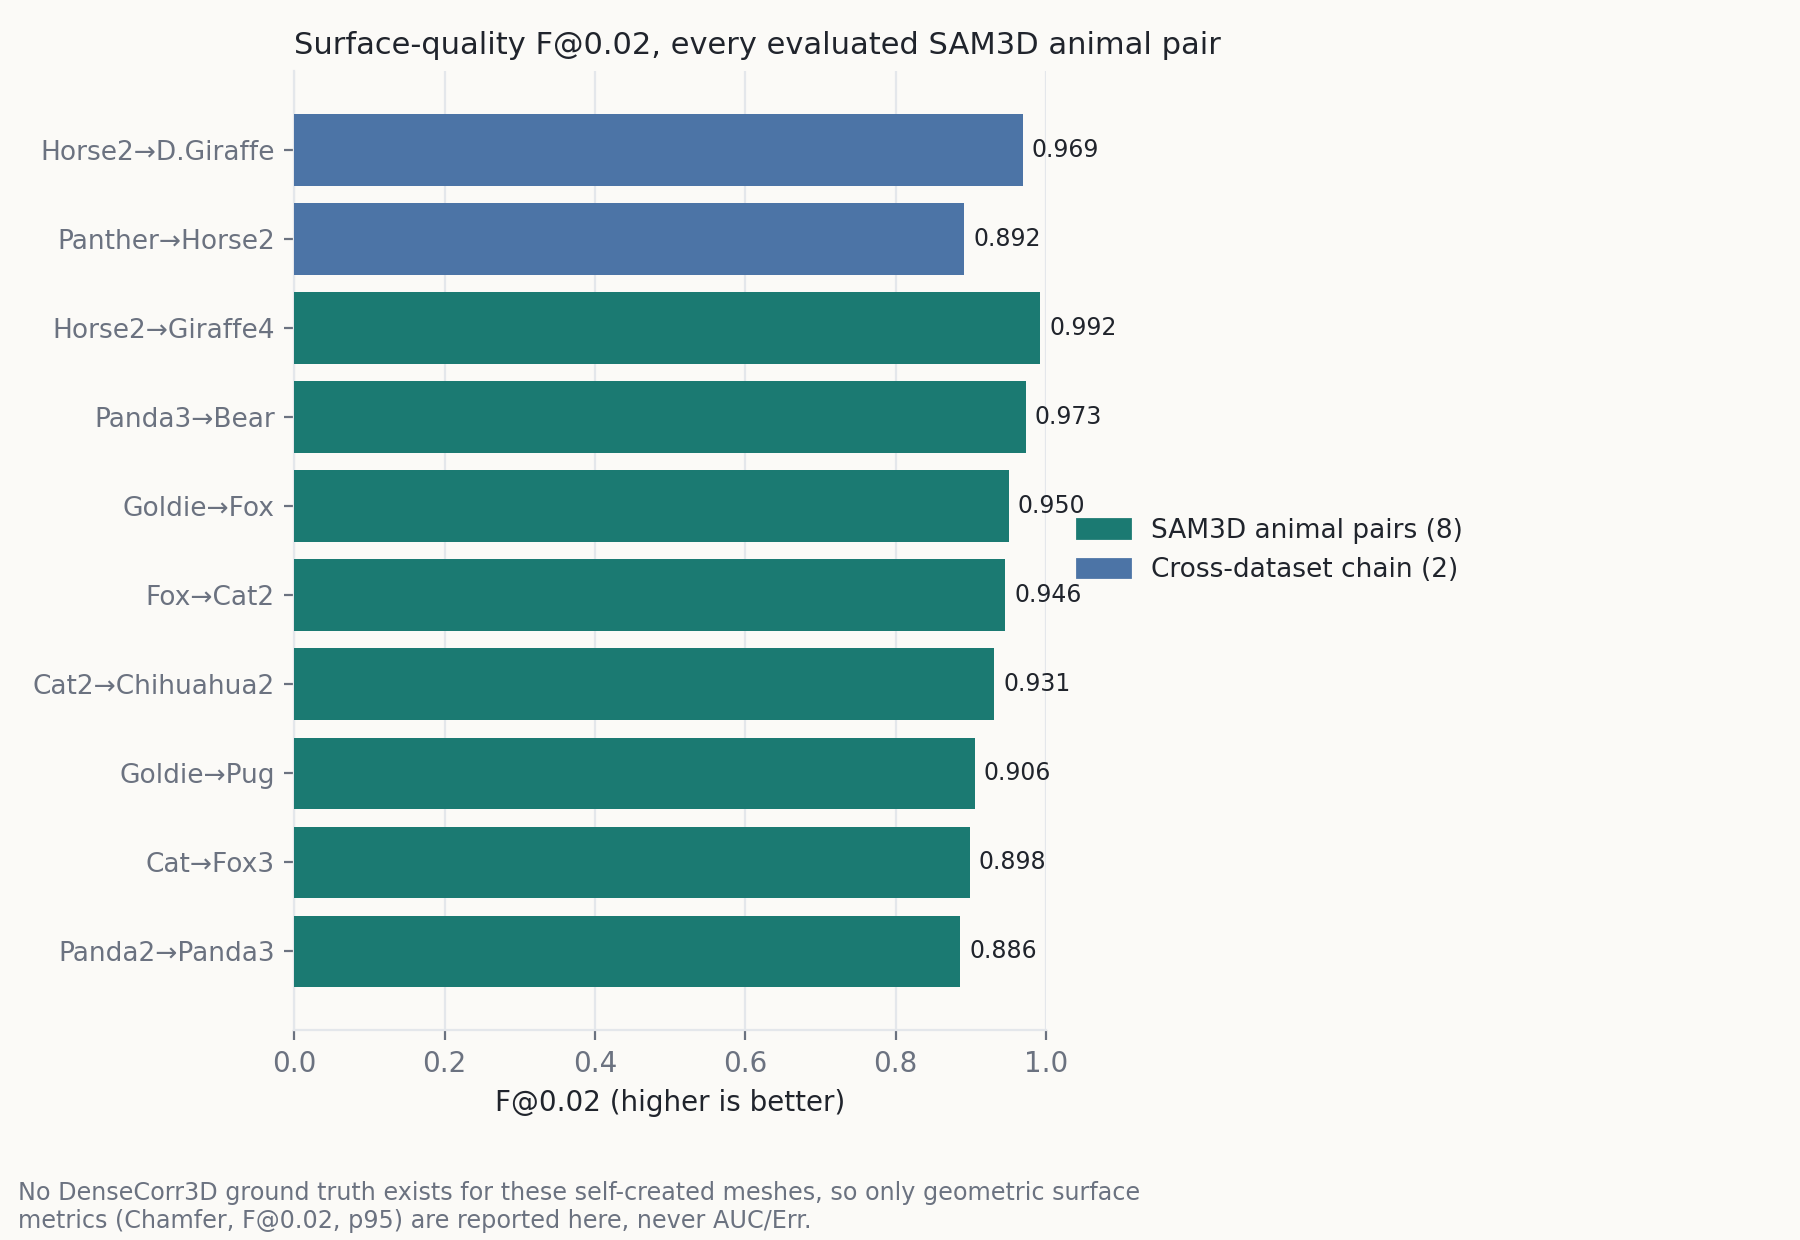
\includegraphics[width=0.86\textwidth]{figures/sam3d_extended_fscore.png}
\caption{F@0.02 for SAM3D animal and cross-dataset chain pairs.}
\label{fig:sam3d-extended}
\end{figure}

\begin{table}[H]
\centering
\small
\begin{tabularx}{\textwidth}{lrrrrr}
\toprule
Run & \Chamfer{} $\downarrow$ & \Fscore{} $\uparrow$ & $p95$ $\downarrow$ & Sem.\ \Chamfer{} $\downarrow$ & Sem.\ \Fscore{} $\uparrow$ \\
\midrule
Horse2 $\rightarrow$ Giraffe4 & 0.0134 & 0.9923 & 0.0129 & 0.0141 & 0.9836 \\
Panda3 $\rightarrow$ Bear & 0.0199 & 0.9730 & 0.0183 & 0.0210 & 0.9556 \\
Goldie $\rightarrow$ Fox & 0.0228 & 0.9503 & 0.0203 & 0.0239 & 0.9306 \\
Fox $\rightarrow$ Cat2 & 0.0224 & 0.9460 & 0.0209 & 0.0232 & 0.9333 \\
Cat2 $\rightarrow$ Chihuahua2 & 0.0246 & 0.9312 & 0.0242 & 0.0281 & 0.9058 \\
Goldie $\rightarrow$ Pug & 0.0248 & 0.9056 & 0.0236 & 0.0283 & 0.8732 \\
Cat $\rightarrow$ Fox3 & 0.0243 & 0.8985 & 0.0244 & 0.0259 & 0.8818 \\
Panda2 $\rightarrow$ Panda3 & 0.0261 & 0.8859 & 0.0251 & 0.0288 & 0.8495 \\
\midrule
Horse2 $\rightarrow$ Dense Giraffe (chain) & 0.0189 & 0.9692 & 0.0189 & 0.0209 & 0.9440 \\
Panther $\rightarrow$ Horse2 (chain) & 0.0231 & 0.8916 & 0.0283 & 0.0243 & 0.8769 \\
\midrule
Pink Smart $\rightarrow$ Red Smart & 0.0290 & 0.8196 & 0.0269 & 0.0310 & 0.7869 \\
F1 car $\rightarrow$ Verstappen & 0.0336 & 0.7275 & 0.0364 & 0.0354 & 0.7024 \\
Mini Cooper $\rightarrow$ Pink Smart & 0.0348 & 0.6709 & 0.0329 & 0.0370 & 0.6420 \\
Red truck1 $\rightarrow$ Red truck3 & 0.0379 & 0.6719 & 0.0371 & 0.0405 & 0.6441 \\
G-class $\rightarrow$ Green SUV & 0.0364 & 0.6268 & 0.0336 & 0.0390 & 0.5946 \\
\bottomrule
\end{tabularx}
\caption{Detailed surface-quality results, sorted within each group by \Fscore{}.}
\label{tab:sam3d-detail}
\end{table}

The best case overall remains Horse2 $\rightarrow$ Giraffe4, with \Chamfer{} $0.0134$ and \Fscore{}
$0.9923$: two compatible quadruped structures where PartField separates the main body regions
cleanly. The hardest animal case is Panda2 $\rightarrow$ Panda3, a same-species pair where the lower
\Fscore{} and higher semantic Chamfer reflect round body regions and pose differences reducing
precision.

\begin{figure}[H]
\centering
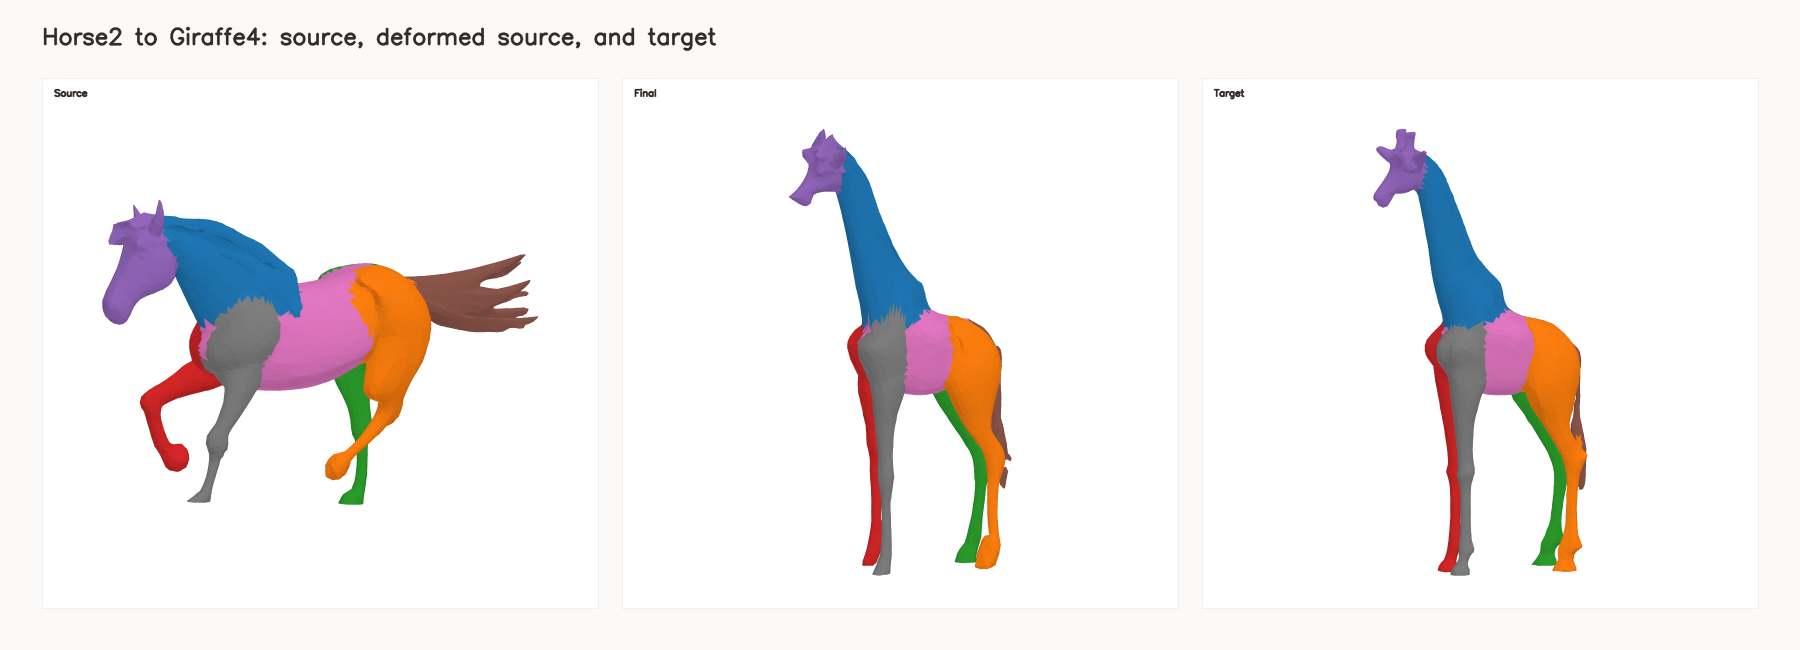
\includegraphics[width=0.86\textwidth]{figures/qual_horse2_to_giraffe4_grid.png}
\caption{Horse2 $\rightarrow$ Giraffe4: a compatible large-proportion deformation.}
\label{fig:qual-horse-giraffe}
\end{figure}

\begin{figure}[H]
\centering
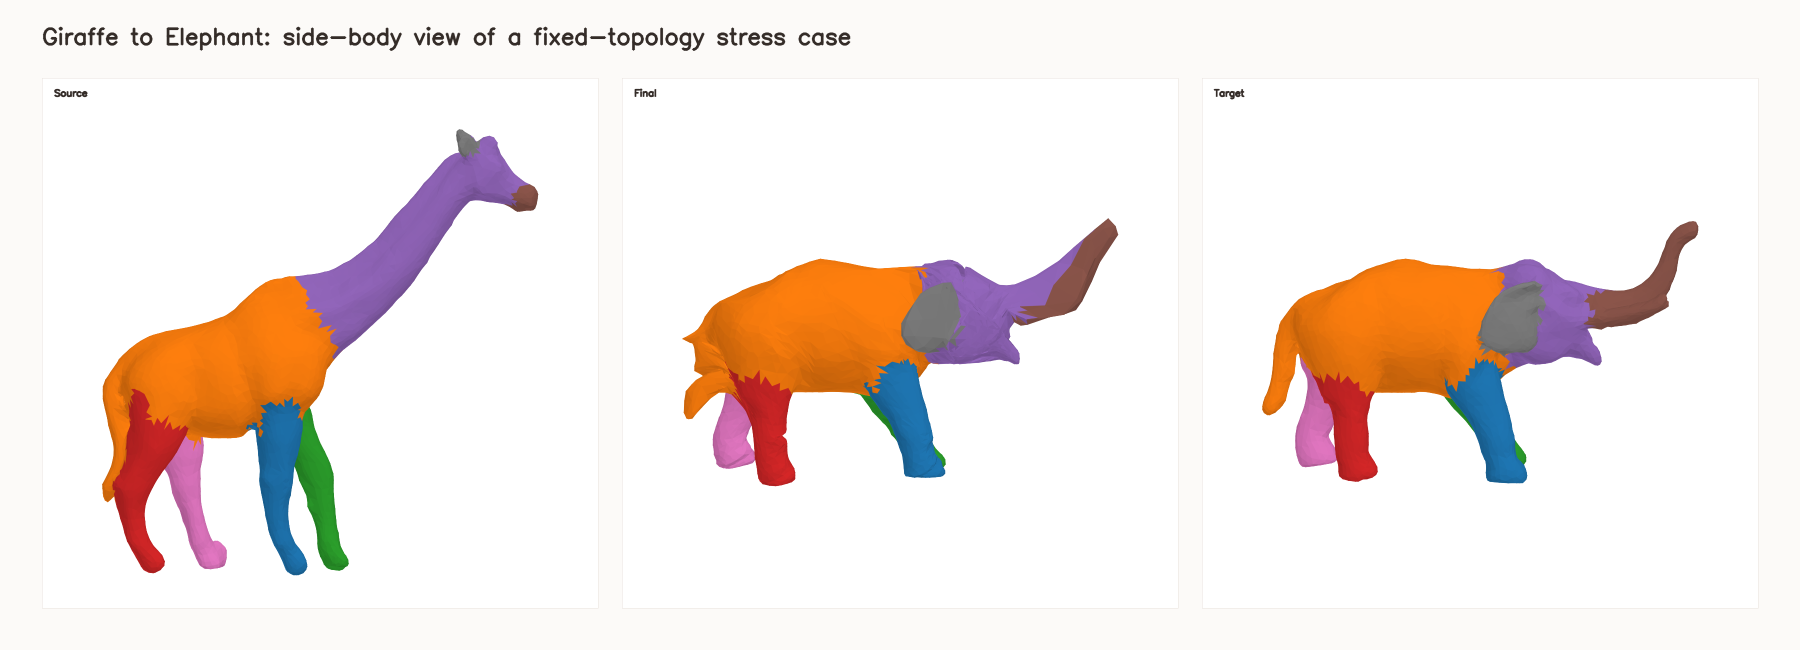
\includegraphics[width=0.86\textwidth]{figures/qual_giraffe_to_elephant_grid.png}
\caption{Giraffe $\rightarrow$ Elephant: hard topology transfer with missing trunk structure.}
\label{fig:qual-giraffe-elephant}
\end{figure}

\begin{figure}[H]
\centering
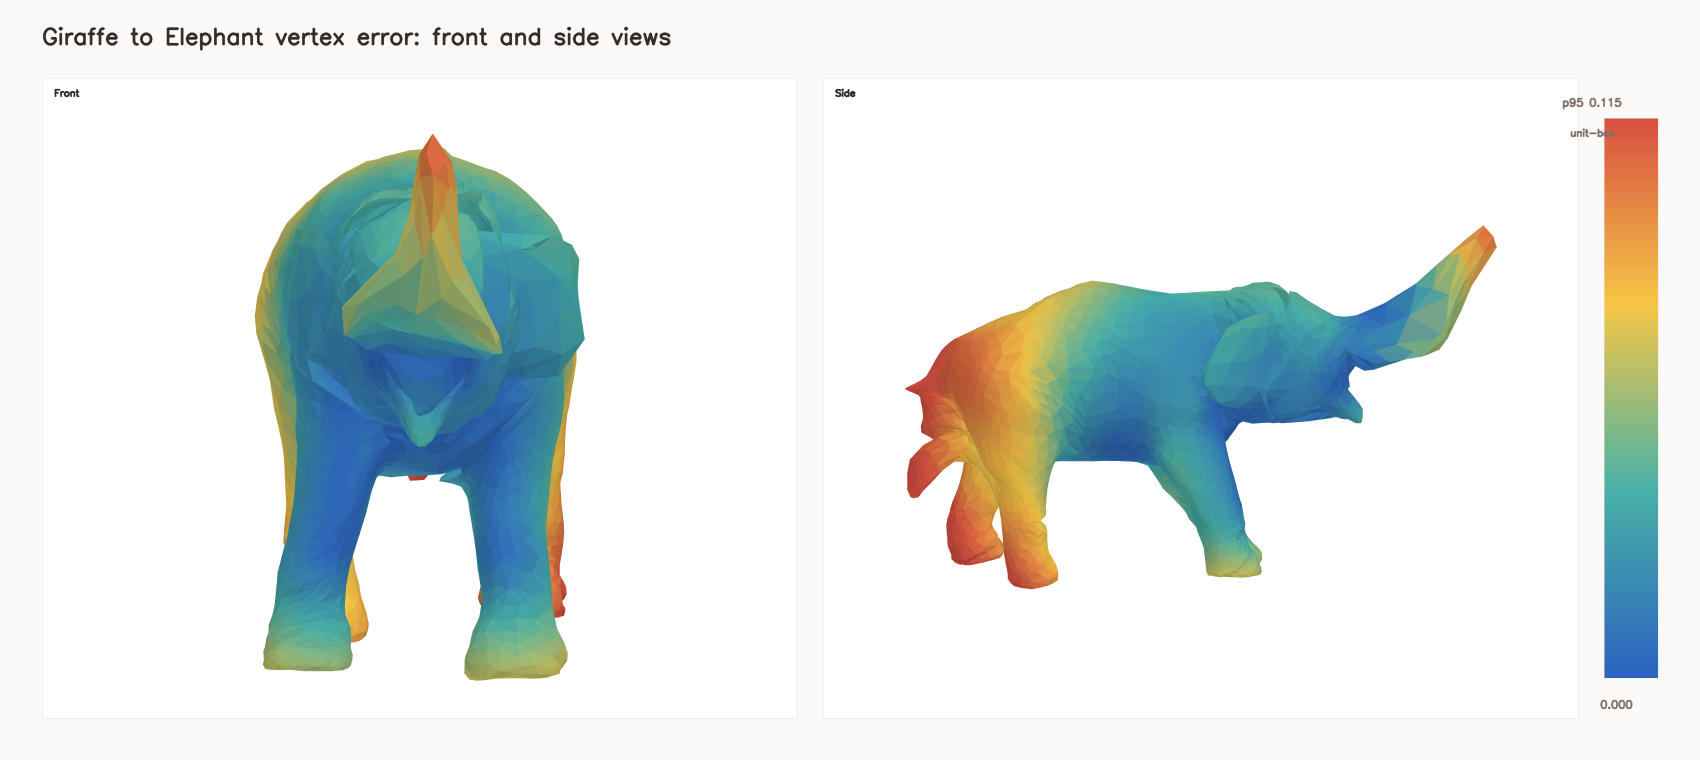
\includegraphics[width=0.86\textwidth]{figures/failure_vertex_heatmap.png}
\caption{Failure heatmap for Giraffe $\rightarrow$ Elephant. Color is nearest-target vertex
distance in unit-box coordinates, clipped at the run's $p95$ value shown on the colorbar.}
\label{fig:failure-heatmap}
\end{figure}

\begin{figure}[H]
\centering
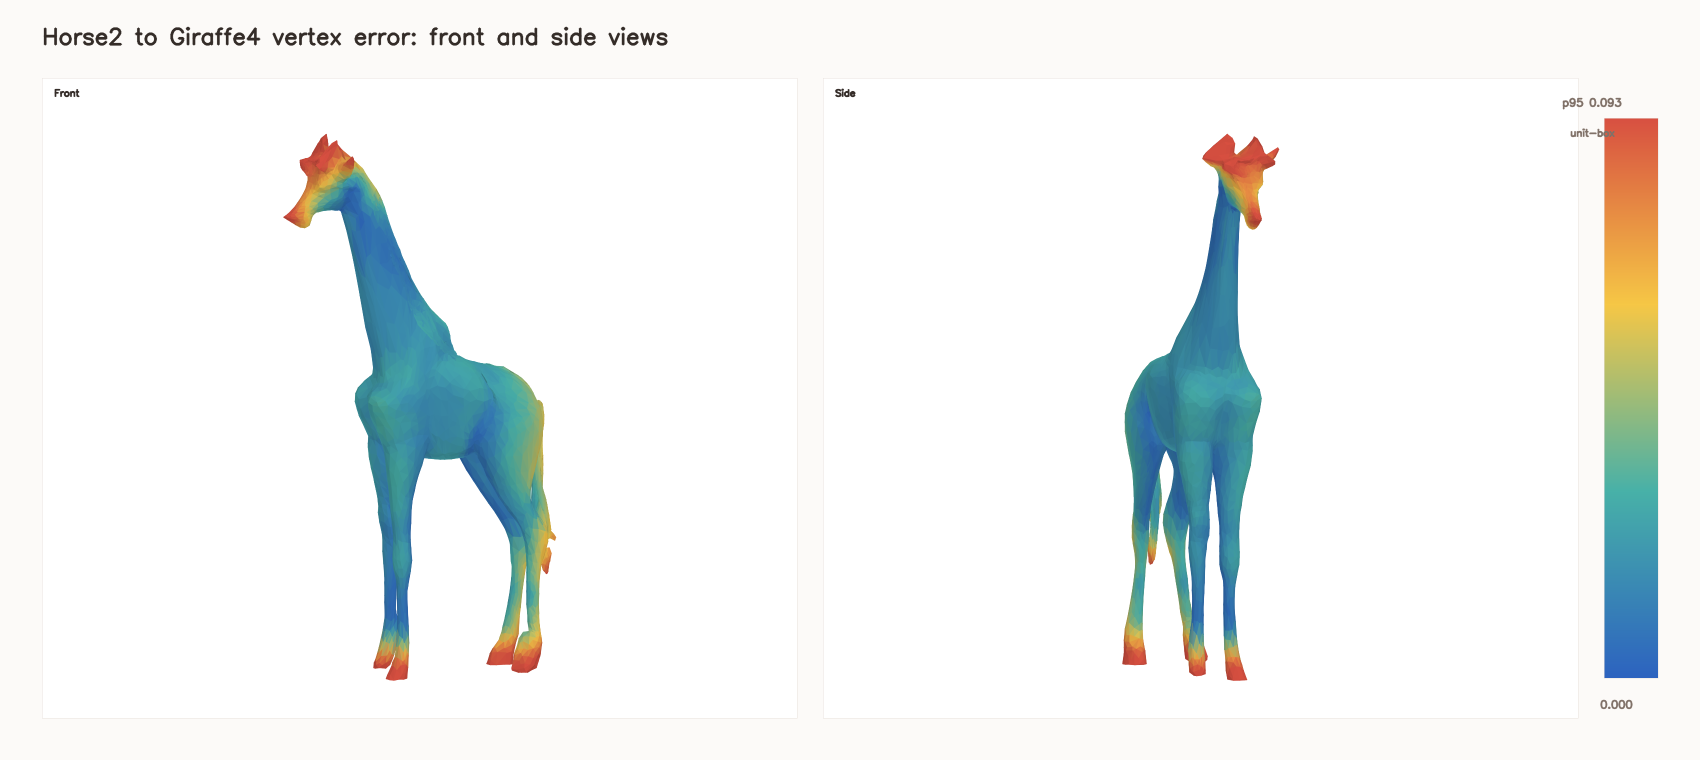
\includegraphics[width=0.86\textwidth]{figures/good_vertex_heatmap_horse2_giraffe4.png}
\caption{Heatmap for the successful Horse2 $\rightarrow$ Giraffe4 case. Color is nearest-target
vertex distance in unit-box coordinates, clipped at the run's $p95$ value shown on the colorbar.}
\label{fig:good-heatmap}
\end{figure}

\section{Cross-Category DenseCorr3D Experiments}

This section presents a root-cause diagnosis for the two categories that still lose against
DenseMatcher even in the fair, same-evaluator comparison of Section~\ref{sec:densematcher-fair}:
eggplant and broccoli. The same pattern is visible at a glance in
Figure~\ref{fig:densematcher-category}: categories with reliable, repeated parts perform best
(knife, shampoo, cars, chairs), while categories with weak part structure or strong intra-class
variation are much harder (broccoli, potato, eggplant).

\subsection{Root-cause diagnosis: why eggplant and broccoli lose}
\label{sec:root-cause}

Eggplant and broccoli are the two categories that still lose against DenseMatcher in the fair
comparison (Section~\ref{sec:densematcher-fair}), and each has a distinct, identifiable cause.

Eggplant's \texttt{groups.txt} divides the mesh into roughly $29$ thin rings running along its long
axis rather than coarse parts (group-axis correlation $-0.996$ with the mesh's principal axis, mean
ring extent only about $0.10$ of the object's length), and PartField's own unsupervised clusters do
not track these rings either, so the local Chamfer term has no reliable ring-level anchor to lock
onto.

Broccoli's failure has a different cause. Its \texttt{groups.txt} follows the crown's irregular,
branching floret structure, which PartField's unsupervised clustering does not recover: the buckets
it finds do not line up with the florets DenseCorr3D's annotators used, so the local Chamfer term
has no reliable structure to guide it.

Appendix~\ref{app:additional-qualitative} includes additional produce and hammer examples. They are
useful qualitative checks, but they are secondary to the main root-cause diagnosis here.

\section{Failure Modes}
\label{sec:failure-modes}

In this project, most bad results fall into a small number of categories: topology mismatch,
unstable buckets, orientation or pose mismatch, and metric sensitivity.

\begin{table}[H]
\centering
\small
\begin{tabularx}{\textwidth}{lXX}
\toprule
Failure mode & Symptom & Typical response \\
\midrule
Topology mismatch & Target contains structure the source cannot represent. & Use topology-aware methods or choose more compatible pairs. \\
Bucket instability & Local loss pulls a source part toward the wrong target region. & Try different PF levels, bucket balancing, or learned bucket matching. \\
Orientation mismatch & Buckets are swapped or mirrored before optimization starts. & Add canonical orientation and symmetry handling. \\
Pose mismatch & Limbs or protrusions begin in incompatible positions. & Use staged alignment or pose-aware preprocessing. \\
Metric tail failure & Mean score looks acceptable but $p95$ is large. & Inspect heatmaps and per-bucket errors rather than only averages. \\
\bottomrule
\end{tabularx}
\caption{Summary of the main failure modes observed in the project.}
\label{tab:failure-summary}
\end{table}

\subsection{Topology mismatch}

The deformation keeps the source topology. This is often desirable because it preserves a clean
mapping from original source vertices to deformed vertices. It is also a limitation. A horse can be
stretched toward a giraffe, but it cannot truly grow a new topological structure. An elephant trunk,
antlers, separated ears, or missing limbs must be approximated using existing source surface area,
producing the characteristic failure where the target is globally covered but one semantic part is
stolen from a neighboring region.

A smaller but very visible example appears in dog pairs such as Goldie $\rightarrow$ Pug. The tail
tips may be in different positions, and the tip of the source tail does not reliably follow the tip
of the target tail: a point-to-point correspondence method could explicitly say that one tail
endpoint should match the other, while a PartField bucket mainly says that a tail or rear-body
region should match another region, so exact endpoint identity can be lost.
Figure~\ref{fig:goldie-pug-tail} makes this concrete by tracking actual vertices rather than
buckets. Every vertex is colored by its own rest-pose position (the project's own position-color
scheme, \path{semantic_tracking/vertex_color_tracking.py}: RGB from per-axis normalized XYZ), so
the whole body, including the tail's own shape, is legible at a glance rather than reduced to a
single highlighted patch on a flat body. On top of that gradient, the farthest-out $30\%$ of the
source tail bucket is marked in bright yellow on the undeformed Goldie; because the deformation
preserves vertex correspondence exactly, the deformed mesh inherits the identical per-vertex
colors, so the same yellow patch shows precisely where that geometry physically ends up -- not on
the pug's own tail, but pulled onto the flank, near the hip. The pug's own tail tip (found the
same way, from its own bucket labels, and colored by its own independent position gradient) is
marked yellow on the target as well, so the comparison is the same marker color. 

\begin{figure}[H]
\centering
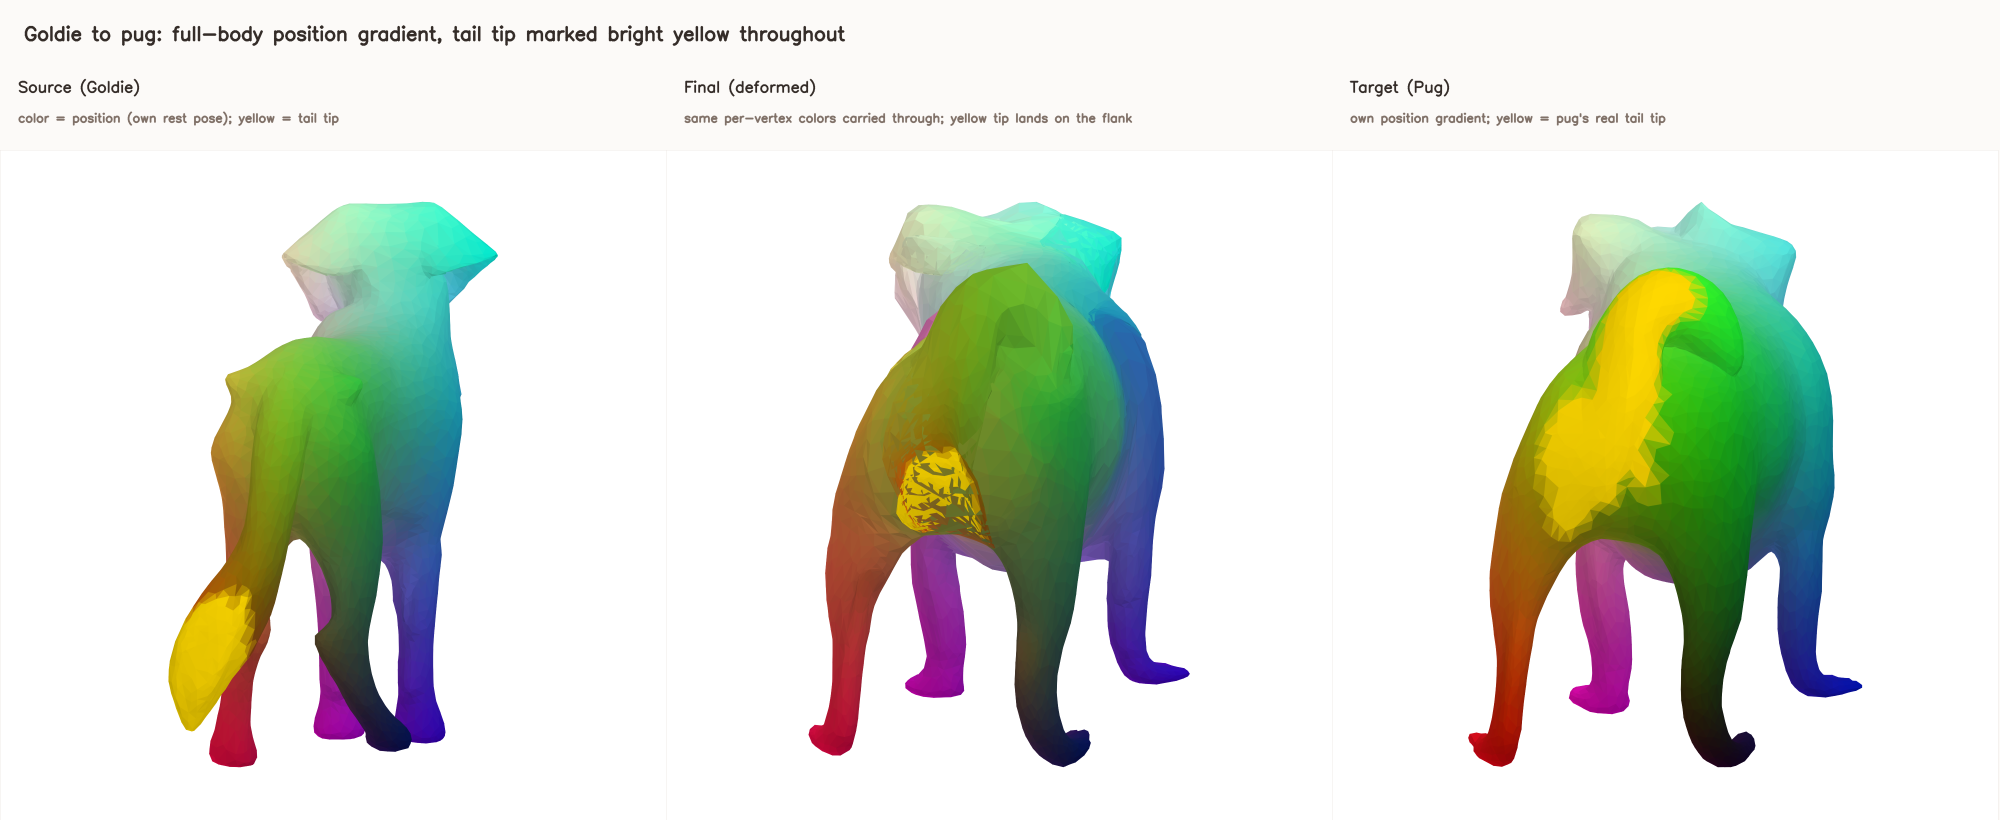
\includegraphics[width=0.98\textwidth]{figures/goldie_pug_tail_points.png}
\caption{Goldie $\rightarrow$ Pug tail-tip tracking. The source tail-tip vertices land on the
flank/hip rather than the target tail tip.}
\label{fig:goldie-pug-tail}
\end{figure}

\subsection{PartField bucket instability}

PartField buckets are unsupervised. They are useful precisely because they avoid manual labels, but
they are not guaranteed to be consistent across large shape gaps. A bucket that represents a leg on
one mesh can include body or neck points on another mesh. When this happens, the local Chamfer term
can guide the optimizer in the wrong direction.

\begin{figure}[H]
\centering
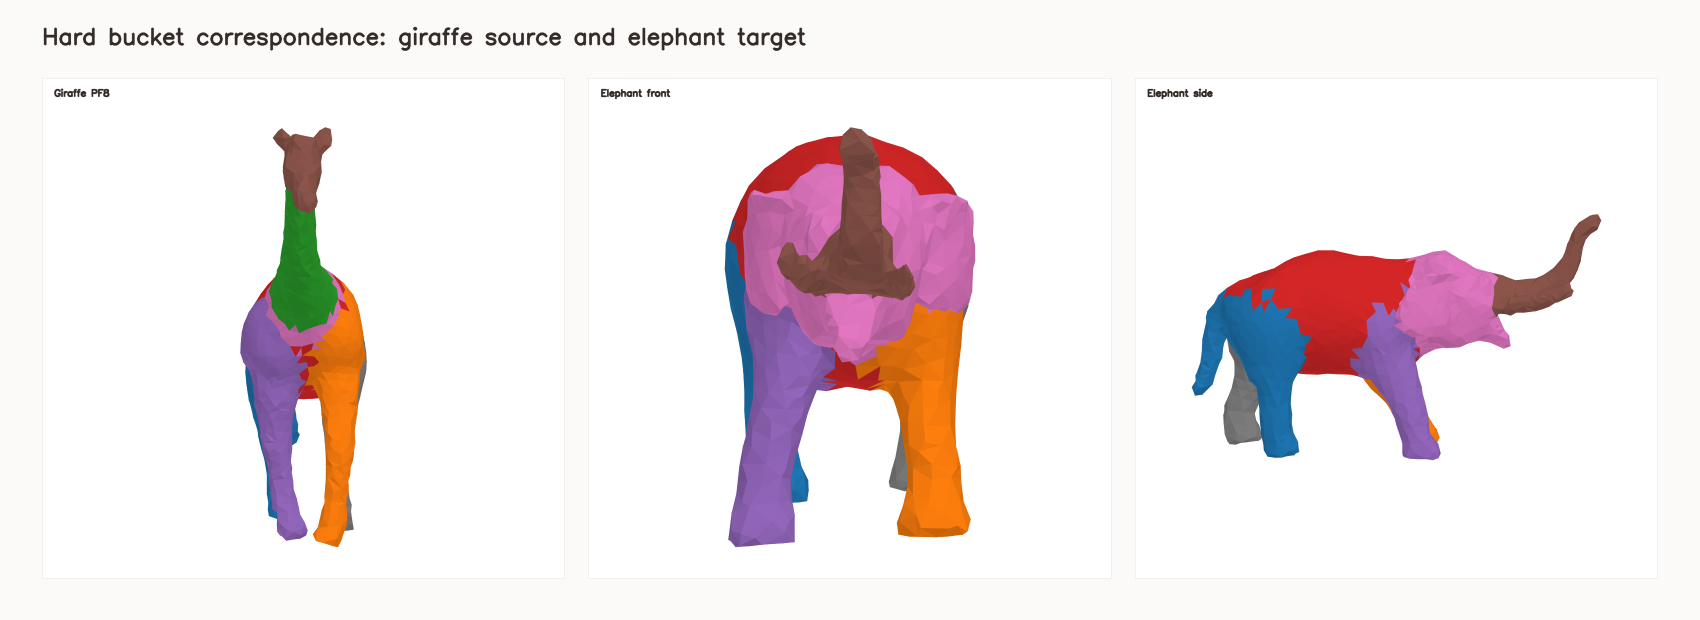
\includegraphics[width=0.86\textwidth]{figures/failure_worst_buckets.png}
\caption{Poor bucket correspondence in a difficult giraffe-to-elephant pair.}
\label{fig:failure-buckets}
\end{figure}

\begin{figure}[H]
\centering
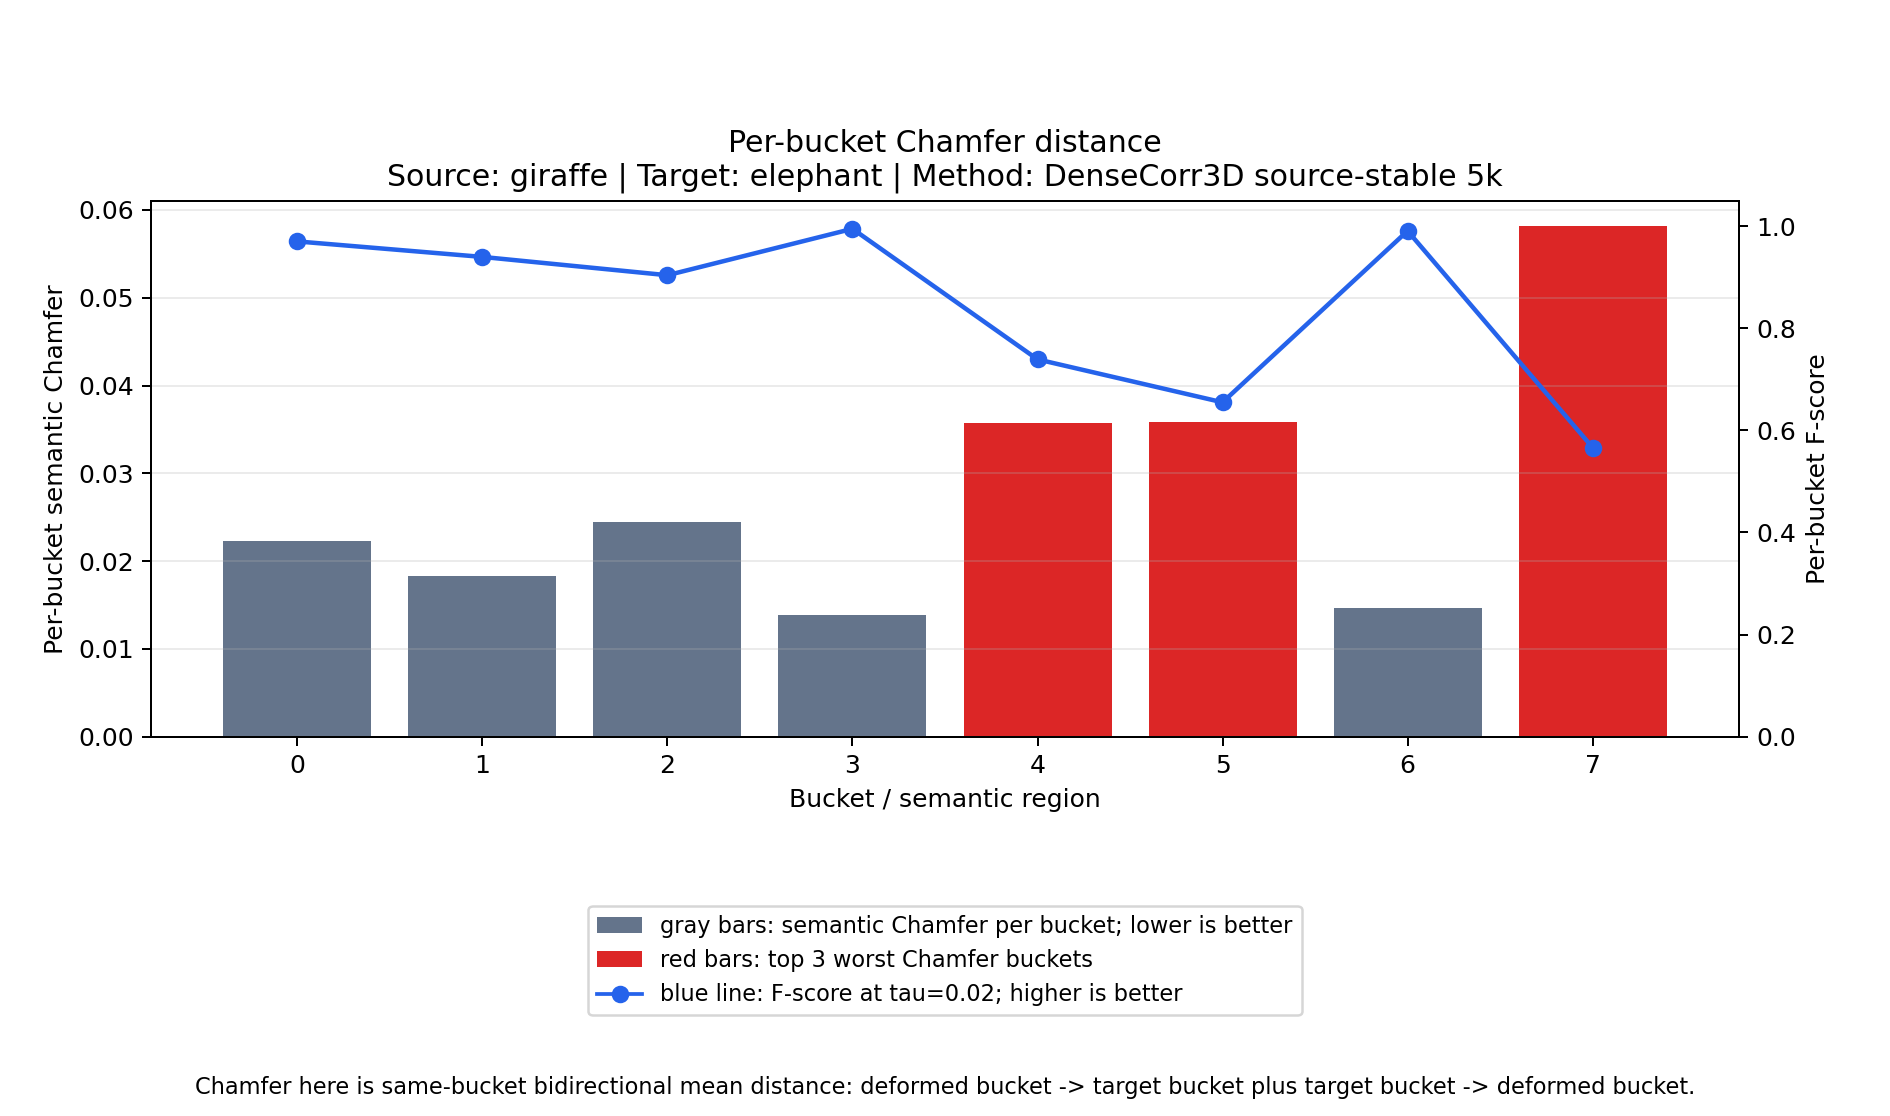
\includegraphics[width=0.70\textwidth]{figures/failure_bucket_chamfer.png}
\caption{Bucket-level Chamfer reveals which local regions dominate the error.}
\label{fig:failure-chamfer}
\end{figure}

\subsection{Orientation and pose}

Many failures are preprocessing failures, not deep failures of the deformation objective. If the
source faces forward and the target is rotated, or a category such as zucchini or egg has
inconsistent stem orientation, nearest-neighbor and PartField matching can be wrong from the start.

\begin{figure}[H]
\centering
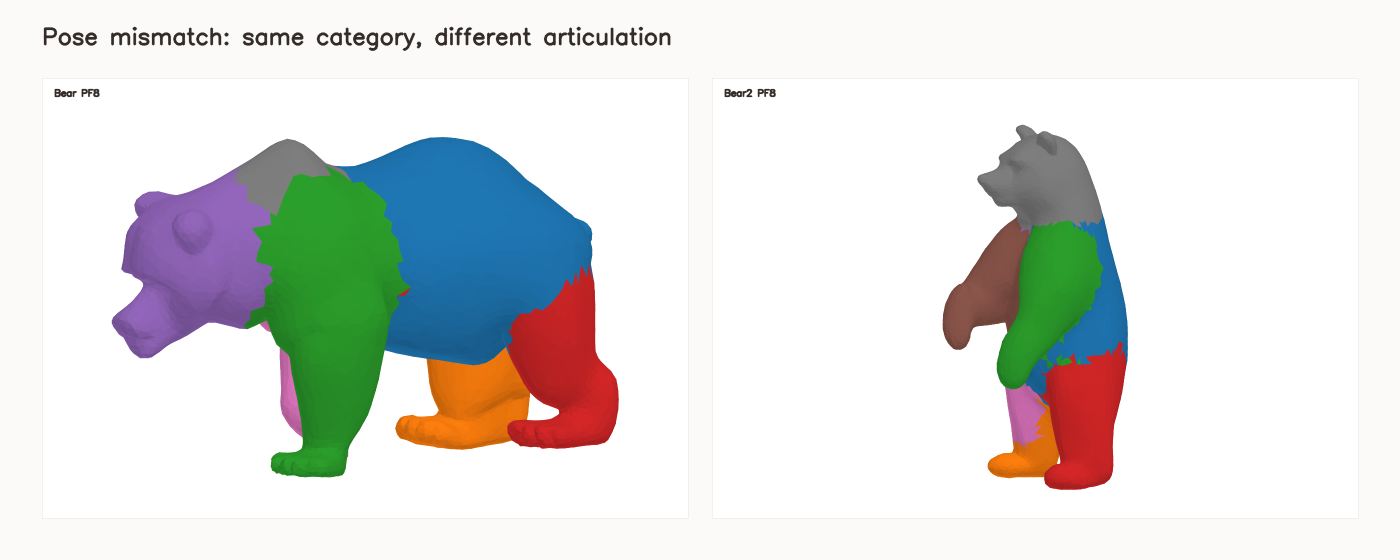
\includegraphics[width=0.80\textwidth]{figures/partfield_bear_pose_mismatch.png}
\caption{Pose mismatch can make local buckets disagree.}
\label{fig:pose-mismatch}
\end{figure}

\begin{figure}[H]
\begin{minipage}{0.45\textwidth}
\centering
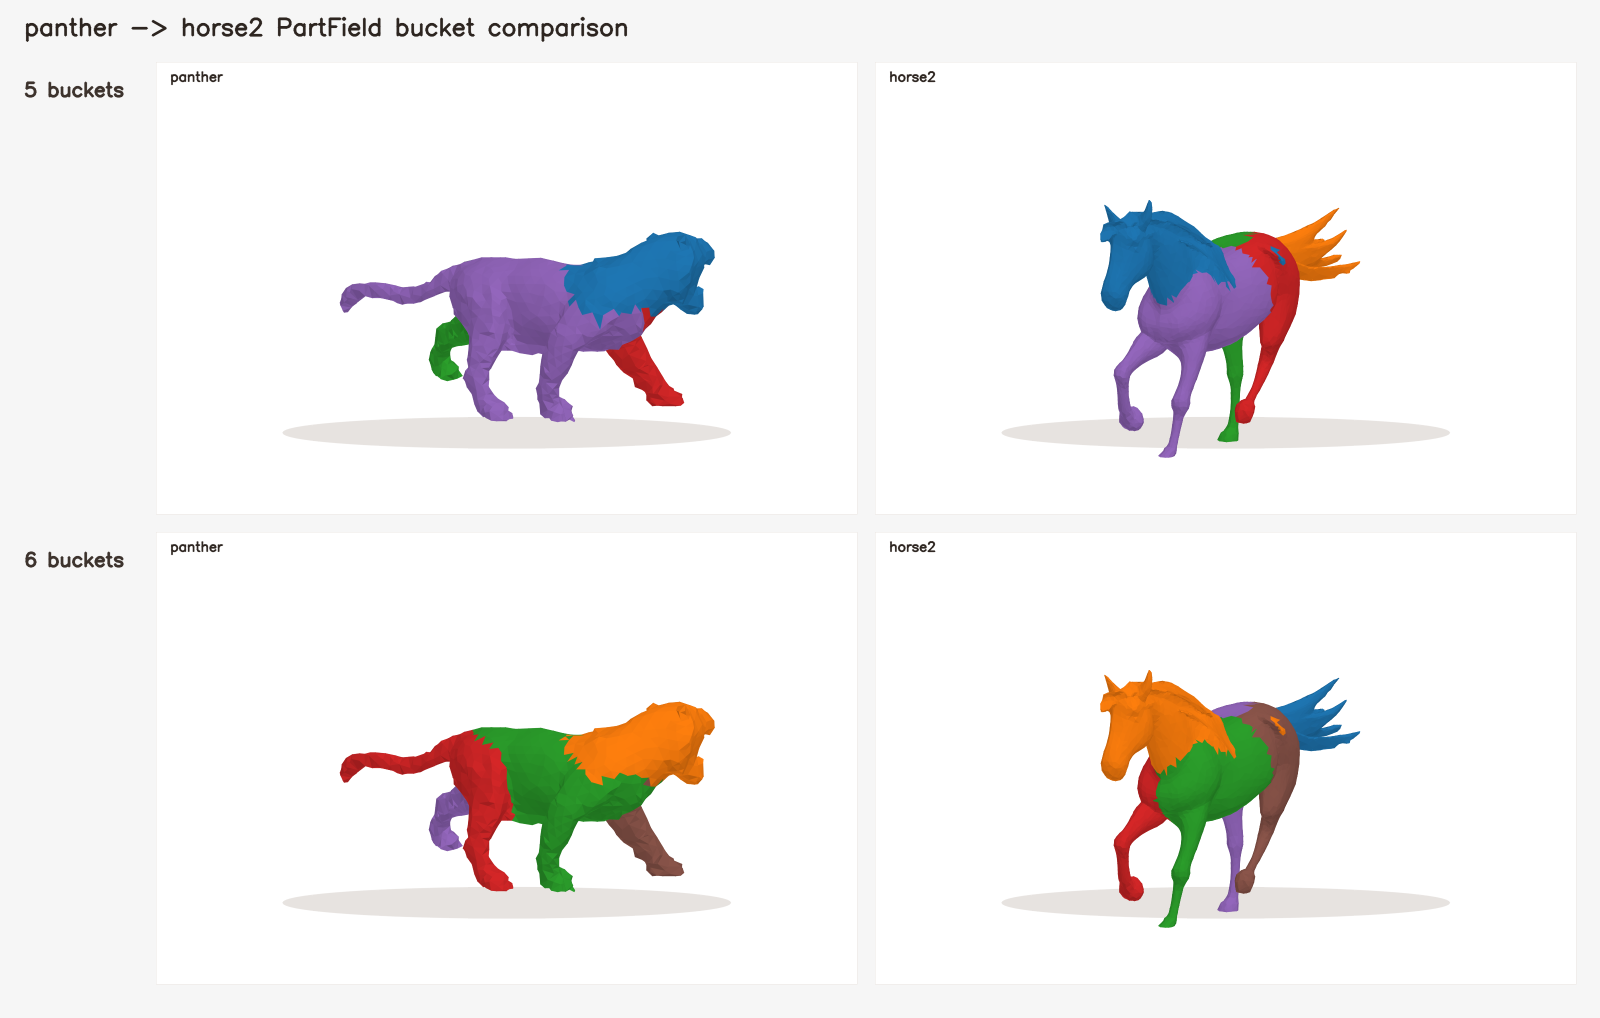
\includegraphics[width=0.96\linewidth]{figures/partfield_orientation_unaligned.png}
\caption{Unaligned orientation can make PartField buckets appear inconsistent.}
\label{fig:orientation-unaligned}
\end{minipage}
\hfill
\begin{minipage}{0.45\textwidth}
\centering
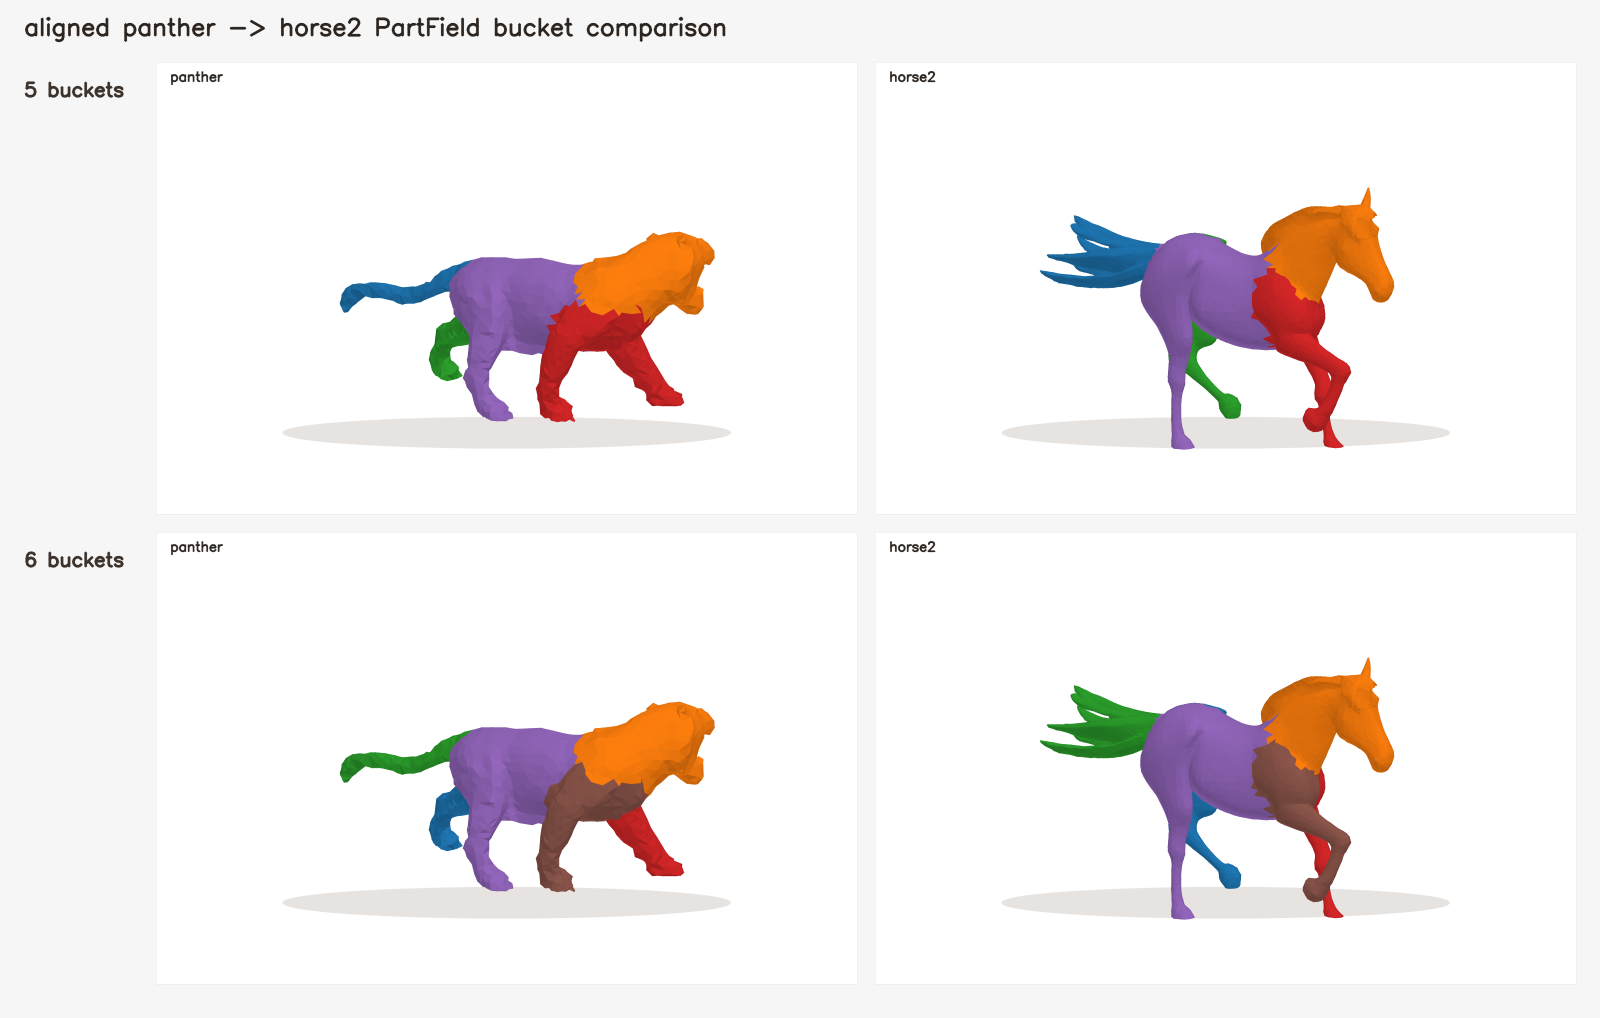
\includegraphics[width=0.96\linewidth]{figures/partfield_orientation_aligned.png}
\caption{After alignment, the same category often produces more interpretable buckets.}
\label{fig:orientation-aligned}
\end{minipage}
\end{figure}

\subsection{Metric sensitivity}

Metrics measure different properties. Chamfer may be low even when a small part is semantically
wrong. AUC can be strong while Err remains high if most points are good but some regions fail
badly. \Fscore{} at $0.02$ is strict and visually meaningful in unit-box coordinates, but sensitive
to small sampling and normalization choices. The most useful diagnostic pattern is disagreement
between the mean and the tail: if Chamfer is low but $p95$ is high, the result probably has a
localized severe failure; if AUC is high but Err is high, many points are correct but some are far
away along the target surface; if global \Fscore{} is strong but semantic \Fscore{} is weaker, the
mesh fits the target surface but the local regions are not matching cleanly.

\section{Discussion}

The strongest result of the project is that local part supervision changes the behavior of mesh
deformation in the intended direction, and that this holds up in the graph-geodesic comparison
against DenseMatcher's own predictions: on identical directed pairs, with the same scorer applied
to both methods, the pipeline wins $21$ of $23$ DenseCorr3D categories under the range-averaged,
zero-best-PF protocol.
The optimizer no longer sees the target as only an unordered surface. It sees a weak structural map
between source and target. A stricter clean-preparation subset gives the more conservative
cross-check: on $12$ categories without assisted preparation, it still beats DenseMatcher on $10$
of $12$ with zero best-PF selection. This supports the same
interpretation from the other side: the method benefits from a shared canonical orientation, as the
PartField examples in Figures~\ref{fig:orientation-unaligned}--\ref{fig:orientation-aligned} make
visible, but the main DenseMatcher improvement is not carried only by categories that received
extra pose help.

The second important result is that the method is diagnostically useful, in both directions. When
it fails, the failure traces to a concrete cause: orientation, bucket instability, topology
mismatch, or a category with no real part structure (Section~\ref{sec:root-cause}).

At the same time, the method is not a complete solution to dense 3D correspondence, and the
assisted-preparation subset remains a caveat that should be separated from the clean subset.
Its deeper, structural limitations -- what bounds it, and what would need to change to raise that
bound -- are addressed directly in Section~\ref{sec:limitations}. The right conclusion: PartField local 
guidance is a strong, audited practical prior for mesh
deformation, especially when the source and target share visible, non-rigid part structure, and its
limits are as well characterized as its strengths.

\section{Limitations}
\label{sec:limitations}

\textbf{The deformation is only ever as good as the segmentation that guides it.} PartField buckets
are an unsupervised proxy for correspondence, not correspondence itself: the local Chamfer term
only ever knows that ``source bucket $k$ should move toward target bucket $k$,'' and if that
assignment is wrong or unstable -- as Section~\ref{sec:root-cause} and Section~\ref{sec:failure-modes}
document in detail -- no amount of optimization, regularization, or curriculum tuning can recover
the correct correspondence from it. This is the ceiling on the whole approach, and it is a
structural one, not a tuning problem.

The clearest evidence for that ceiling is what happens when the bottleneck is removed. As a
diagnostic, this pipeline was also run on TOSCA~\cite{tosca} pairs spanning five categories (cat,
dog, gorilla, horse, wolf) using each pair's real, dense, ground-truth vertex correspondence as the
only guidance signal, in place of PartField buckets entirely (the same Jacobian deformation
machinery, with the local-bucket Chamfer term replaced by a direct per-vertex correspondence loss).
Figure~\ref{fig:tosca-ceiling} shows three of these pairs -- dog, gorilla, and horse -- each with a
large pose change: in every case the deformed source is visually almost indistinguishable from the
target. Scored with the same graph-geodesic evaluator used throughout this report, and averaged over every
one of the $23$ completed TOSCA dense-correspondence runs in the project (not a selected subset),
these runs reach mean AUC $0.950$ and mean Err $1.40$ (best pair: wolf0$\to$wolf2, AUC
$1.000$/Err $0.001$; weakest: cat0$\to$cat2, AUC $0.786$/Err $5.72$), clearly above this pipeline's
own headline PartField-guided numbers (AUC $0.824$/Err $4.77$ across all $23$ DenseCorr3D
categories, Table~\ref{tab:densematcher-headline}). This is not a claim that dense correspondence
is free -- TOSCA pairs come with correspondence already solved, which is exactly the hard problem
PartField is standing in for -- but it suggests that an important remaining gap comes from the
quality of the correspondence signal feeding the deformation, not only from the deformation
representation itself.

\begin{figure}[H]
\centering
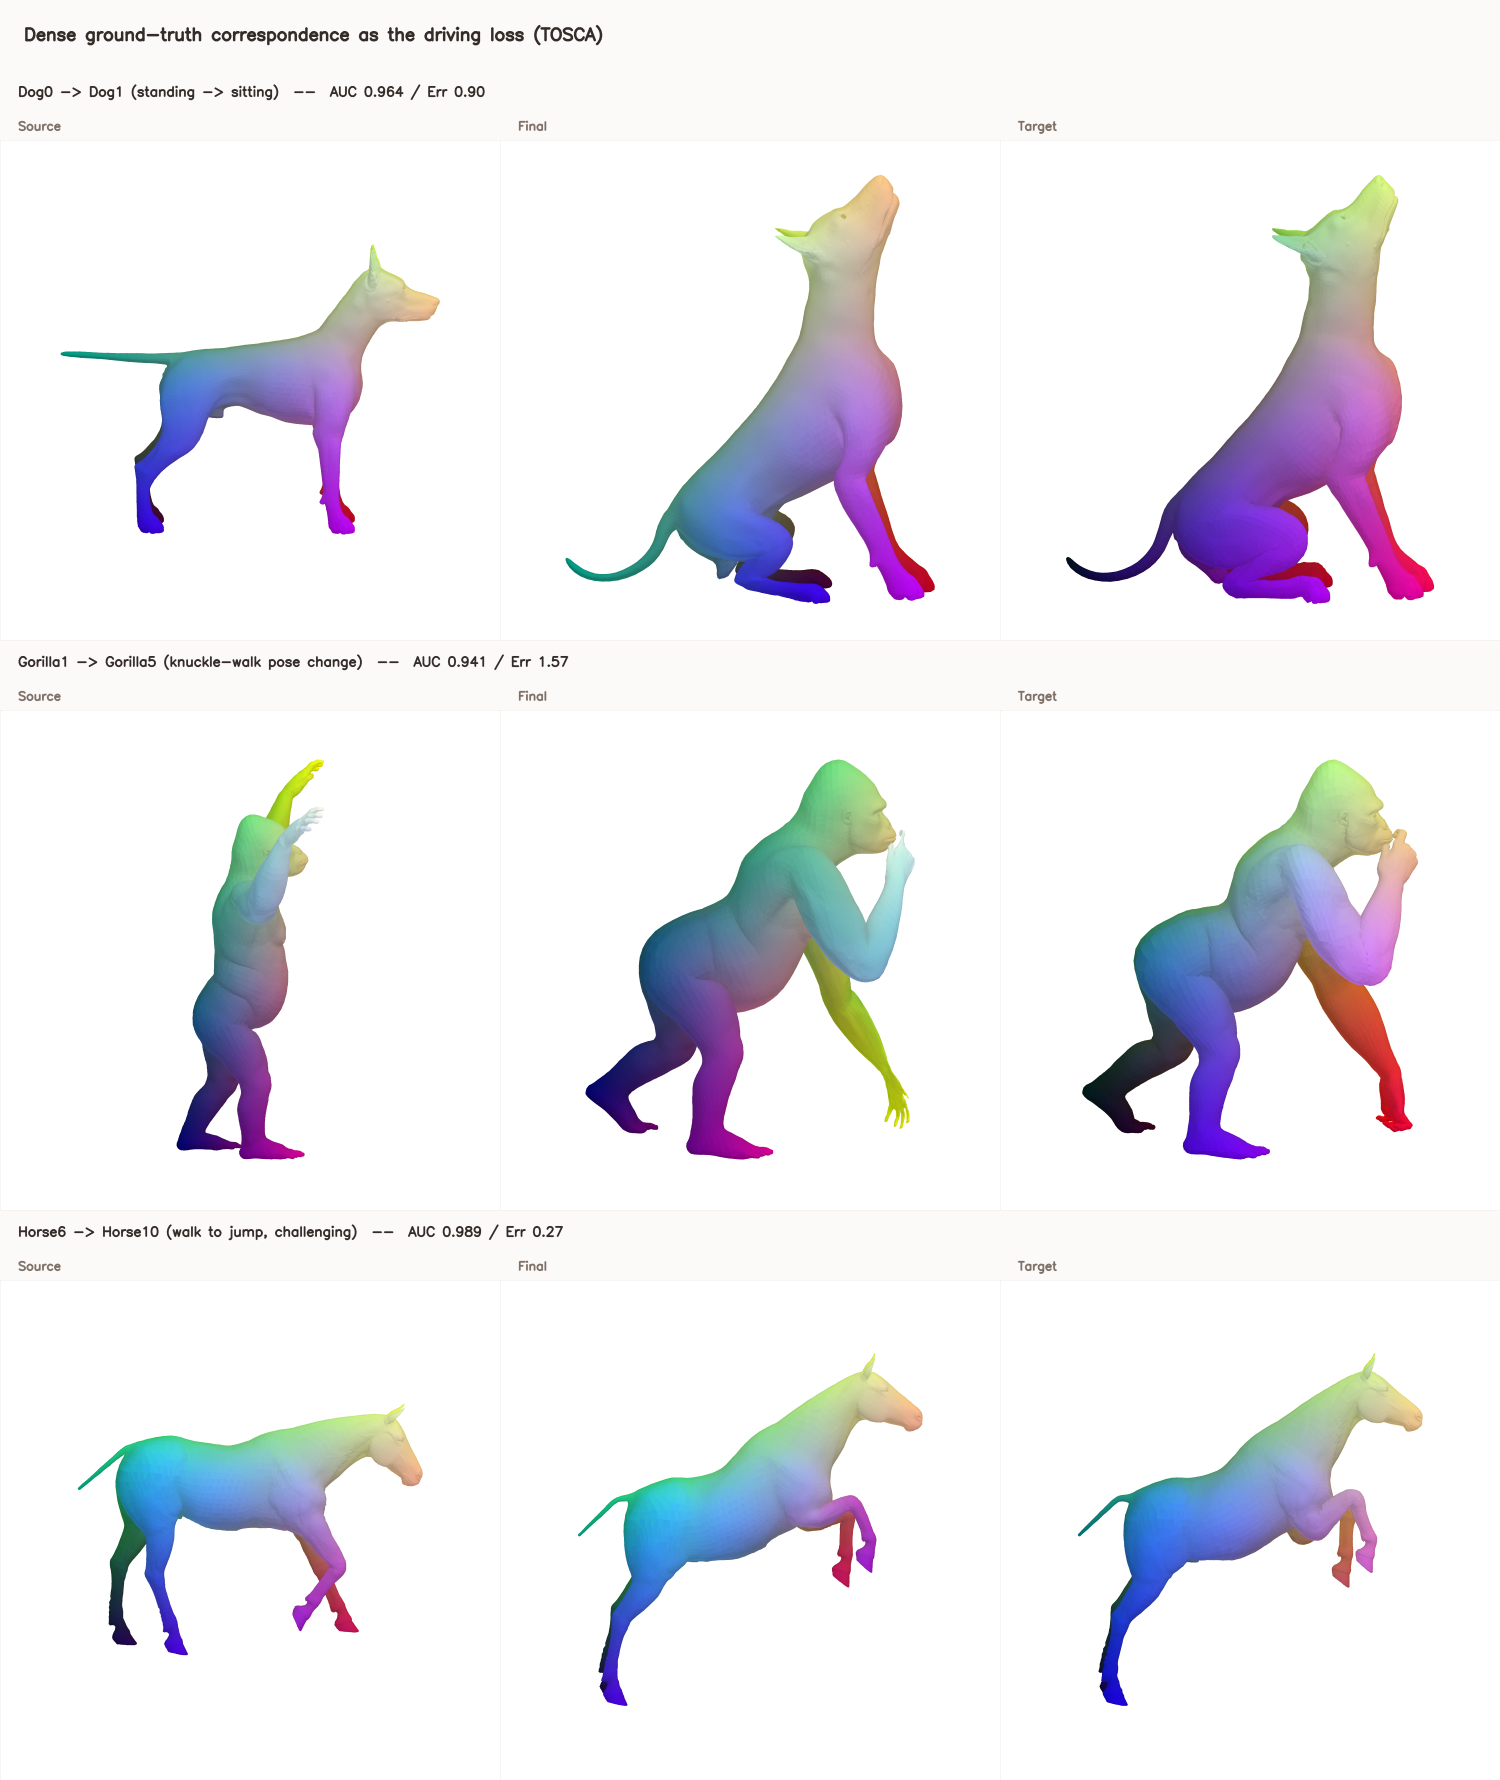
\includegraphics[width=0.95\textwidth]{figures/tosca_dense_corr_ceiling.png}
\caption{TOSCA dense-correspondence ceiling test: with ground-truth guidance, the deformation
representation is usually not the bottleneck.}
\label{fig:tosca-ceiling}
\end{figure}

\begin{table}[H]
\centering
\scriptsize
\begin{tabularx}{\textwidth}{lX}
\toprule
Category & Completed TOSCA dense-correspondence-guided runs \\
\midrule
cat & cat0$\to$cat1, cat0$\to$cat2, cat1$\to$cat4, cat2$\to$cat5, cat3$\to$cat9 \\
dog & dog0$\to$dog1, dog0$\to$dog2, dog1$\to$dog3, dog2$\to$dog5, dog6$\to$dog8 \\
horse & horse0$\to$horse5, horse0$\to$horse6, horse5$\to$horse7, horse6$\to$horse10, horse14$\to$horse15 \\
wolf & wolf0$\to$wolf1, wolf0$\to$wolf2, wolf1$\to$wolf2 \\
gorilla & gorilla1$\to$gorilla5, gorilla1$\to$gorilla8, gorilla1$\to$gorilla14, gorilla5$\to$gorilla8, gorilla8$\to$gorilla14 \\
\bottomrule
\end{tabularx}
\caption{All 23 completed TOSCA dense-correspondence-guided runs used for the aggregate ceiling
diagnostic. Figure~\ref{fig:tosca-ceiling} renders three representative examples from this list.}
\label{tab:tosca-runs}
\end{table}

\textbf{Fixed topology: no new parts can be created.} The deformation moves an existing mesh; it
cannot introduce a new limb, horn, or disconnected component that the source does not already have
some surface area to repurpose. When the target genuinely needs one -- an elephant's trunk, a
giraffe's ossicones, a missing limb -- the pipeline can only approximate it by stealing area from a
neighboring source part (Section~\ref{sec:failure-modes}), which is part of why the SAM3D vehicle
results in particular do not close the gap: rigid, sharply-creased geometry has essentially no
slack part to repurpose this way.

\textbf{Vertices are moved, never deleted.} The Jacobian-field parameterization
(Section~\ref{sec:deformation-repr}) changes vertex positions; it has no mechanism to remove a
vertex or a face. If the target is smaller or simpler than the source in some region, that source
geometry cannot disappear -- it can only be compressed, flattened, or folded into a thinner sliver,
which is a recurring source of the self-intersection and surface-quality problems documented in
Section~\ref{sec:surface-quality}.

\section{Future Work}
\label{sec:future-work}

Several extensions follow naturally from the experiments.

\begin{enumerate}
  \item \textbf{Closing the segmentation ceiling with real dense correspondence.}
  Section~\ref{sec:limitations} suggests that replacing PartField buckets with real dense
  correspondence substantially raises the achievable ceiling (23 TOSCA pairs: mean AUC
  $0.950$ vs.\ this pipeline's own $0.824$ headline). Learning or acquiring a real dense
  correspondence predictor, rather than relying on unsupervised segmentation matching, is the
  single change most likely to improve results beyond what better buckets or more regularization
  can achieve.
  \item \textbf{Learned bucket matching.} A smaller step in the same direction: instead of assuming
  bucket $k$ matches bucket $k$, learn a soft transport matrix between source and target buckets.
  \item \textbf{Learned bucket-count selection.} The LLM-based bucket selector
  (Section~\ref{sec:system-overview}) was built for pipeline completeness rather than as a benchmarked
  component; replacing its prompt-based reasoning with a selector trained on which $K$ actually
  performs best for a given pair is a natural next step.
  \item \textbf{Topology-aware deformation for rigid domains.} The vehicle results in
  Section~\ref{sec:surface-quality} suggest that fixed-topology deformation is a worse fit for rigid,
  sharply-creased bodies than for articulated ones; remeshing, implicit surfaces, or panel-aware
  segmentation are more promising directions there than further loss-weight tuning.
  \item \textbf{Category-level evaluation with a fixed protocol.} Convert the strongest selected-pair
  results into a benchmark protocol with predetermined PF levels and no per-pair model selection,
  matching the zero-selection standard already applied to the DenseMatcher comparison.
  \item \textbf{Better semantic diagnostics.} Report bucket transport entropy, per-part failure
  curves, and confidence maps so bad correspondences can be identified automatically rather than by
  manual inspection.
\end{enumerate}

\section{Conclusion}

This project built and evaluated a semantic-guided part-aware mesh deformation pipeline, after 
redirecting away
from an earlier, heavier image-semantic approach built on MeshUp (Appendix~\ref{app:meshup}).
Starting from a source and target mesh, the method uses PartField buckets to turn global shape
matching into a more structured problem: the whole surface should match, but corresponding local
parts should match as well. Evaluated against DenseMatcher's own predicted correspondences on
identical directed pairs, using the same graph-geodesic evaluator applied to both methods, the method
 wins $21$ of $23$ categories with
predeclared category-specific PF ranges and no best-PF picking within those ranges. It gives clean
surface geometry on articulated self-created
SAM3D pairs, exposes weaknesses and traces its failure cases down to specific, identifiable 
causes -- orientation, unstable
buckets, topology mismatch, or evaluator sensitivity. The main contribution is therefore a practical, 
interpretable, and audited
deformation pipeline: simple enough to analyze, structured enough to avoid many of the semantic
mistakes made by pure Chamfer optimization, and evaluated with the same scrutiny applied to its
strongest results as to its weaknesses.

\clearpage
\appendix

\section{Earlier Work: Adding Semantic Awareness to MeshUp}
\label{app:meshup}

Before the project became a direct mesh-to-mesh deformation pipeline, the initial direction was to
make MeshUp more semantically aware. MeshUp is a multi-target mesh deformation method that uses
score distillation and differentiable rendering to guide a source mesh toward image-level target
concepts~\cite{meshup}. This is powerful because it can use image priors, but it is not inherently a
dense 3D correspondence method. The optimizer sees rendered images and global shape regularization.
It does not automatically know that the tip of one tail should follow the tip of another tail, or
that a leg should correspond to a leg across different animals.

The motivation for the first set of experiments was therefore simple: add semantic feature signals
to the MeshUp loop. The project explored DINO-style visual features, DINO PCA visualizations,
semantic vertex correspondences, and a preliminary RAE-DiT teacher idea. In the image-feature
branch, the mesh was rendered from several views, the rendered images were passed through
DINOv2-style feature encoders~\cite{dinov2}, and the resulting feature maps were used as semantic
guidance. In the diffusion branch, the original MeshUp-style score-distillation setup was still
present, using the same broad idea as DreamFusion: optimize a 3D object through gradients obtained
from a 2D generative prior~\cite{dreamfusion}. The tracked configuration used an XL DeepFloyd IF
stage, a large cascaded text-to-image diffusion model; the public model card lists the Stage-I XL
model at about $4.3$ billion parameters~\cite{deepfloydif}.

This direction was scientifically reasonable, but it had a practical problem: the semantic signal
remained indirect. DINO features are extracted from rendered views, not from stable 3D surface
points. A feature that appears reliable in one camera can become ambiguous under occlusion, pose
change, lighting, or a different silhouette. Similarly, diffusion gradients can encourage a
plausible rendered image without producing a clean point-to-point or part-to-part surface
correspondence. In other words, the old pipeline was trying to obtain 3D semantic deformation from
2D semantic supervision.

\begin{table}[H]
\centering
\scriptsize
\begin{tabularx}{\textwidth}{>{\raggedright\arraybackslash}p{0.20\textwidth}r>{\raggedright\arraybackslash}p{0.16\textwidth}rrr>{\raggedright\arraybackslash}X}
\toprule
Run & Epochs & Main guidance & Time & Peak RAM & FID $\downarrow$ & Interpretation \\
\midrule
A1 baseline dev & 2500 & SDS, no DINO & 24:10 & 12.5 GiB & 605.19 &
Reference dev run. \\
A1 DINO dev & 2500 & SDS + DINO & 24:49 & 12.1 GiB & 592.20 &
DINO improved FID by 12.99 points, about 2.15\%, but the gain was small. \\
A1 baseline non-dev & 2500 & SDS, no DINO & 28:00 & 14.9 GiB & 494.86 &
Stronger baseline run without DINO. \\
A1 DINO non-dev & 6000 & SDS + DINO & 56:13 & 16.4 GiB & 503.35 &
Longer DINO run did not beat the shorter non-DINO baseline. \\
\bottomrule
\end{tabularx}
\caption{Early MeshUp semantic-guidance ablation. FID was useful as an image-level diagnostic, but
not a direct 3D correspondence metric. The DINO gain was small in the controlled dev comparison and
disappeared in the longer non-dev comparison.}
\label{tab:appendix-semantic-ablation}
\end{table}

The compute profile reinforced this conclusion. The tracked MeshUp configuration used
\texttt{batch\_size=8}, \texttt{accum\_iter=2}, and an XL diffusion model. At $2500$ epochs this
corresponds to roughly $80{,}000$ diffusion U-Net batch-item evaluations; at $6000$ epochs, roughly
$192{,}000$. The DINO side was also not free: with eight rendered views at approximately $512$
pixels, the feature extractor handled about $10{,}368$ patch tokens per mesh state before any
matching or loss computation. The old jobs were submitted with large memory envelopes, including
$40$\,GB for the ablations and a $64$\,GB DINO presentation script -- compare Section~\ref{sec:runtime}, where
the final PartField pipeline's representative runs measured under $1.8$\,GiB peak RAM.

\begin{table}[H]
\centering
\small
\begin{tabularx}{\textwidth}{>{\raggedright\arraybackslash}p{0.22\textwidth}XXX}
\toprule
Branch & Main signal & Evidence from the project & Outcome \\
\midrule
SDS + DINO MeshUp &
Rendered-image diffusion gradients plus rendered DINO features. &
Small dev FID gain; longer DINO run worse than shorter baseline; $40$--$64$ GB job envelopes;
tens of thousands of diffusion evaluations. &
Useful exploration, but too expensive and too indirect for the main report. \\
Semantic vertex correspondences &
PartField descriptors, bounding-box position, normals, and optional labels used to map source
vertices to target vertices. &
Dachshund $\rightarrow$ cat produced $3111/4712$ unique target vertices and $0.9291$ PartField
label agreement, but many vertices still collapsed to repeated targets. &
Good diagnostic signal, but direct semantic losses damaged geometry in difficult cases. \\
Semantic reindexing after topomatch &
Use clean geometry from topomatch, then reorder vertices according to the semantic map. &
Dog-pair label agreement ranged from about $0.70$ to $0.86$, with exact geometric recovery when the
operation was pure reindexing. &
Useful for correspondence analysis, but not a new deformation force and only exact for matching
topology. \\
Current PartField mesh-to-mesh deformation &
Global Chamfer, local bucket Chamfer, bucket balancing, and regularization directly in 3D. &
Representative final jobs ran in about $4.6$--$17.5$ minutes, with measured peak RAM below
$1.8$ GiB. &
Chosen direction: simpler, more interpretable, and evaluated with direct 3D metrics, now including
a same-evaluator comparison against a real correspondence method. \\
\bottomrule
\end{tabularx}
\caption{Why the project pivoted from image-semantic MeshUp guidance to direct mesh-to-mesh
deformation. The new pipeline does not give up on semantics; it moves semantic structure into
explicit 3D part supervision.}
\label{tab:appendix-pivot}
\end{table}

The final method still tries to deform semantically meaningful parts, but it does so through PartField
buckets, global and local Chamfer losses, bucket balancing, regularization, and 3D evaluation. This made the experiments easier
to interpret, and, ultimately, made it possible to run the much stronger same-evaluator comparison
against DenseMatcher in Section~\ref{sec:densematcher-fair} -- a comparison that would not have been
meaningful for a method whose main signal was 2D-rendered image similarity.

\section{Additional Qualitative Results}
\label{app:additional-qualitative}

\begin{figure}[H]
\centering
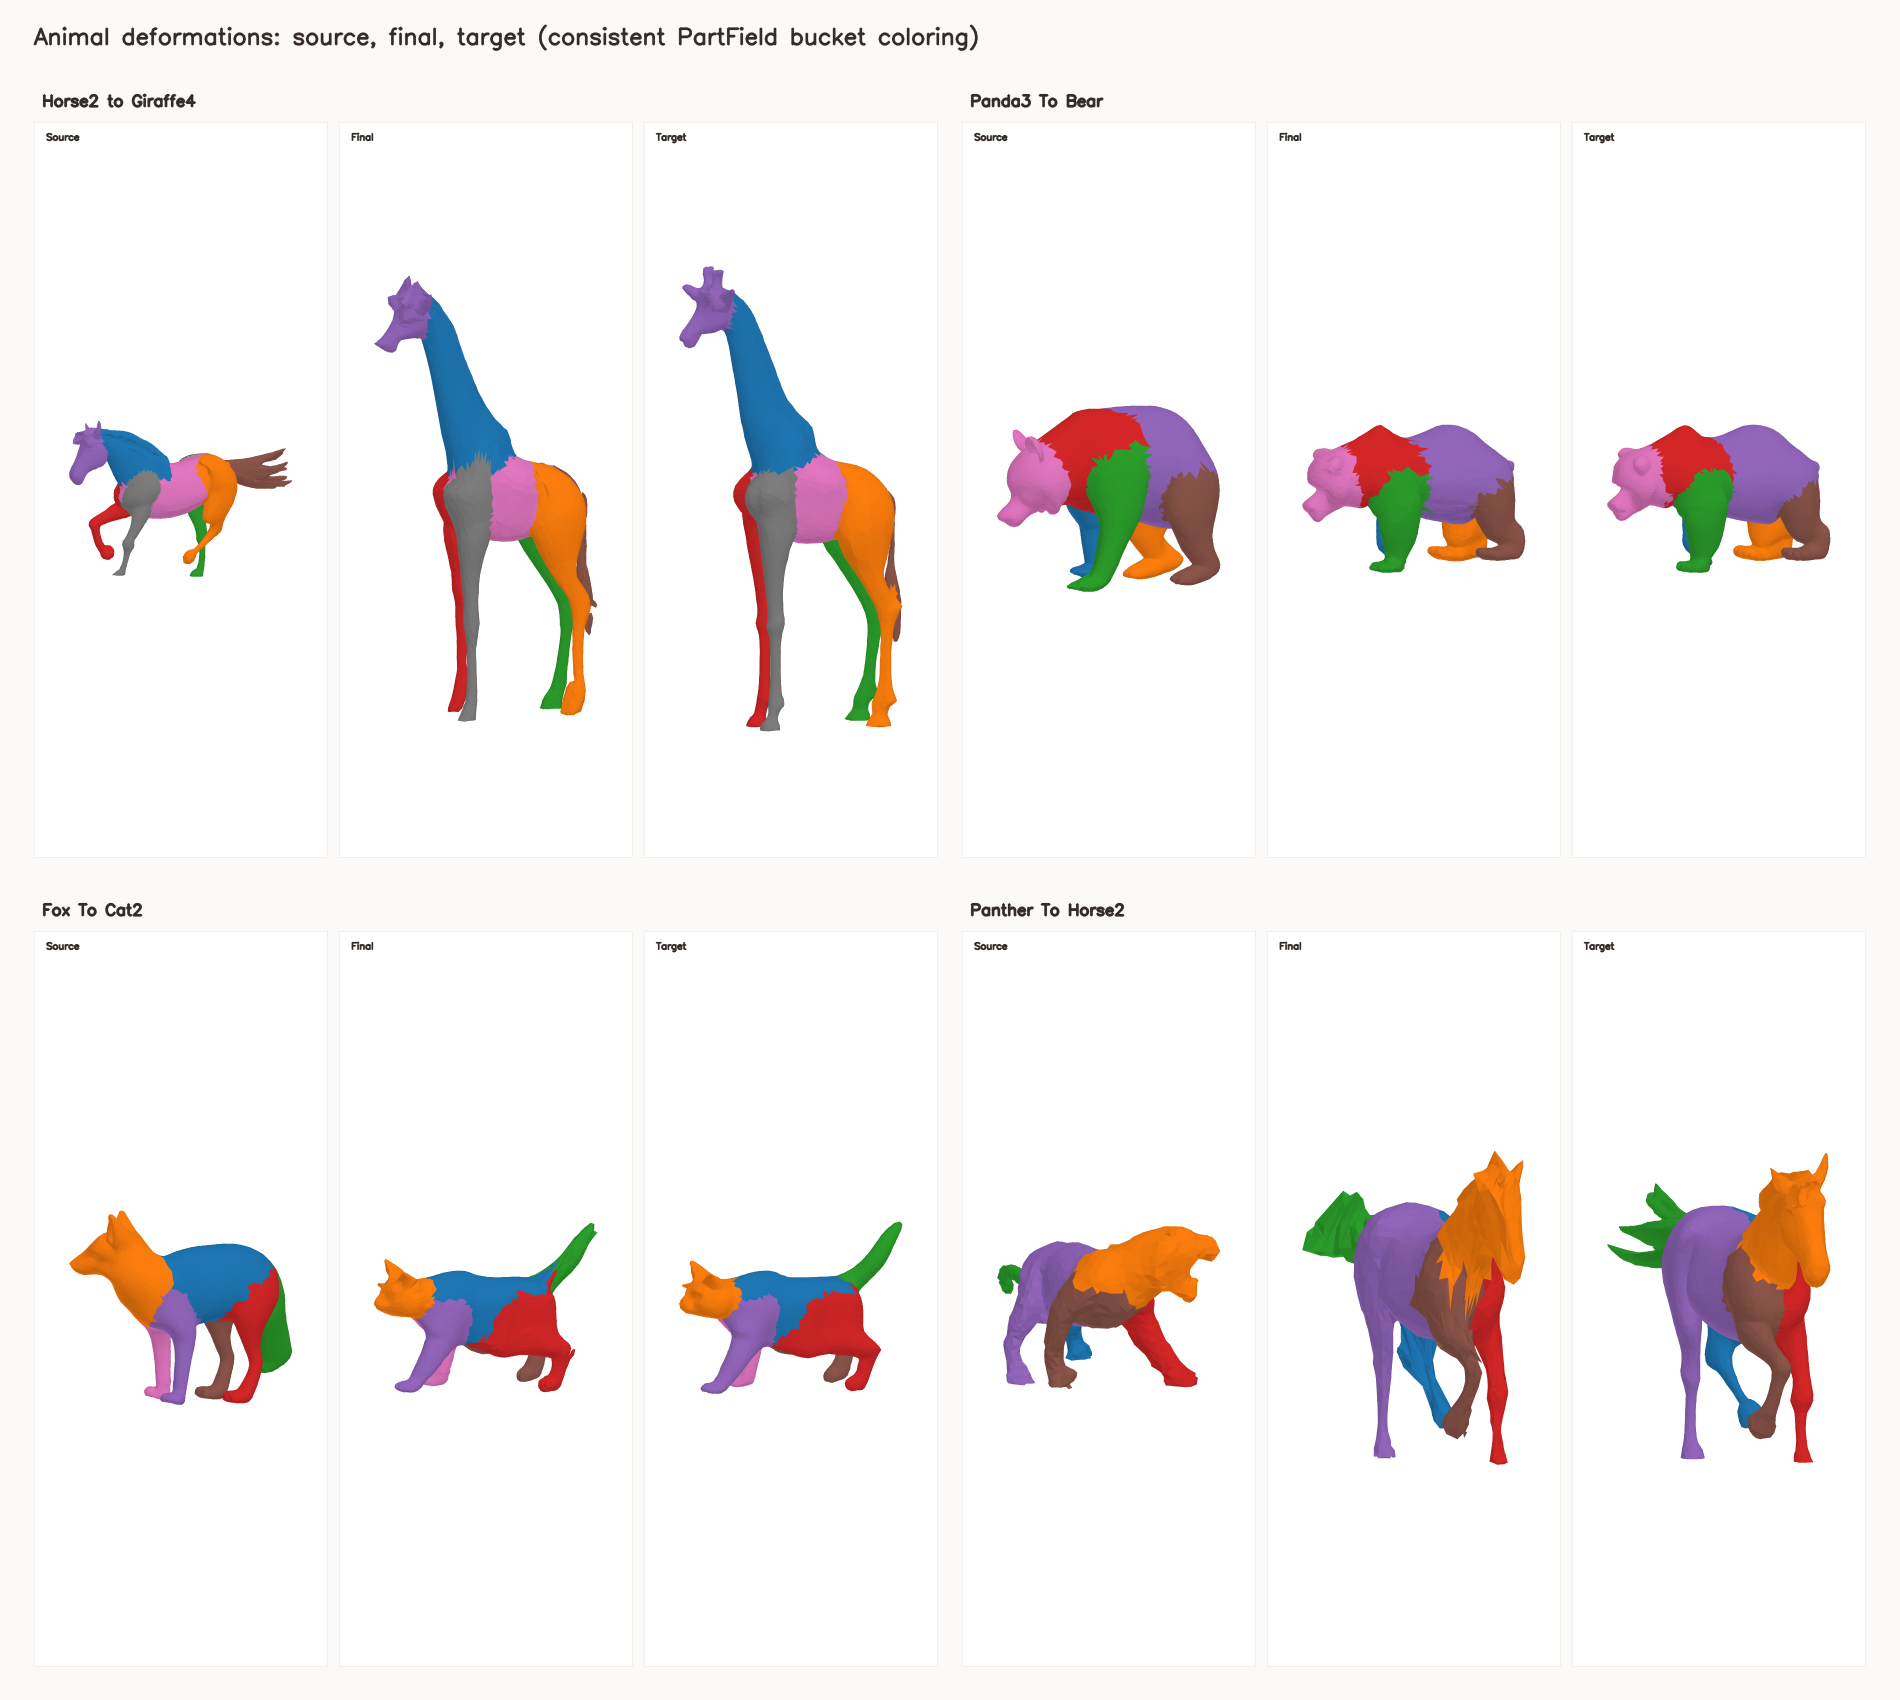
\includegraphics[width=0.94\textwidth]{figures/domain_animals_showcase.png}
\caption{Animal deformation showcase with consistent discrete PartField bucket coloring.}
\label{fig:domain-animals}
\end{figure}

Figure~\ref{fig:domain-animals} summarizes why animals are both compelling and difficult. The
method can stretch a horse toward a giraffe, a panda toward a bear, a fox toward a cat, or a
panther toward a horse while keeping local regions coherent. At the same time, animals contain
limbs, tails, necks, and heads whose correspondence depends on pose, which is why animal results
need both numerical evaluation and visual inspection.

\begin{figure}[H]
\centering
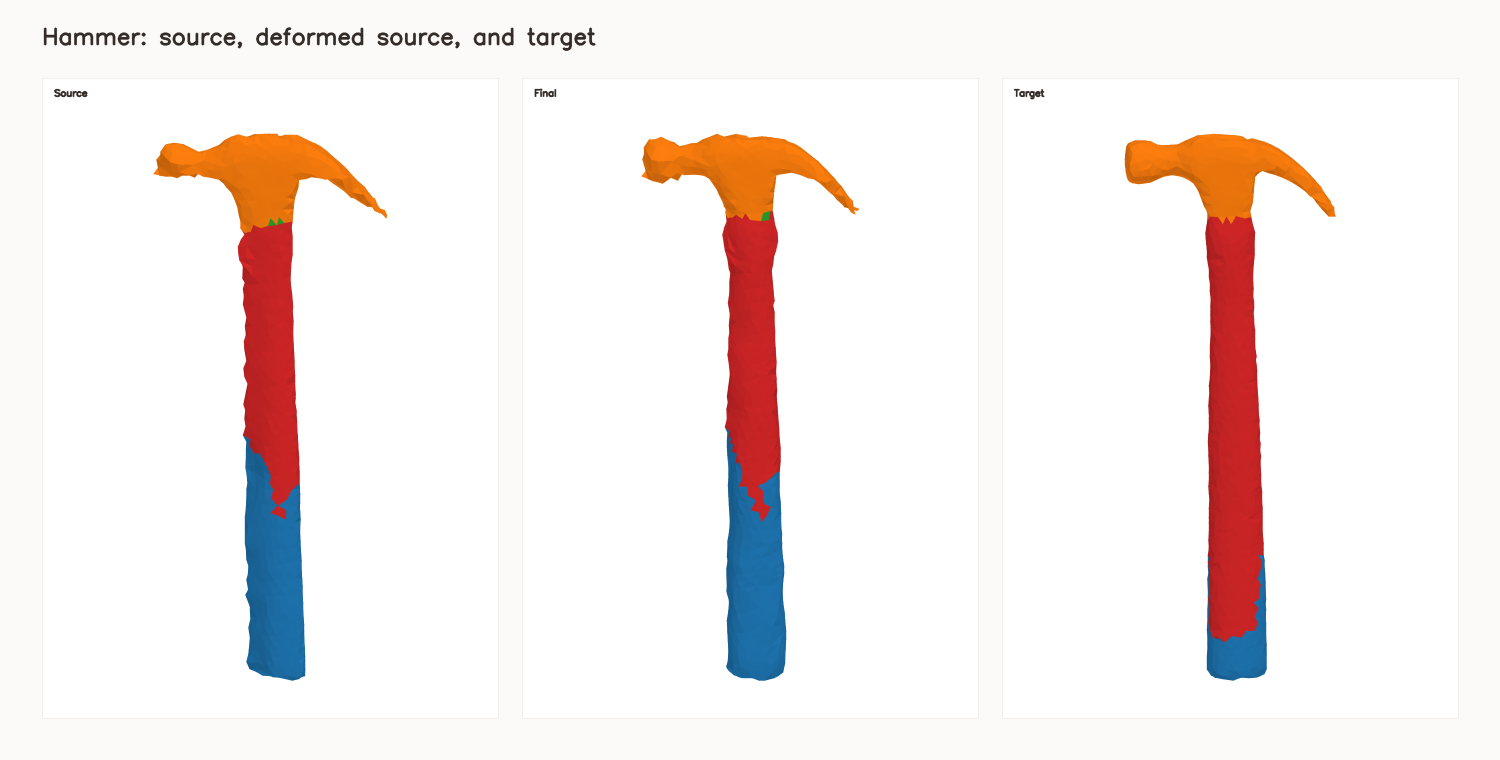
\includegraphics[width=0.82\textwidth]{figures/qual_hammer_result.png}
\caption{Hammer deformation: a stable handle/head structure gives PartField clear anchors.}
\label{fig:hammer}
\end{figure}

\begin{figure}[H]
\centering
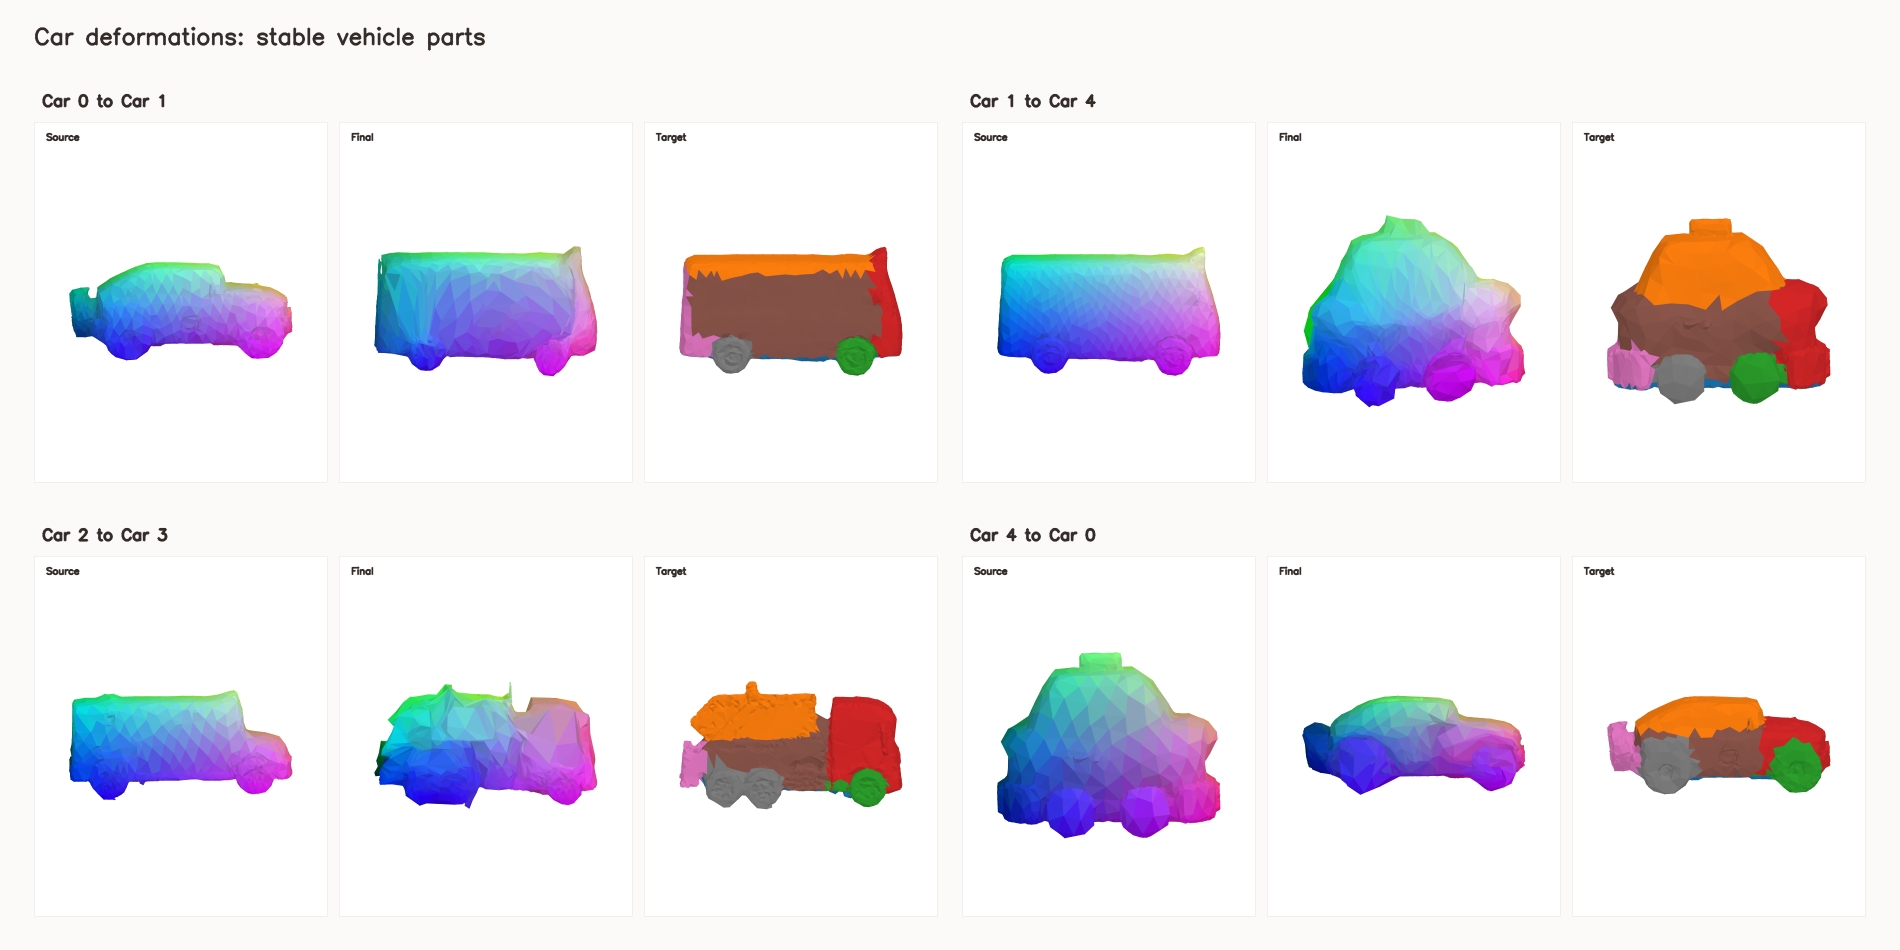
\includegraphics[width=0.90\textwidth]{figures/domain_cars_showcase.png}
\caption{Car deformation showcase on the DenseCorr3D benchmark category. Source and final panels
use inherited source-position coloring; target panels use PartField bucket coloring, so colors are
not direct cross-panel correspondence labels in this figure.}
\label{fig:domain-cars}
\end{figure}

\begin{figure}[H]
\centering
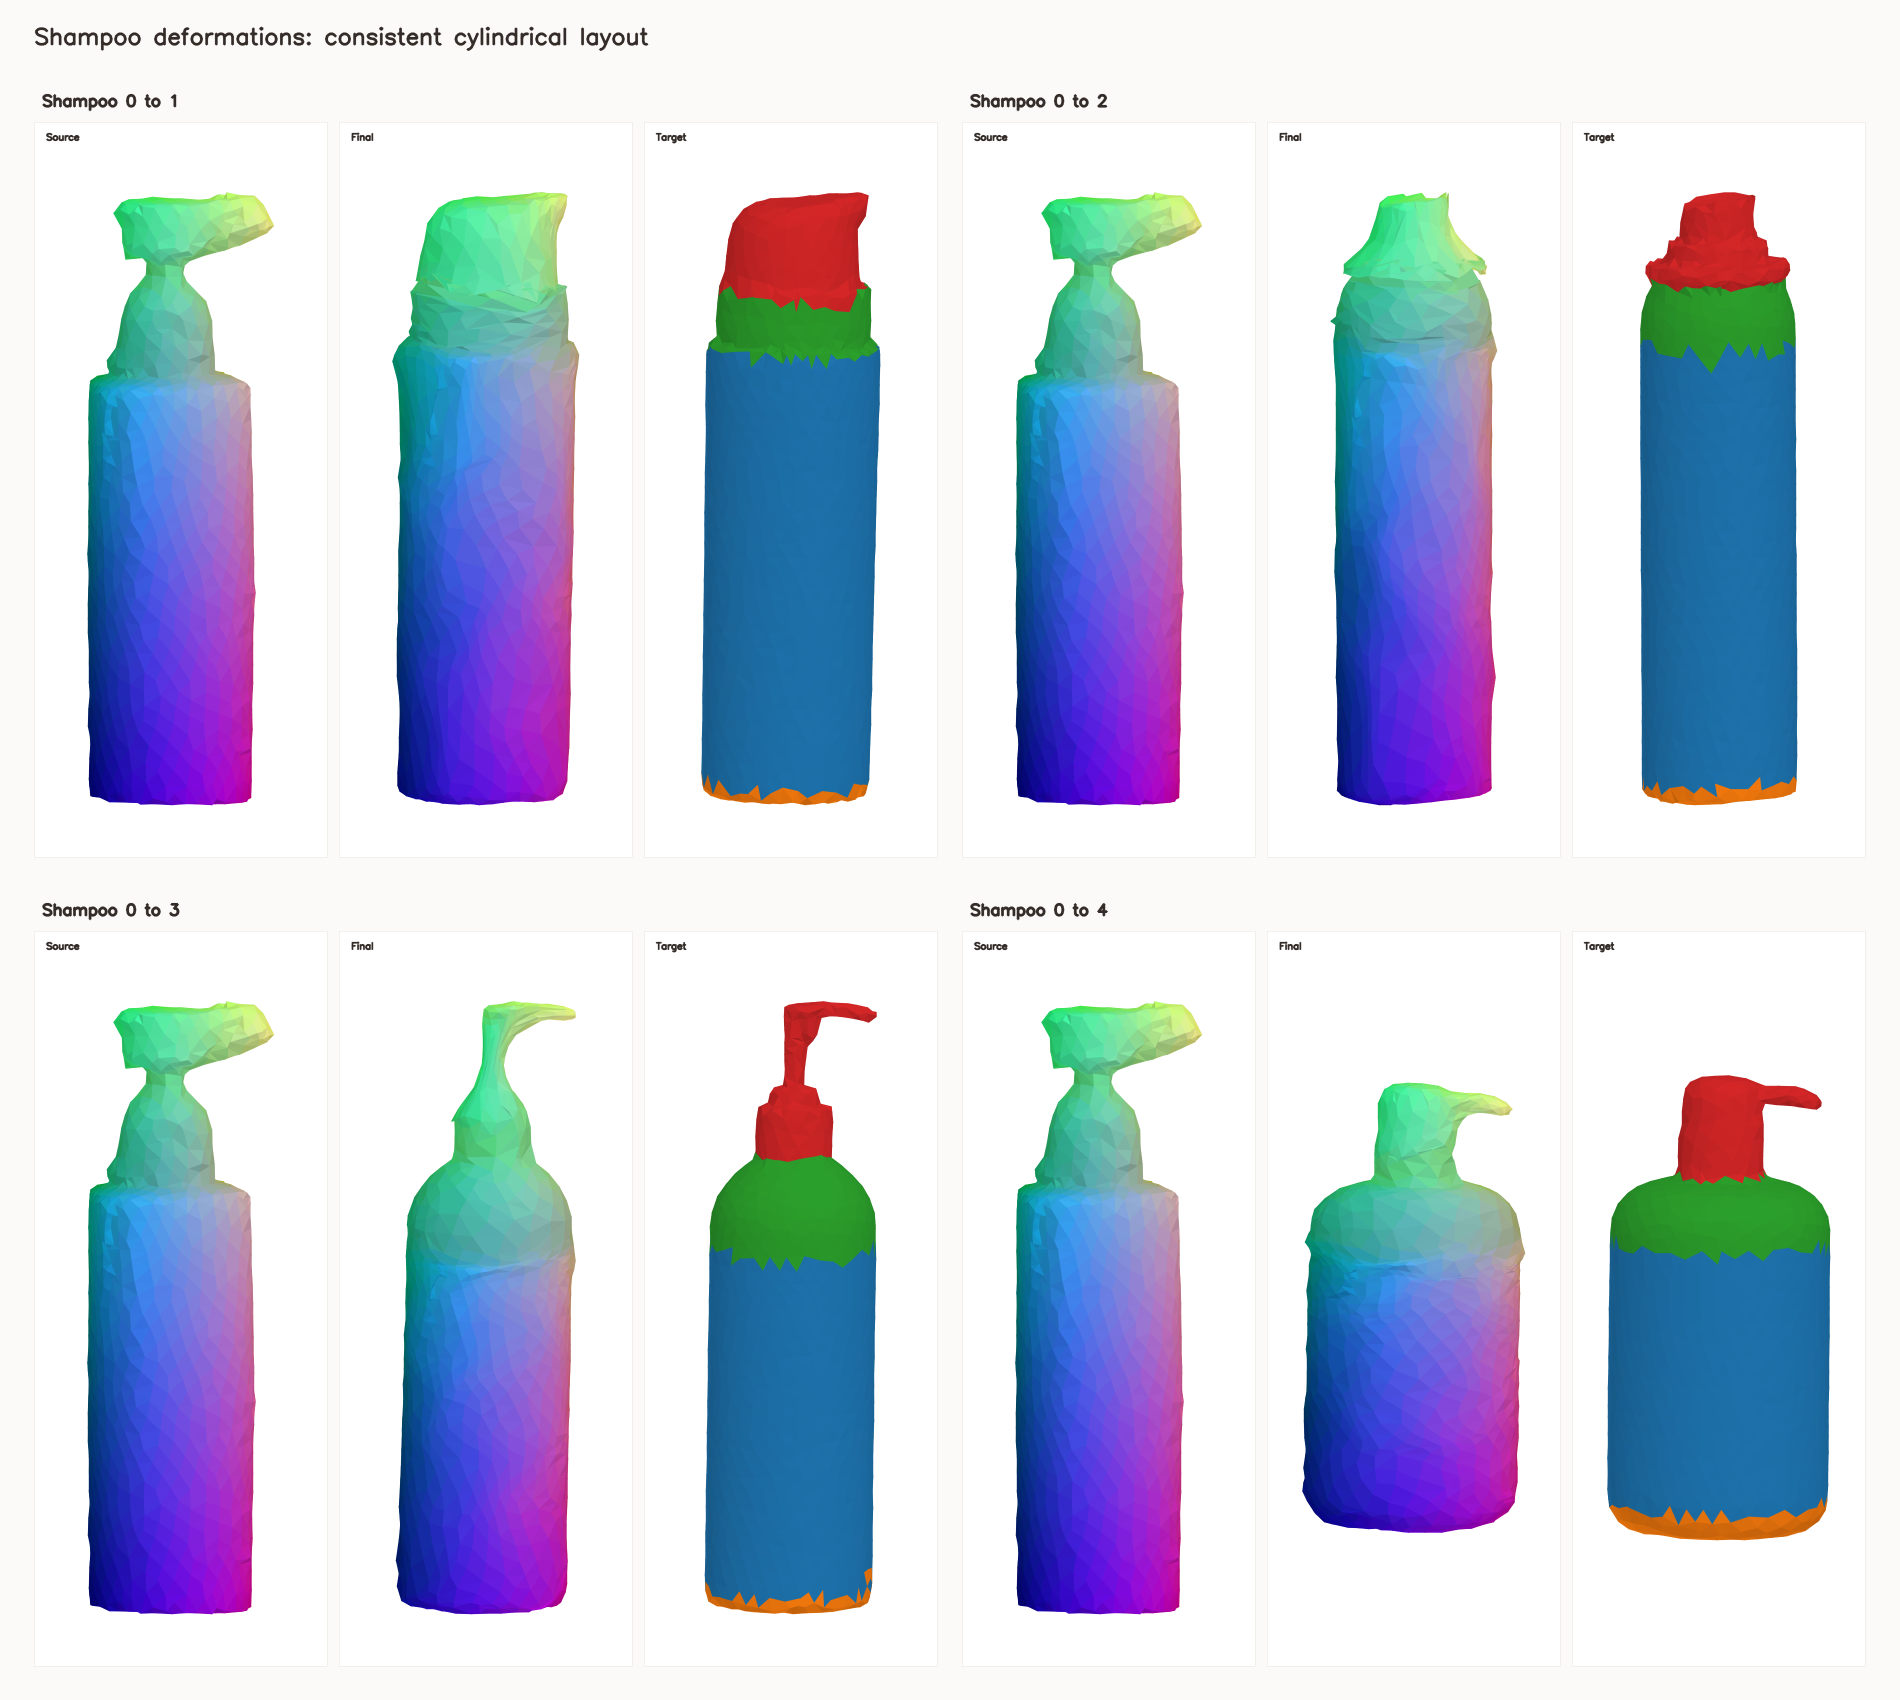
\includegraphics[width=0.90\textwidth]{figures/domain_shampoo_showcase.png}
\caption{Shampoo deformation showcase. The tall body/top structure is a clean PartField case.
Source and final panels use inherited source-position coloring; target panels use PartField bucket
coloring, so colors should be read as within-panel structure rather than direct cross-panel labels.}
\label{fig:domain-shampoo}
\end{figure}

\section{Local Chamfer Spike Failure Example}
\label{app:spike-failure}

Section~\ref{sec:loss-function} explains why an evenly-weighted, per-point local Chamfer term can
pull an unclaimed source point toward its own single nearest target point at full strength, with
nothing else to keep it near its neighbors. Figure~\ref{fig:spike-failure} shows a concrete instance
of this from an early exploration of the bulldog$\to$dachshund pair, using a PartField chamfer-only
objective ($\lambda_g=0$, no jump/edge-stretch regularization, and neither the asymmetric
source-to-target weighting nor the unmatched-point down-weight from Section~\ref{sec:loss-function}
enabled yet). The front leg collapses into a thin spike reaching well past the target's own leg
length, and the head develops a smaller spike above the ear. Introducing $\alpha < 1$ and the
unmatched-point down-weight $\gamma$ (Section~\ref{sec:loss-function}) reduced this failure mode
in later runs.

\begin{figure}[H]
\centering
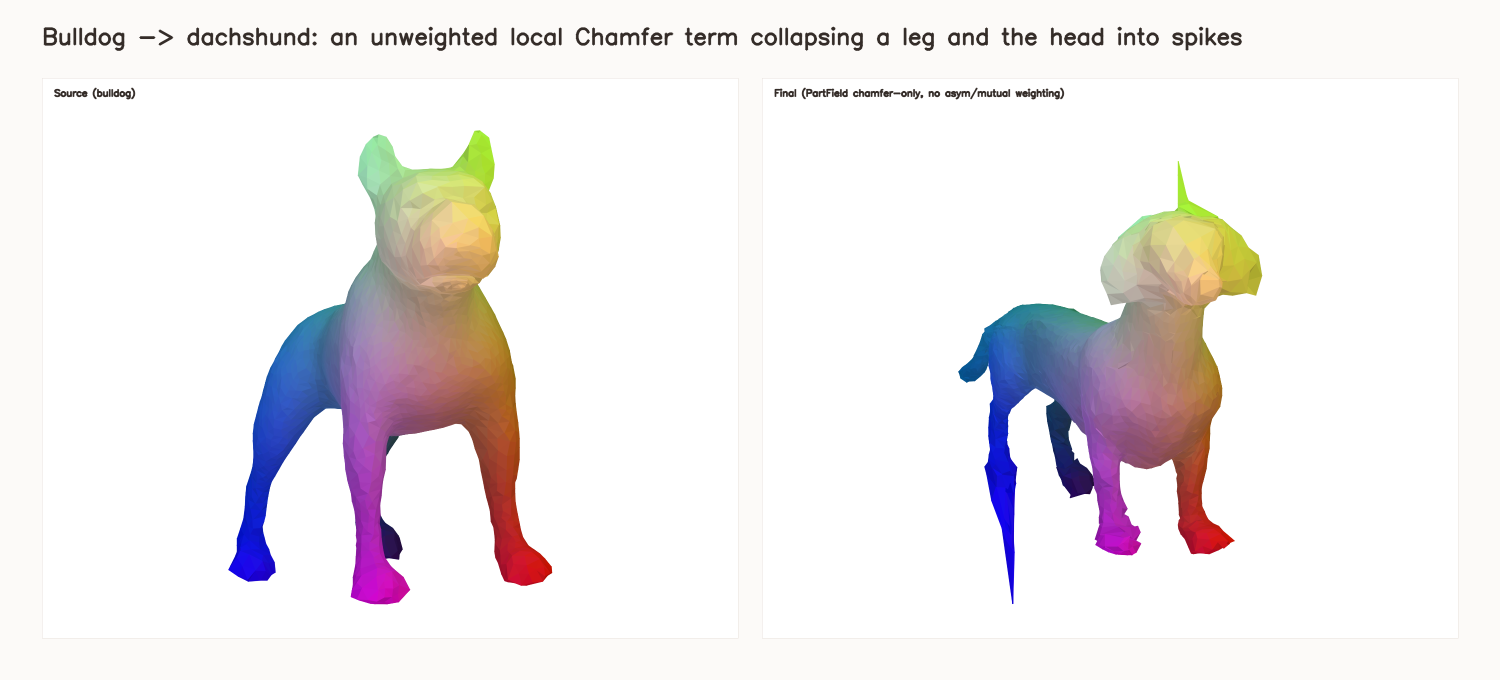
\includegraphics[width=0.95\textwidth]{figures/bulldog_dachshund_spike_failure.png}
\caption{Bulldog$\to$dachshund, PartField chamfer-only, before the asymmetric and unmatched-point
weighting described in Section~\ref{sec:loss-function} was introduced. The front leg and the
head each collapse into a thin spike rather than deforming smoothly. Coloring is inherited
source-position, consistent with the other deformation figures in this report.}
\label{fig:spike-failure}
\end{figure}

\section{PartField Granularity by Category}
\label{app:pf-granularity}

Section~\ref{sec:densematcher-fair} deliberately reports headline numbers under zero PF
selection (Table~\ref{tab:densematcher-full}'s ``PF range'' column) rather than a single
best-per-category granularity, precisely to avoid quietly picking a winner. That said, the
question of which single PartField granularity performs best per category is useful diagnostic
information in its own right. PF01 is the coarsest setting: it gives one bucket, so it provides
almost no part separation. Higher PF values create more buckets and can express more detailed
part structure, but the extra detail only helps when the shape really contains stable parts.
Table~\ref{tab:pf-best-per-category} reports the oracle best-single-PF value for every category,
computed the same way as the ``best PF per category'' rows in
Table~\ref{tab:densematcher-headline} (\AUC{}/\Err{} at that pair's single best-scoring
granularity, not averaged across the range).

\begingroup
\small
\setlength{\tabcolsep}{4pt}
\begin{longtable}{lcrr}
\caption{Best-scoring single PartField granularity per DenseCorr3D category (oracle, not the
zero-selection headline).}
\label{tab:pf-best-per-category}\\
\toprule
Category & Best PF & AUC & Err \\
\midrule
\endfirsthead
\toprule
Category & Best PF & AUC & Err \\
\midrule
\endhead
\bottomrule
\endfoot
animals & PF06 & 0.7443 & 7.432 \\
apple & PF05 & 0.8796 & 3.013 \\
backpack & PF04 & 0.8895 & 2.834 \\
banana & PF01 & 0.8607 & 3.485 \\
bell\_pepper & PF03 & 0.8056 & 5.079 \\
broccoli & PF02 & 0.6361 & 9.472 \\
carrot & PF04 & 0.7173 & 7.273 \\
cars & PF06 & 0.9476 & 1.332 \\
celery & PF06 & 0.9046 & 2.386 \\
chairs & PF08 & 0.9426 & 1.528 \\
cucumber & PF01 & 0.8287 & 4.299 \\
egg & PF03 & 0.9088 & 2.279 \\
eggplant & PF01 & 0.8159 & 4.601 \\
knife & PF02 & 0.9731 & 0.672 \\
mushroom & PF02 & 0.7986 & 5.322 \\
onion & PF02 & 0.8384 & 4.054 \\
peach & PF01 & 0.8984 & 2.540 \\
pear & PF02 & 0.8370 & 4.076 \\
potato & PF01 & 0.7829 & 5.428 \\
pumpkin & PF02 & 0.8785 & 3.037 \\
shampoo & PF03 & 0.9701 & 0.748 \\
tomato & PF02 & 0.9110 & 2.224 \\
zucchini & PF01 & 0.8797 & 3.008 \\
\end{longtable}
\endgroup

The pattern in Table~\ref{tab:pf-best-per-category} is fairly clean once the direction of PF is
kept straight. Categories with distinct, repeated, or articulated parts often prefer intermediate
to finer settings -- chairs (PF08: seat, back, legs, stretchers), cars (PF06), celery and animals
(PF06), backpack and carrot (PF04) -- because one or two buckets cannot represent their real
structure. Smooth or weakly differentiated produce often prefers very coarse settings, usually
PF01--PF02 (banana, cucumber, eggplant, mushroom, onion, peach, potato, pumpkin, zucchini), because
additional buckets split the surface into arbitrary rings or patches that do not correspond
reliably across instances. Broccoli is the exception that explains the limit: its best setting is
PF02, but even that cannot recover the irregular floret groups used by DenseCorr3D's annotation.

\section{Curriculum Ablation Diagnostic}
\label{app:curriculum-ablation}

The optimization is staged because the problem is non-convex. If fine part buckets are imposed too
early, the source can get trapped in a bad local minimum. If only coarse/global alignment is used
for too long, the optimizer may find a geometrically plausible but semantically wrong solution.
Because the ablation covers only 8 hard DenseCorr3D pairs, it is treated as a supporting diagnostic
rather than as part of the main benchmark claim.

\begin{table}[H]
\centering
\small
\begin{tabularx}{\textwidth}{>{\raggedright\arraybackslash}X>{\raggedright\arraybackslash}X>{\raggedright\arraybackslash}X}
\toprule
Stage & Purpose & Typical signal \\
\midrule
Coarse alignment & Move the source into the target's overall pose and scale. & Coarse surface and PartField guidance. \\
Part-aware fitting & Align corresponding local regions. & Local bucket Chamfer, bucket balancing, PF6--PF8. \\
Regularized refinement & Improve surface fit without destroying mesh quality. & Lower learning rate, regularization, edge and Jacobian penalties. \\
\bottomrule
\end{tabularx}
\caption{The staged deformation schedule used in the curriculum diagnostic.}
\label{tab:curriculum}
\end{table}

On 8 hard DenseCorr3D pairs, the three-stage curriculum improved both metrics over a single-stage
baseline on the majority of pairs (Table~\ref{tab:curriculum-ablation}): mean AUC rose from $0.804$
to $0.823$ ($6/8$ pairs improved) and mean Err fell from $6.05$ to $5.60$ ($6/8$ pairs improved).

\begin{table}[H]
\centering
\small
\begin{tabular}{lrrrr}
\toprule
Pair & Baseline Err & Curriculum Err & Baseline AUC & Curriculum AUC \\
\midrule
Elephant $\to$ Giraffe & 7.486 & 6.320 & 0.803 & 0.856 \\
Elephant $\to$ Moose & 5.856 & 5.172 & 0.799 & 0.830 \\
Giraffe $\to$ Bear & 0.778 & 0.805 & 0.969 & 0.968 \\
Moose $\to$ Cheetah & 7.138 & 6.740 & 0.740 & 0.763 \\
Moose $\to$ Giraffe & 10.465 & 9.623 & 0.727 & 0.748 \\
Moose $\to$ Panther & 8.385 & 7.692 & 0.694 & 0.718 \\
Panther $\to$ Giraffe & 2.150 & 2.078 & 0.916 & 0.926 \\
Panther $\to$ Moose & 6.144 & 6.360 & 0.781 & 0.778 \\
\midrule
\textbf{Mean} & \textbf{6.050} & \textbf{5.599} & \textbf{0.804} & \textbf{0.823} \\
\bottomrule
\end{tabular}
\caption{Three-stage curriculum vs.\ single-stage baseline, 8 hard DenseCorr3D pairs.}
\label{tab:curriculum-ablation}
\end{table}

\section{Evaluator Design Notes}
\label{app:evaluator-variants}

Because DenseCorr3D's official evaluator and its per-mesh geodesic distance matrices were never
published, Section~\ref{sec:densematcher-fair} implements its own graph-geodesic (Dijkstra) scorer
rather than reproducing DenseMatcher's published benchmark protocol; both methods are then re-scored
under that one evaluator, applied identically to both sides. A couple of design choices were tried
before settling on the version used throughout this report: scoring each directed pair with its own
matched direction (\texttt{surface\_map} vs.\ \texttt{surface\_map\_inv}) rather than averaging both
directions together, and using DenseMatcher's released correspondence map directly rather than an
ICP-refined or adjoint-refined variant of it. The production evaluator uses \texttt{surface\_map},
matched per pair by direction, exactly as described in Section~\ref{sec:densematcher-fair}.

\section{Supplementary Materials}
\label{app:supplementary}

An interactive video showcase accompanies this report: hover-to-play deformation clips for a range
of category pairs, alongside the headline comparison numbers against DenseMatcher from
Section~\ref{sec:densematcher-fair}. It is available at
\url{https://rona-latifaj-uni-freiburg.github.io/meshup-v2/}.

\begin{thebibliography}{99}

\bibitem{meshup}
Hyunwoo Kim, Itai Lang, Noam Aigerman, Thibault Groueix, Vladimir G. Kim,
and Rana Hanocka.
\newblock MeshUp: Multi-Target Mesh Deformation via Blended Score Distillation.
\newblock arXiv:2408.14899, 2024.
\newblock \url{https://arxiv.org/abs/2408.14899}.

\bibitem{dreamfusion}
Ben Poole, Ajay Jain, Jonathan T. Barron, and Ben Mildenhall.
\newblock DreamFusion: Text-to-3D using 2D Diffusion.
\newblock arXiv:2209.14988, 2022.
\newblock \url{https://arxiv.org/abs/2209.14988}.

\bibitem{dinov2}
Maxime Oquab, Timothee Darcet, Theo Moutakanni, Huy V. Vo, Marc Szafraniec,
Vasil Khalidov, Pierre Fernandez, Daniel Haziza, Francisco Massa, Alaaeldin
El-Nouby, and others.
\newblock DINOv2: Learning Robust Visual Features without Supervision.
\newblock arXiv:2304.07193, 2023.
\newblock \url{https://arxiv.org/abs/2304.07193}.

\bibitem{deepfloydif}
DeepFloyd and Stability AI.
\newblock DeepFloyd IF-I-XL-v1.0 Model Card.
\newblock Hugging Face, 2023.
\newblock \url{https://huggingface.co/DeepFloyd/IF-I-XL-v1.0}.

\bibitem{chamferl1}
Fangzhou Lin, Songlin Hou, Haotian Liu, Shang Gao, Kazunori D.~Yamada,
Haichong K.~Zhang, and Ziming Zhang.
\newblock Hyperbolic Chamfer Distance for Point Cloud Completion and Beyond.
\newblock \textit{arXiv preprint arXiv:2412.17951}, 2024.
\newblock \url{https://arxiv.org/abs/2412.17951}.

\bibitem{densematcher}
Junzhe Zhu, Yuanchen Ju, Junyi Zhang, Muhan Wang, Zhecheng Yuan, Kaizhe Hu,
and Huazhe Xu.
\newblock DenseMatcher: Learning 3D Semantic Correspondence for Category-Level
Manipulation from a Single Demo.
\newblock International Conference on Learning Representations, 2025.
\newblock \url{https://tea-lab.github.io/DenseMatcher/}.

\bibitem{partfield}
Minghua Liu, Mikaela Angelina Uy, Donglai Xiang, Hao Su, Sanja Fidler,
Nicholas Sharp, and Jun Gao.
\newblock PartField: Learning 3D Feature Fields for Part Segmentation and
Beyond.
\newblock International Conference on Computer Vision, 2025.
\newblock \url{https://arxiv.org/abs/2504.11451}.

\bibitem{sam3d}
SAM 3D Team: Xingyu Chen, Fu-Jen Chu, Pierre Gleize, Kevin J. Liang, Alexander Sax, Hao Tang,
Weiyao Wang, Michelle Guo, Thibaut Hardin, Xiang Li, Aohan Lin, Jiawei Liu, Ziqi Ma, Anushka
Sagar, Bowen Song, Xiaodong Wang, Jianing Yang, Bowen Zhang, Piotr Doll\'ar, Georgia Gkioxari,
Matt Feiszli, and Jitendra Malik (Meta AI).
\newblock SAM 3D: 3Dfy Anything in Images.
\newblock arXiv:2511.16624, 2025.
\newblock \url{https://arxiv.org/abs/2511.16624}.

\bibitem{psgn}
Haoqiang Fan, Hao Su, and Leonidas J. Guibas.
\newblock A Point Set Generation Network for 3D Object Reconstruction from a
Single Image.
\newblock Proceedings of the IEEE Conference on Computer Vision and Pattern
Recognition, 2017.
\newblock \url{https://openaccess.thecvf.com/content_cvpr_2017/html/Fan_A_Point_Set_CVPR_2017_paper.html}.

\bibitem{arap}
Olga Sorkine and Marc Alexa.
\newblock As-Rigid-As-Possible Surface Modeling.
\newblock Eurographics Symposium on Geometry Processing, 2007.
\newblock \url{https://doi.org/10.2312/SGP/SGP07/109-116}.

\bibitem{njf}
Noam Aigerman, Kunal Gupta, Vladimir G. Kim, Siddhartha Chaudhuri, Jun Saito,
and Thibault Groueix.
\newblock Neural Jacobian Fields: Learning Intrinsic Mappings of Arbitrary
Meshes.
\newblock ACM Transactions on Graphics, 41(4), 2022.
\newblock \url{https://arxiv.org/abs/2205.02904}.

\bibitem{tosca}
Alexander M. Bronstein, Michael M. Bronstein, and Ron Kimmel.
\newblock Numerical Geometry of Non-Rigid Shapes.
\newblock Springer, 2008.
\newblock \url{https://doi.org/10.1007/978-0-387-73301-2}.

\end{thebibliography}

\end{document}
